\documentclass[a4paper, twoside, 12pt]{book}
\usepackage[utf8]{inputenc}
\usepackage[T1]{fontenc}
\usepackage[french]{babel}

\usepackage{setspace}
\usepackage{longtable}
\usepackage{tabularx}
\usepackage{caption}
\usepackage{subcaption}
\usepackage{listings}
\usepackage{mdframed}
\usepackage[x11names]{xcolor}

\lstdefinestyle{mystyle}{
	backgroundcolor=\color{LavenderBlush1},   
	commentstyle=\color{Purple4},
	keywordstyle=\color{PaleVioletRed4},
	numberstyle=\tiny\color{Plum3},
	stringstyle=\color{Plum4},
	basicstyle=\ttfamily\footnotesize,
	breakatwhitespace=false,         
	breaklines=true,                 
	captionpos=b,                    
	keepspaces=true,                 
	numbers=left,                    
	numbersep=5pt,                  
	showspaces=false,                
	showstringspaces=false,
	showtabs=false,                  
	tabsize=2
}

\lstset{style=mystyle}



%Pour gérer caractères spéciaux °

%Pour les épigraphes
\usepackage{epigraph}
\setlength{\epigraphrule}{0pt}
\setlength{\epigraphwidth}{0.6\textwidth}
\renewcommand\textflush{flushepinormal}
\renewenvironment{flushepinormal}{}{\vspace*{-\baselineskip}}
\usepackage{booktabs} % Required for better table rules
% Title page details: 
%--------------------------
% HYPERREF (liens hypertextes et métadonnées)
%--------------------------
\usepackage{hyperref}
\hypersetup{%
	colorlinks=true,
	linkcolor=black,
	urlcolor=blue,
	citecolor=black
}

\title{Mémoire de Master 2}
\author{Mai Lan Lopez}

%--------------------------
% TOCBIBIND (ajouter la bibliographie dans la Table des matières)
%--------------------------
%\usepackage{tocbibind}
\usepackage[nottoc,notlot,notlof]{tocbibind}
%--------------------------
% Éléments de mise en page (marge de 2,5 cm, alinéa en début de paragraphe 1cm, interligne 1,5)
%--------------------------
\usepackage[a4paper, margin=2.5cm]{geometry}
\usepackage{setspace}
\onehalfspacing
\setlength{\parindent}{1cm}

\usepackage{fancyhdr}
\setlength{\headheight}{28pt}
\renewcommand{\chaptermark}[1]{\markboth{#1}{}}
\renewcommand{\sectionmark}[1]{\markright{#1}}
\pagestyle{fancy}
\fancyhf{}
\fancyhead[LE,RO]{\thepage}
\fancyhead[LO]{\nouppercase{\rightmark}}
\fancyhead[RE]{\nouppercase{\leftmark}}
\renewcommand{\headrulewidth}{0pt}

%--------------------------
% Modules pour gérer les listes
%--------------------------
\usepackage{enumerate}
\usepackage{enumitem}


%--------------------------
% BIBLIOGRAPHIE
%--------------------------
\usepackage[backend=biber, sorting=nyt, style=enc]{biblatex}
\usepackage[autostyle]{csquotes}
\addbibresource{biblio_zotero.bib}

\setcounter{secnumdepth}{5}
\setcounter{tocdepth}{2}

\usepackage[official]{eurosym}
\usepackage{afterpage}
\usepackage{booktabs,xltabular}
%--------------------------
% FIGURES
%--------------------------
\usepackage{graphicx}
\graphicspath{ {./images/} }
\usepackage{float}


% ============================================


\begin{document}
	
	\frontmatter
	\begin{titlepage}


\begin{center}

\bigskip

\begin{large}
UNIVERSITÉ PARIS, SCIENCES \& LETTRES
\end{large}

\begin{center}\rule{2cm}{0.02cm}\end{center}

\bigskip
\bigskip
\bigskip
\begin{Large}
\textbf{Mai Lan Lopez}\\
\end{Large}

\bigskip
\bigskip
\bigskip

\begin{Huge}
\textbf{DÉCRIRE SON TRAVAIL, ÉCRIRE SA CONDITION}\\
\end{Huge}

\bigskip
\bigskip
\begin{LARGE}
\textbf{Femmes et hommes domestiques dans la presse d'annonces (Paris, Lyon, Bordeaux, 1750-1815) }\\
\end{LARGE}

\bigskip
\bigskip
\bigskip
\vfill

\begin{large}
Mémoire de deuxième année du master\\
\og Humanités Numériques \fg{} \\
École nationale des chartes \\
\bigskip
2023
\end{large}

\end{center}
\end{titlepage}
	\section*{Résumé}
\addcontentsline{toc}{chapter}{Résumé}

Ce mémoire prend pour objet les petites annonces d'emploi domestique publiées entre le milieu du XVIIIè siècle et le début du XIXè siècle dans trois villes françaises, Paris, Lyon et Bordeaux. À travers l'exploitation numérique de ces sources, il vise à étudier à la fois l'économie générale des annonces, leur contenu, le profil socio-démographique des travailleuses et travailleurs qui les publient, et les différentes stratégies qui différencient ce support du marché traditionnel du travail. La mobilisation de méthodes de traitement automatique des langues est également l'occasion de s'intéresser aux formes de publicité de soi et de son travail qui composent l'annonce, et qui permettent d'identifier ce qui constitue la "bonne domesticité" à l'époque moderne.

\medskip

\textbf{Mots-clés: histoire moderne; humanités numériques ; études sur le genre ; traitement automatique de la langue ; apprentissage machine ; travail ; domesticité ; presse; petites annonces.}

\textbf{Informations bibliographiques:} Mai Lan Lopez, \textit{Décrire son travail, écrire sa condition: femmes et hommes domestiques dans la presse d'annonces (Paris, Lyon, Bordeaux, 1750-1815)}, mémoire de master 2 \og Humanités Numériques\fg{}, dir. Clyde Plumauzille, Marie Puren, Université Paris, Sciences \& Lettres, 2023.



\section*{Abstract}

This dissertation focuses on domestic job advertisements published between the mid-18th century and the early 19th century in three French cities: Paris, Lyon, and Bordeaux. Through the digital study of these sources, it aims to better understand the overall economy of the advertisements, their content, the socio-demographic profiles of the workers who published them, and the various strategies that distinguish this type of media from the traditional labor market. The use of Natural Language Processing methods also provides an opportunity to explore the forms of self-promotion and self-representation within these advertisements, allowing us to identify what constituted "good domestic service" in the modern era.

\medskip

\textbf{Keywords: modern history; digital humanities; gender studies; natural language processing; machine learning; work; domesticity; press; personal ads.}

\textbf{Bibliographic information:} Mai Lan Lopez, \textit{Describing labor, inscribing work: women and men domestic servants in personal ads (Paris, Lyon, Bordeaux, 1750-1815)}, M.A. thesis \og Digital Humanities\fg{}, dir. Clyde Plumauzille, Marie Puren, Université Paris, Sciences \& Lettres, 2023.


\clearpage
	
	% table des matières
	\addcontentsline{toc}{chapter}{Table des matières}
	\tableofcontents
	
	\mainmatter
	
	\part*{Introduction}
\addcontentsline{toc}{part}{Introduction}
\markboth{Introduction}{Introduction}


Il parait difficile de concevoir, de notre point de vue contemporain, la place qu'a pu occuper la domesticité dans le paysage urbain et social français avant le XXè siècle. Beaucoup d'indices, néanmoins, mettent en exergue le rôle économique et culturel considérable des domestiques, à commencer par leur poids démographique: l'historiographie moderne considère qu'ils et elles représentent entre 5 et 15\% de la population selon les villes, des chiffres qui fluctuent beaucoup selon les conjonctures. À Paris, au XVIIIè siècle, Jacqueline Sabattier estime qu'ils et elles représentent environ 50 000 personnes, soit 10\% de la population, et que leur proportion tend à augmenter pendant le siècle. Une famille parisienne sur quatre emploierait alors au moins un ou une domestique\footcites[p.28]{mazaServantsMastersEighteenthcentury1983}.

Ombres et témoins de leurs maîtres, omniprésents au théâtre, dans la littérature et dans les traités de police mais invisibles ou presque dans les sources de la pratique et les archives du for privé, les domestiques ont pendant longtemps moins intéressé la discipline historique que d'autres catégories de population, mieux représentées dans les sources (compagnons, apprentis, ouvrières ...). Du fait de leur association avec la noblesse puis la bourgeoisie, les domestiques ont longtemps été tenus à l'écart de l'étude des populations laborieuses et dominées, dont le cœur a toujours été la condition ouvrière. 

Depuis la seconde moitié du XXè siècle, néanmoins, l'histoire démographique, puis l'histoire du travail, ont semblé ouvrir le grand chantier de l'histoire de la condition ancillaire. Portée notamment par des projets de recherche à l'échelle européenne\footcites{pasleauProceedingsServantProject2001}, celle-ci a fait l'objet dès la fin des années 1980 de synthèses qui font encore date aujourd'hui, notamment grâce aux statistiques qu'elles fournissent sur ce groupe peu connu\footcites{sabattierFigaroSonMaitre1984,guttonDomestiquesServiteursDans1981,fairchildsDomesticEnemiesServants1984, mazaServantsMastersEighteenthcentury1983}. À partir des sources de l'histoire sociale (notamment les insinuations testamentaires, les contrats de mariage et les déclarations de grossesse), la discipline a peu à peu contribué à la formation d'acquis historiographiques forts sur la domesticité, une population pourtant caractérisée par sa diversité interne. 

L'histoire du genre, enfin, s'est également emparée du sujet à partir des années 2000, en le retravaillant à l'aune de la féminisation croissante du secteur à partir de la fin du XVIIIè siècle, de l'association culturelle et matérielle des femmes au foyer et aux activités domestiques, puis avec l'outil théorique du \textit{care}. 

C'est nourrie de ces différentes approches et traditions historiographiques que je cherche dans ce mémoire à étudier la domesticité du XVIIIè siècle à partir d'une source peu mobilisée jusque-là par les historiennes et historiens du travail: la presse d'annonces. 


\section{Histoire de la presse d'annonces en France}

\subsection{La naissance des journaux d'annonces}

Le premier journal d'annonces français naît à Paris au XVIIè siècle\footcite{martinTroisSieclesPublicite1992}; il est à l'époque une émanation du Bureau d'adresses ouvert en 1630 par le médecin et proche du cardinal Richelieu Théophraste Renaudot, "pour le règlement général des pauvres". Moins de dix ans plus tard, une ordonnance royale oblige les travailleurs sans emplois à s'y présenter; le Bureau est lié, dès sa naissance, "à la grande entreprise de mise en ordre de la société française par la monarchie absolue naissante". Théophraste Renaudot obtient à la même époque le privilège de la \textit{Gazette}, qui deviendra le principal organe de presse du royaume et un outil de propagande essentiel pour les acteurs de la monarchie, Richelieu en tête.

C'est également peu après l'ouverture du Bureau que les \textit{Feuilles d'adresses} commencent à être diffusées, à l'époque tous les dix jours. Elles répertorient les demandes et les offres déposées au Bureau, tout en faisant la publicité du dispositif, mais n'ont pas encore vocation à devenir une publication à part entière. En 1641, face au succès du Bureau de l'île de la Cité, une deuxième adresse ouvre ses portes sous les galeries du Louvre. Après la mort du cardinal Richelieu en 1646, puis de Louis XIII et enfin de Renaudot lui-même en 1653, la diffusion des\textit{ Feuilles} (ou \textit{Liste}, comme elles sont parfois appelées) devient beaucoup plus disparate. Le Bureau d'adresses est confié par le fils Renaudot à des concessionnaires, qui assurent sa subsistance mais ne lui permettent plus de connaître le succès qu'il avait rencontré à ses débuts.

\subsection{La renaissance et l'établissement des\textit{ Affiches} au XVIIIè siècle}

Au milieu du XVIIIè siècle, le format de la petite annonce est ressuscité par plusieurs initiatives individuelles, pour la première fois stables et durables, inspirées du succès du format à l'étranger, notamment en Allemagne. Les annonces font leur apparition dans les titres généralistes, mais également dans des publications spécialisées et dédiées aux petites annonces. La famille Renaudot cède ainsi en 1749 les privilèges de la \textit{Gazette} et du Bureau d'adresses; les deux entrepreneurs qui les récupèrent lancent successivement en 1751 les \textit{Affiches de Paris} puis en 1752 les \textit{Affiches de province}. Le modèle économique des deux publications repose sur l'abonnement: relativement cher, réservé à un lectorat plutôt fortuné (qu'Ulrike Krampl désigne comme "consommateurs éclairés"), il garantit la gratuité du dépôt des annonces par, entre autres, les domestiques en recherche d'un emploi. Face au succès de l'édition parisienne, des versions régionales paraissent, dont celles qui m'intéressent ici: les \textit{Affiches de Lyon} au début des années 1750, puis les \textit{Affiches de Bordeaux} en 1758.
À l'origine bi-hebdomadaires, au format de huit pages in-octavo, les \textit{Affiches de Paris} deviennent quotidiennes à la fin des années 1770. Au total, vers 1780, elles publient 3 000 à 5 000 annonces par mois, pour des tirages à 3000 exemplaires, qui doublent encore dans les dix années suivantes. En 1788, face au rythme des demandes, que le journal ne parvient à soutenir malgré la publication régulière de suppléments de huit ou seize pages, la publication d'une annonce devient payante, au prix d'une livre quatre sols\footcites{kramplPresseAnnoncesParisienne2020}. 

\subsection{Annonces et recherche d'emploi, une apparition plus tardive}


Le contenu des \textit{Affiches}, dès leurs débuts, se caractérise par une grande diversité, et est organisé par rubriques: annonces commerciales évidemment, immobilières (vente ou location) ou mobilières (meubles, chevaux, voitures), publicités (notamment relatives aux parutions des libraires), informations (mariages, enterrements) ou recherche d'informations (objets perdus). Certains titres publient même les programmes des salles de théâtre, les dernières décisions de justice ou le cours des monnaies. La seule catégorie qu'on n'y trouve pas (encore) est celle de la recherche matrimoniale, qui n'investira ce support que plus tard, et plutôt dans des publications spécialisées. 

Les annonces d'emploi, quant à elles, apparaissent à Paris en 1760. Elles sont d'abord majoritairement des offres d'emploi, probablement du fait du caractère encore relativement intimiste des \textit{Affiches} en dehors de son "lectorat éclairé". Au cours des années 1770, les demandes deviennent progressivement majoritaires. Au total, entre 1760 et 1788, 19 000 annonces d'emploi sont publiées, dont trois quarts sont des demandes\footcites{kramplPresseAnnoncesParisienne2020}. 
Pour ce qui est des \textit{Affiches provinciales}, ces chiffres et ces informations relatives à la place des annonces d'emploi dans l'économie du journal n'ont, à ma connaissance, jamais été relevés.


\section{Presse, travail et humanités numériques}

\subsection{Presse, presse d'annonces et travail dans l'historiographie}

Face à l'histoire riche de la presse d'annonces en France depuis le XVIIè siècle, quel intérêt historiographique pour cet objet, quel usage par la discipline historique de ces sources?

Les journaux d'annonces ont d'abord été intégrés à l'histoire plus générale de la presse, notamment à partir de sa massification au XIXè siècle. L'ouvrage de référence sur la question\footcites{feyelAnnonceNouvellePresse2000}, issu de la thèse de Gilles Feyel, présente la particularité de se concentrer sur deux titres: un journal généraliste, la \textit{Gazette}, et les \textit{Affiches}, analysées au prime de la "presse d'information". L'ouvrage de synthèse de Marc Martin\footcites{martinTroisSieclesPublicite1992}, quant à lui, leur consacre un chapitre, mais les inclut dans une histoire plus générale de la publicité.

En tant qu'objet historique à part entière, et en tant que sources permettant de sonder les pratiques et les discours du monde social, la "quatrième page" n'a donc que très récemment intéressé les historiennes et les historiens. Quand elle est mobilisée, c'est principalement au prisme de trois objets, historiques ou sociologiques:  "le marché matrimonial, le marché du travail, et dans une moindre mesure le marché immobilier\footcites{frydmanEcrireHistoirePetites2020}". SI elle sert souvent de source d'appoint ou de contrepoint documentaire, elle reste rarement étudiée pour elle-même.

Dans le cadre de l'étude de la recherche de travail, les petites annonces ont pourtant montré leur potentiel heuristique, notamment lorsqu'il s'agit de s'intéresser aux catégories subalternes ou éloignées du marché traditionnel de l'emploi\footcites{bresseyLookingWorkBlack2010}{alvesRosieRiveterJob2012}. Pour le XVIIIè siècle français, c'est principalement l'historienne Ulrike Krampl qui s'est intéressée à un marché très largement occupé par la domesticité urbaine, et où se trouve surreprésentée une certaine condition ancillaire, plus qualifiée et masculine que la moyenne\footcites{kramplPresseAnnoncesParisienne2020,kramplTravaillerAvecLangues2019}. 

\subsection{Le renouveau des Humanités numériques: de la numérisation des sources...}

Face à cet intérêt limité de la recherche pour les journaux d'annonces, les projets de numérisation et de mise à disposition massive de la presse française et européenne depuis les années 2010 (\textit{Europeana newspaper}, NewsEye, Médias 19, RétroNews) représentent autant d'opportunités de se ressaisir de cet objet, voire peut-être même d'en faire émerger de nouveaux, propices à l'investigation numérique\footcites{pinsonLirePresseXIXe2017}. 


\subsection{...à leur exploitation numérique}

Plus que la simple numérisation, c'est en effet l'interrogation de la presse et de la presse d'annonces avec les outils des humanités numériques qui m'intéressent ici. Ces outils se sont en effet déjà révélés prometteurs pour penser le genre de la presse et du travail: la journée d'études du projet NewsEye qui s'est tenue en 2021 à la Bibliothèque nationale de France portait ainsi sur les femmes dans la presse ancienne numérisée. Les premières publications du projet ANR Numapress, ont également pris pour objet les rapports de sexe à l'aune de la "civilisation du journal", en s'intéressant aux titres de presse en eux-mêmes mais également aux "femmes de presse". Les projets "Gender and Work\footnote{Site du projet: \url{https://www.gaw.hist.uu.se/}}" et "Freedom on the Move\footnote{Site du projet: \url{https://freedomonthemove.org/}}", à partir d'objets radicalement différents, ont eux aussi permis de prendre conscience des capacités des méthodes numériques pour faire émerger des individus, des paroles et des pratiques jusque-là marginales\footcites{laiteEmmetInchSmall2020} dans la "grande histoire". 


\section{Corpus et méthodologie}


En prenant en compte ces différentes pistes amenées par l'histoire du travail, l'histoire du genre, l'histoire de la presse et les humanités numériques, ce projet vise à faire l'histoire des domestiques dans la presse d'annonces de trois villes françaises entre le milieu du XVIIIè et le début du XIXè siècle.  

À partir des cas de Paris, Lyon et Bordeaux, trois espaces urbains mais à la composition socio-économique différente sous l'Ancien Régime, il s'agit ici d'interroger à la fois le phénomène de massification de l'annonce d'emploi au XVIIIè siècle à l'aune d'outils quantitatifs, la composition socio-démographique, et notamment genrée, de la population qui publie des annonces et le contenu-même des annonces grâce aux méthodes du traitement computationnel des langues. Il s'agira ensuite de comparer les résultats obtenus avec les acquis de l'historiographie classique de la domesticité, mais également avec ceux, plus récents, de l'histoire du travail dans les annonces. 

Le corpus, dont le processus de constitution sera détaillé dans le chapitre 1 (et dont la composition précise peut être retrouvée en annexe), est donc formé de trois titres de presse d'annonces, les \textit{Affiches de Paris}, les \textit{Affiches de Lyon} et les \textit{Affiches de Bordeaux}, dont plusieurs milliers de numéros ont pu être récupérés.

La méthodologie a principalement reposé sur l'élaboration de scripts Python à l'aide de librairies de science des données (pandas, numpy) et de traitement automatique des langues (spacy, gensim, BERTopic, Top2Vec). Pour certaines parties du corpus, j'ai entraîné un modèle d'apprentissage, d'extraction et de catégorisation d'entités, qui m'a permis d'automatiser en partie le processus de segmentation des annonces.

Une première partie du mémoire s'intéressera au processus d'élaboration du corpus, qui s'est découpé en plusieurs étapes: récupération des titres numérisés sur des bibliothèques en ligne, océrisation des numéros, segmentation des textes obtenus, sélection des seules annonces d'emploi, puis correction et pré-traitement de celles-ci. Ensuite, une première exploration des annonces s'intéressera aux données socio-démographiques qui peuvent être extraites du corpus, et à ce que ces statistiques nous disent de la représentativité ou des disparités entre population générale et population des annonces. Puis c'est le corps-même de l'annonce qui fera l'objet d'un examen: les compétences mises en avant, les qualités invoquées et les emplois recherchés par les domestiques sont autant d'indices de l'état du marché du travail domestique. Les adresses et intermédiaires mobilisés à la fin des annonces seront ensuite investigués dans la quatrième partie, en vue de replacer le support du journal parmi l'ensemble des réseaux de cooptation et d'intermédiation qui co-existent au XVIIIè siècle. Enfin, la cinquième et ultime partie se penchera sur les apports des méthodes de \textit{topic modeling} pour la compréhension globale du corpus.

	\part{Constituer un corpus de petites annonces}



\chapter{Récupérer les journaux d'annonces}

Une fois choisis les journaux d’annonces qui constitueront le corpus\footnote{La constitution détaillée du corpus, comprenant notamment le nombre de numéros récupérés par année, est disponible en annexe.}, j’ai employé des méthodes de \textit{web scraping} pour récupérer leurs versions numérisées sur les bibliothèques numériques de chaque ville : Gallica pour les \textit{Affiches} de Paris, Numelyo pour Lyon, Séléné pour Bordeaux. 

\section{Les \textit{Affiches} de Paris}

Le journal d’annonces de Paris au XVIIIè siècle,\textit{ Annonces, affiches et avis divers} (parfois\textit{ Affiches, annonces et avis divers}), est disponible sur Gallica de 1752 à 1814. Pour récupérer les numéros disponibles, j’ai choisi d’utiliser le \textit{wrapper} Pyllica, qui est spécialement conçu pour la récupération de périodiques via l’API IIIF. En effet, là où d’autres librairies Python (PyGallica, Gallipy) fonctionnent avec l’identifiant d’un document unique, Pyllica permet d’extraire un ensemble de numéros de journaux en précisant le nombre de documents à extraire et la fréquence d’extraction. Pyllica fonctionne sur la base de deux scripts : un premier qui définit une fonction d’extraction jpgpress ; un second qui appelle la fonction, dont l’utilisateur doit alors préciser les paramètres : url gallica du périodique à extraire, titre du fichier à créer, date de début d’extraction, nombre de numéros à extraire, fréquence d’extraction (tous les x jours), nombre de pages par numéro. Par exemple, l'exportation de trente et un numéros quotidiens, de la première à la trentième page, à partir du 1er janvier 1800, se fera avec les paramètres suivants:

\bigskip

\fbox{%
	\begin{minipage}{0.8\textwidth}
		from pyllicalabsjpgpress import *
		
		jpgpress(url="https://gallica.bnf.fr/ark:/12148/cb32683112b/date",
		title="journal", 
		year=1800, month=1, day=1, 
		item=31, rate=1, 
		firstpage=1, lastpage=30)
	\end{minipage}
}




\bigskip

Avant de parvenir à récupérer les images, il m’a fallu amender le premier script, qui répondait aux anciennes normes de Gallica (début d’adresses web en http au lieu de https). En sortie, on obtient ainsi un ensemble d’images jpg, intitulées au format « titre\_année\_mois\_jour\_page ».

Le nombre de numéros disponibles par an varie : pour la majorité des années, surtout de 1752 à 1780, l’intégralité des parutions hebdomadaires (environ 52 numéros par an) ou bihebdomadaires (environ 100 numéros par an) est numérisée. Dans ce cas-là, le choix a été fait de récupérer un numéro par semaine, afin de limiter le temps de récupération, et par commodité par rapport à la méthode de récupération choisie. En effet, Pyllica permet de récupérer des numéros de périodique tous les x jours de publication : on peut choisir de récupérer tous les numéros d’un quotidien en choisissant un pas d’un jour, ou tous les numéros d’un hebdomadaire en choisissant un pas de sept jours, mais les parutions bi-hebdomadaires nécessitent de faire tourner le script deux fois. 

Parfois, l’intégralité ou presque des journaux est disponible, mais les numéros ont été numérisés en une, deux, cinq ou dix fois, sans distinction des numéros par date de parution ; le document numérisé est par exemple mis à la date du 1er janvier de l’année, et fait alors plusieurs centaines de pages d’un coup. C’est le cas des années 1781, 1782, 1789, 1790, 1793, 1794. Dans ce cas, j’ai choisi de ne pas récupérer les journaux, jugeant que le travail de séparation et de datation de chaque numéro serait trop important.

Enfin, pour les numéros du début du XIXè siècle, j’ai fait le choix de récupérer l’ensemble des numéros disponibles, et plus seulement 52 par an, afin de pallier à l’absence de numérisation de nombreuses années de cette période (seules 1804, 1807, 1808 et 1814 sont disponibles) et de rééquilibrer le corpus par rapport aux années 1750-1780. Malheureusement, des restrictions de serveur liées à une refonte de l’API de Gallica m’ont empêchée de récupérer les numéros de 1808 et 1814. 



\section{Les \textit{Affiches} de Lyon}

Les \textit{Affiches} de Lyon, quant à elles, ont été numérisées de 1750 à 1804, avec d’importantes lacunes, notamment entre 1772 et 1795. Elles ont été récupérées à partir de la bibliothèque numérique de la ville de Lyon, Numelyo. Contrairement à Paris et Bordeaux, les numéros étaient cette fois rassemblés par année ou par ensemble de deux ou trois années. Après les avoir téléchargés, il a donc fallu disséquer les documents et leur assigner une date de parution précise. La tâche a été simplifiée par le fait que les numéros font en grande majorité quatre pages, publiés à intervalles réguliers, ce qui a permis d’automatiser une partie du processus ; mais certaines exceptions (suppléments ou compléments publiés en dehors des jours habituels, jours de fêtes qui empêchent la publication…) ont nécessité une vérification à la main. 


\section{Les \textit{Affiches} de Bordeaux}

La récupération des \textit{Annonces, affiches et avis divers pour la ville de Bordeaux} a été la moins automatique, et la moins complète. En effet, la bibliothèque numérique de la ville (Séléné) ne dispose pas d’API, et il n’a pas non plus été possible de récupérer les images disponibles à l’aide d’un script Python et de la librairie \textit{request}, les images étant mises en ligne à l’aide d’un lecteur pdf intégré.
Pour les vingt-trois années disponibles en ligne, de 1758 à 1784, j’ai donc fait le choix de télécharger à la main un numéro par mois. Les \textit{Affiches} de Bordeaux seront donc employées surtout à des fins de comparaison avec Paris et Lyon ; leur mode de récupération les rendent évidemment très minoritaires dans le corpus.

\bigskip

Une fois extraites les images disponibles pour les trois villes, j’ai cherché à unifier et à préparer au mieux mon corpus pour l’océrisation. J’ai tout d’abord utilisé un script Python pour uniformiser les noms de fichiers au format « Annonces\_ville\_année\_mois\_jour\_page ». Pour Bordeaux, j’ai converti les images de pdf à jpg avant de rassembler les images dans des dossiers par ville, puis par année, puis par mois.



\chapter{Océriser les journaux d'annonces}

\section{Un premier essai infructueux avec Tesseract}

Face à la qualité médiocre de l’OCR interne de Gallica, et surtout face à l’absence d’océrisation disponible pour Lyon et Bordeaux, j’ai tout d’abord envisagé d’utiliser le logiciel de reconnaissances optiques de caractères Tesseract. Néanmoins, après l’avoir testé en ligne de commande sur quelques numéros, j’ai pu observer que l’algorithme de Tesseract produisait beaucoup d’erreurs, notamment en tentant d’océriser tout ce qui n’était pas du texte au sein du journal (enjolivures en haut et bas de page, ornements autour des titres, caractères spéciaux à visée décorative, …). De plus, l’algorithme, peu adapté aux documents historiques, performait assez mal lorsque la numérisation était imparfaite, que les caractères étaient légèrement effacés par le temps, ou dès qu’il y avait des tâches sur les pages. Pour la petite dizaine de pages que j’ai testée avec Tesseract, j’ai ainsi obtenu des taux d’erreurs caractères (\textit{Character Error Rate}, ou CER) compris entre 5 et 10 \%, et des taux d’erreurs mots (\textit{Word Error Rate}, ou WER) compris entre 10 et 20 \%. Ces scores ne sont pas complètement mauvais mais ne représentent pas non plus une performance d’océrisation assez bonne pour les usages que je souhaitais faire des petites annonces.


\section{Le choix de Pero-OCR}

Après avoir envisagé un temps d’entraîner Tesseract sur mon corpus (une perspective abandonnée par manque de temps), j’ai ensuite pu tester, grâce à une suggestion de Marie Puren, l’algorithme de Pero-OCR. Pero est un moteur OCR conçu dans le cadre d’un projet entre l’université de technologie de Brno et la bibliothèque morave (République tchèque) visant à développer des outils pour l’exploitation et l’océrisation de documents historiques imprimés. Il a tout particulièrement été entraîné sur des journaux et des documents tchèques de basse qualité des XVIIIè et XIXè siècles\footnote{Ces informations sont disponibles sur le site du projet PERO: https://pero.fit.vutbr.cz/, ainsi que sur le Github du projet: https://github.com/DCGM/pero-ocr}, mais produit de bonnes performances pour la plupart des langues en alphabet latin, y compris le français\footcites{birkholzEvaluatingMultilingualCapabilities2021}. Par ailleurs, il dispose d’une interface en ligne, qui m’a permis de tester l’algorithme avant de l’implémenter grâce à la librairie Python associée. J’ai constaté à la suite de ces premiers tests que l’océrisation avec Pero était très bonne ; en calculant les scores d’erreurs mots et caractère, j’ai observé que ceux-ci se situaient en moyenne aux alentours de 1 \%, souvent pour des erreurs assez négligeables, d’accents ou de signes de ponctuation. Ayant jugé que ces résultats étaient déjà suffisamment bons sans avoir besoin de corriger et de relancer un entraînement de l'algorithme, je n’ai pas utilisé cette fonctionnalité de l’interface en ligne. Je suis donc passée directement à l’élaboration d’un script Python pour l’océrisation des journaux d’annonces.


Ce script prend en entrée les fichiers jpg ou tif des journaux numérisés, et me fournit en sortie des fichiers XML comprenant à la fois les informations de segmentation des pages et d’océrisation du texte. Le processus d’océrisation via la librairie Python repose sur la fonction « process\_page » , et sur un fichier de configuration (dans mon cas, le fichier « config\_file.ini » fourni intialement avec la librairie ; en cas d’entraînement de Pero sur l’interface web, il est possible de générer d’autres fichiers .ini adaptés). Par ailleurs, le script utilise la librairie de traitement d’image OpenCV pour lire les documents d’entrée page par page. Pour obtenir un fichier XML en sortie, j’ai utilisé la fonction « to\_pagexml ». 

\bigskip

\begin{lstlisting}[language=Python,caption=Code Pero-OCR]

import os
import configparser
import cv2
from pero_ocr.document_ocr.layout import PageLayout
from pero_ocr.document_ocr.page_parser import PageParser

path="./Annonces"

os.chdir(path)
for subdir,dirs,files in os.walk(path, topdown=True):
for file in files:
if file.endswith(".jpg") or file.endswith(".tif"):
path_file=os.path.join(path, subdir)
os.chdir(path_file)

# configuration
config_path = "./pero-ocr-modele/config.ini"
config = configparser.ConfigParser()
config.read(config_path)
page_parser = PageParser(config, config_path=os.path.dirname(config_path))
input_image_path = os.path.join(path_file, file)

# lecture de l'image
image = cv2.imread(input_image_path, 1)
page_layout = PageLayout(id=input_image_path,page_size=(image.shape[0], image.shape[1]))

# OCR
page_layout = page_parser.process_page(image, page_layout)

# nouveau dossier pour stocker l'OCR
path_resultats="./OCR_Annonces"
os.chdir(path_resultats)
nom_dossier_resultats="OCR_"+os.path.splitext(os.path.basename(path_file))[0]
if not os.path.exists(nom_dossier_resultats):
os.mkdir(nom_dossier_resultats)
new_path_resultats=os.path.join(path_resultats, nom_dossier_resultats)
os.chdir(new_path_resultats)
nom_fichier='OCR_'+os.path.splitext(os.path.basename(file))[0]+'.xml'

# enregistrement du fichier XML
page_layout.to_pagexml(nom_fichier)
			
\end{lstlisting}

\bigskip
		

\begin{table}[!htbp]
	\centering
	\begin{tabularx}{\textwidth}{|X|X|X|}
		\toprule
		\textbf{\textit{Gold standard} : texte transcrit à la main}        & \textbf{Tesseract (WER=13.1\%; CER=6.6\%)}                              & \textbf{Pero-OCR (WER=1.7\%; CER=0.6\%})  \\
		\midrule
		(935) donner des nouvelles à M. Simon, marché St.-Jean, no 3, recevra la récompense promise. DEMANDES. On desireroit trouver à louer aux environs de Paris, soit à Passy, Auteuil, Chaillot, Meudon, etc., une petite MAISON sise en bon air, ou un Appartement complet, pour trois mois de la belle saison. S'ad. par écrit ou verbalement, au portier du bureau de ce Journal. Demander la lettre D. On desireroit louer ou acheter une petite MAISON de campa- gne à Fontenay-aux-Roses, Meudon, ou à pareille distance de Paris, dans le prix de 10 à 15,000 fr. On voudroit qu'il y eût petit bâtiment et grand jardin. S'ad. par écrit à M. Levol, chef de bureau à l'hôtel de la Monnoie. Une personne âgée de 26 ans, sachant faire une cuisine bour- geoise, coudre, blanchir et parfaitement soigner les enfans, desireroit trouver une PLACE chez une personne de l'un ou l'autre sexe, soit pour Paris ou la campagne. S'adr. rue Coquillère, no. 52, au second, la porte à gauche. Une personne âgée de 32 ans, sachant faire une cuisine bourgeoise, coudre, blanchir et faire tout ce qui concerne le ménage, desireroit se PLACER dans une maison honnête (...). & . 7. “ | oo ( 935 ) donnerà des nouvelles à M. Simon , marche St.-Jean, no. 3, recevra la récompense promise, oo DEMANDES. Où desireroit trouver à louer aux environs de Paris , soit à Passÿ, Aateuil, Chaillot, Meudon , etc., une petite Maxon êise eu bon air, où uu Appartement complet, pour treis mois de la belle saison. S’ad. par écrit ou verbalement , au portier du bureau de ce Journal. Demander la lettre D. | Oa desireroit louer ov acheter une petite Muisow de campa- gne à Foutenay-aux-Roses, Meudon , ou à pareille distance de Paris, dans le-px de 10 à 16,000 fr. On voudroit qu’il y eùt petit bâtiment et grand jardin. S’ad. par écrit à M. Levol, chef de bureau à l’hôtel de la Monnoie. L ” Une personne âgée de 26 ans, sachant faire une cuisine boure geoise, coudre , blanchir et parfailement soigner les enfans, desiréroit trouver une PLace chez une personne de l’un ou l’autre sese, Soit pour Paris ou la campagne. S’adr. rue Coquilière, no. 52, au second, la porte à gauche. lÜae personne âgée de 32 ans , sachant faire une cuisine bourgeoise, coudre, blanchir et faire tout ce qui concerne le ménage, desireroit se PLacEr dans une maison honnête (...) & ( 935 donnera des nouvelles à M. Simon, marché St.-Jean, no. 3, recevra la récompense promise. DEMANDES On desireroit trouver à louer aux environs de Paris, soit à Passy, Auteuil, Chaillot, Meudon, etc., une petite MAISON sise en bon air, ou un Appartement complet, pour trois mois de la belle saison. S'ad. par écrit ou verbalement, au portier du bureau de ce Journal. Demander la lettre D. On desireroit louer ou acheter une petite MAISON de campa- gne à Fontenay-aux-Roses, Meudon, ou à pareille distance de Paris, dans le prix de 10 à 15,000 fr. On voudroit qu'il y eût petit bâtiment et grand jardin. S'ad. par écrit à M. Levol, chef de bureau à l'hôtel de la Monnoie. Une personne âgée de 26 ans, sachant faire une cuisine bour- geoise, coudre, blanchir et parfaitement soigner les enfans, desireroit trouver une PLACE chez une personne de l'un ou l'autre sexe, soit pour Paris ou la campagne. S'adr. rue Coquilière , no. 32, au second, la porte à gauche. Une personne âgée de 32 ans, sachant faire une cuisine bourgeoise, coudre, blanchir et faire tout ce qui concerne le ménage, desireroit se PLACER dans une maison honnête (...) \\ 
		\bottomrule
	\end{tabularx}
	\caption{Comparaison des résultats OCR des deux algorithmes testés (ici sur la page 11 du numéro du 1er mars 1807 des \textit{Affiches de Paris})}
\end{table}%

Le gain en précision de l’OCR avec le passage à Pero s’est fait aux dépends de l’efficacité de l’algorithme : celui-ci est beaucoup plus lent que Tesseract, et prend entre quatre et cinq minutes pour traiter un numéro de journal de quatre pages. Pour les quelques 2700 numéros qui composent mon corpus, cela représente plus de 200 heures de traitement ; il m’a donc fallu décomposer les journaux en plusieurs groupes et faire tourner mon script graduellement. À terme, j’ai donc obtenu un fichier XML par page numérisée. À l’aide de la librairie lxml, j’ai ensuite extrait les résultats de l’océrisation des fichiers XML vers des fichiers txt, que j’ai concaténés afin d’obtenir un seul fichier texte par numéro de journal. 

Une fois l'océrisation complète, et après observation d'une partie des résultats, j'ai employé des expressions régulières afin de corriger certaines erreurs récurrentes: présence d'espaces superflus,"sachant" parfois océrisé en "sachaut", points de ponctuation parfois océrisés en étoiles (*),  s longs corrigés en s dans un souci d'uniformité du corpus.


\chapter{Segmenter, sélectionner, corriger et pré-traiter les annonces}

\section{Des journaux aux annonces: le processus de segmentation}

Plusieurs options ont été envisagées pour segmenter les journaux et parvenir à extraire les annonces individuellement. Une première, inspirée du projet SoDUCo (\textit{Social Dynamics in Urban Context}, ISC-PIF) et de son traitement des annuaires du XIXè siècle, consistait en l'entraînement d'un modèle d'apprentissage profond sur la base de pages annotées à la main. Néanmoins, par souci de temps, une approche plus simple, à base d'expressions régulières, a d'abord été testée, puis conservée pour procéder à la segmentation. Elle repose sur l'idée que les annonces se terminent toutes par un point, suivi d'un retour à la ligne. En employant l'expression régulière \fbox{.*?\textbackslash .\textbackslash n}  et la fonction regex findall, il est ainsi possible d'extraire les annonces sans annotation ou entraînement nécessaire. Néanmoins, de nombreuses erreurs de segmentation demeurent avec cette méthode: si l'annonce est composée de plusieurs phrases (ce qui est majoritairement le cas) et que la fin de l'une d'entre elles coïncide avec la fin d'une ligne, l'annonce se trouve alors coupée en deux. De même, si les annonces contiennent des diminutifs comme « S’ad. à », « S’adr. à » (pour s’adresser à), « Mad. » (pour Madame), "M." (pour Monsieur) et que le point du diminutif se trouve à la fin d’une ligne, l'annonce va également être mal segmentée. Pour pallier à ce dernier problème, des exceptions spécifiques (\textit{negative lookbehinds}) ont été ajoutées à l'expression régulière initiale. On obtient au final l'expression suivante: \fbox{.*?(?<!S'ad)(?<!S'adr)(?<!S'adres)(?<!M)(?<!Mad)\textbackslash .\textbackslash n}.

\bigskip

\begin{figure}[ht]
	\centering
	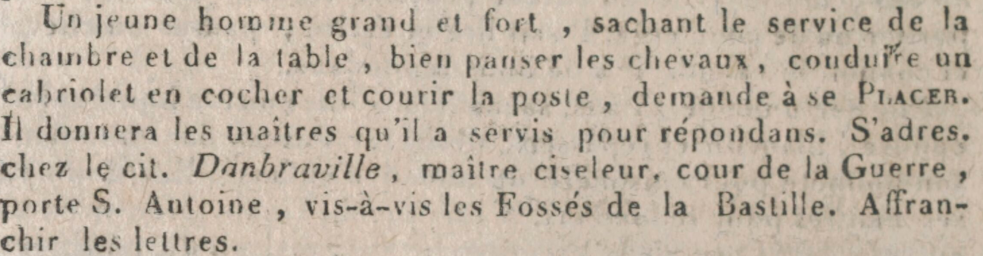
\includegraphics[width=12cm]{exemple_segmentation.png}
	\caption[Exemple d'annonce posant problème lors de la segmentation]{Exemple d'annonce posant problème lors de la segmentation: la première expression régulière coupe l'annonce en trois (après "PLACER." et après "S'adres."); la nouvelle expression régulière ne permet pas de pallier au problème de la première coupure, mais permet de contourner la seconde (\textit{Affiches de Paris}, 24 février 1804, p.8).}
\end{figure}

\begin{figure}[ht]
	\centering
	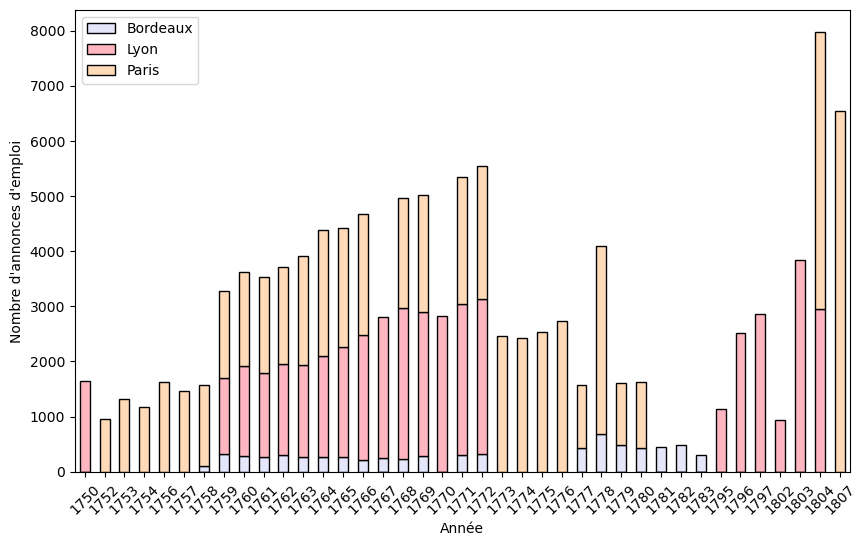
\includegraphics[width=12cm]{nb_annonces_tout_par_ville.png}
	\caption{Nombre d'annonces publiées par an selon la ville}
\end{figure}



\section{Des annonces aux annonces d'emploi: le processus de sélection}

Une fois les annonces isolées, il s'agissait ensuite de sélectionner parmi elles uniquement les annonces d'emploi. Pour ce faire, j'ai encore une fois privilégié l'usage d'une expression régulière. Après avoir lu plusieurs dizaines d'annonces, aussi bien dans les éditions parisiennes, bordelaises que lyonnaises des \textit{Affiches}, j'ai observé que la présence des expressions « se placer », « être placé » ou « une place » est le critère le plus déterminant dans la classification entre les annonces d’emploi et les autres annonces. D'où l'expression régulière suivante : \fbox{(une|être|se) place?é?r?"}. Après plusieurs tests, j'ai également observé que cette méthode incluait beaucoup d'annonces de voyages ou de ventes de voitures ("On offre une place dans une chaise de poste...", "On vend un cabriolet à une place..."); j'ai alors défini une expression spécifique pour en exclure une partie du corpus final.


\begin{figure}[ht]
	\centering
	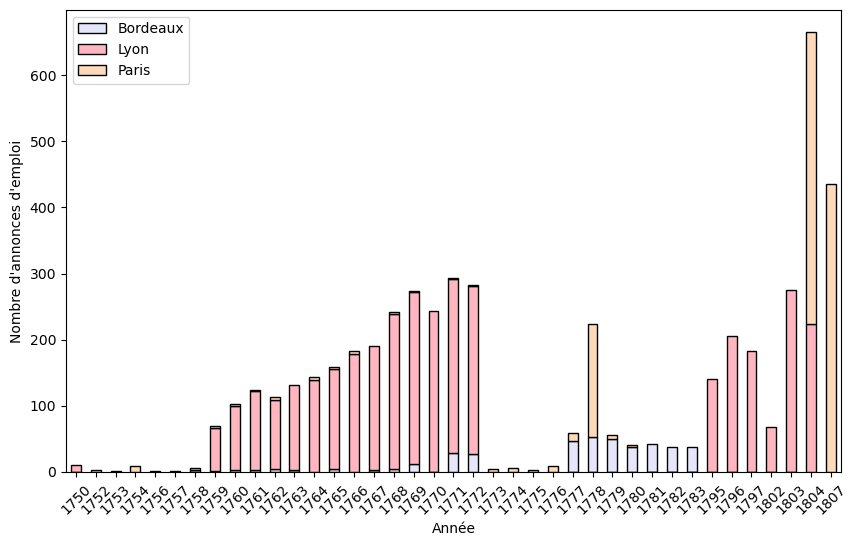
\includegraphics[width=12cm]{nb_annonces_emploi_par_ville.png}
	\caption{Nombre d'annonces d'emploi publiées par an selon la ville}
\end{figure}


\section{Des annonces d'emploi au  \textit{dataframe}: le choix du mode de stockage des données}

La méthode que j'ai décrit jusqu'ici a permis d'extraire 5064 annonces d'emploi à partir des journaux numérisés. Une dernière étape de la constitution du corpus consistait à choisir le meilleur format de stockage des annonces. Afin de préserver le maximum de métadonnées (date, ville de publication, ...), j'ai choisi de les stocker sous forme de \textit{dataframe pandas}, c'est-à-dire de tableau à deux dimensions. Le corpus initial prend donc la forme d'un tableau dont les colonnes sont: la ville de publication, l'année, le mois et le jour de publication, le texte de l'annonce. 
À partir de ce premier \textit{dataframe}, j'ai pu effectuer quelques traitements à l'aide de spacy et ajouter plusieurs colonnes: texte lemmatisé, texte sans mots vides, longueur. Ce examen initial des annonces a permis de produire de premiers résultats, limités mais qui donnent une vue d'ensemble du corpus. 

J'ai tout d'abord extrait les lemmes les plus fréquents du corpus, qui montrent bien l'uniformité des annonces entre elles: la présence de "adresser" dans plus de quatre annonces sur cinq, de "demande" et "désire" dans plus d'une sur trois, sont autant d'indices qui impliquent l'existence d'un script formel employé par le journal au moment du recueillement de la demande d'emploi. 

\begin{table}[ht]
	\parbox{.45\linewidth}{
		\centering
		\begin{tabular}{lc}
			\hline
			\multicolumn{1}{c}{\textbf{Lemme}} & \multicolumn{1}{c}{\textbf{Occurrences}} \\ \hline
			adresser                           & 4407                                      \\
			place                              & 3245                                      \\
			rue                                & 3167                                      \\
			placer                             & 2672                                      \\
			bon                                & 2510                                      \\
			maison                             & 1780                                      \\ 
			homme                              & 1780                                      \\ 
			demande                            & 1701                                      \\ 
			désirer                            & 1640                                      \\ 
			trouver                            & 1586                                      \\ \hline
		\end{tabular}
	}
	\hfill
	\parbox{.45\linewidth}{
		\centering
		\begin{tabular}{lc}
			\hline
			\multicolumn{1}{c}{\textbf{Lemme}} & \multicolumn{1}{c}{\textbf{Occurrences}} \\ \hline
			jeune                              & 1498                                      \\ 
			faire                              & 1485                                      \\ 
			donner                             & 1422                                      \\ 
			bien                               & 1307                                      \\ 
			écrire                             & 1277                                      \\ 
			ville                              & 1108                                      \\ 
			qualité                            & 989                                       \\ 
			degré                              & 914                                       \\ 
			entendre                           & 906                                       \\ 
			femme                              & 869                                       \\   \hline
		\end{tabular}
	}
	\caption{Vingt mots les plus fréquents du corpus lemmatisé et sans stopwords}
\end{table}


\begin{figure}[h]
	\centering
	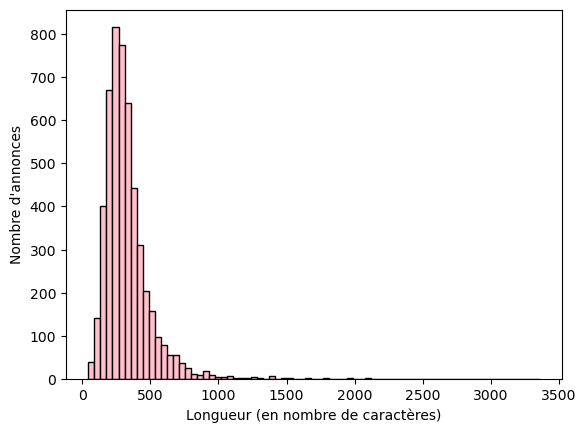
\includegraphics[width=12cm]{longueur.png}
	\caption{Répartition des annonces selon leur longueur}
\end{figure}

J'ai également pu à partir de ce premier dataframe m'intéresser à la longueur des annonces. Celle-ci est très homogène: plus de trois annonces sur quatre font entre 200 et 400 caractères, avec une médiane à 292 caractères. La norme formelle de l'annonce s'accompagne donc d'une norme de longueur, la petite annonce étant caractérisée par une brièveté qui garantit aussi la rentabilité du modèle des \textit{Affiches}.

Enfin, je souhaitais également m'intéresser lors des explorations préliminaires du corpus au phénomène de répétition et de republication des annonces, qui m'était apparu comme relativement important lors de mes lectures proches des journaux. Face à la gratuité de la publication, rien n'empêche de fait les domestiques en recherche d'emploi de proposer plusieurs fois leurs services dans plusieurs numéros différents, surtout si leur première demande s'est soldée par un échec. Néanmoins, la recherche automatique des annonces "doublons", grâce à la fonction "duplicated" de la librairie pandas appliquée aux annonces nettoyées, n'a pas portée ses fruits: seules 74 annonces sont extraites. Ces dernières sont pour la plupart republiées une seule fois; quelques annonces isolées sont répétées trois ou quatre fois, le plus souvent dans des numéros adjacents, ou dans le même mois. Des micro-variations typographiques, déjà présentes entre les annonces ou résultant de l'océrisation, expliquent probablement cette impossibilité d'extraire plus d'annonces répétées. Une autre solution, que je n'ai pas exploré ici, aurait pu être de s'intéresser à la répétition des adresses, seule partie de l'annonce qui est a priori garantie de ne pas être modifiée.
	\part{"Jeune fille de province", "garçon" et "veuve d'âge mûr": une première approche socio-démographique des annonces}



\chapter{Femmes et hommes des petites annonces}

L'un des grands chantiers de l'historiographie du travail domestique à l'époque moderne a été d'établir le profil socio-démographique du groupe des travailleuses et travailleurs ancillaires, une tâche compliquée à la fois par la taille de ce groupe dans les grandes villes et leur présence très limitée dans les sources. Néanmoins, certains consensus existent: si la domesticité dans son ensemble est plutôt mixte, les employées de la "petite domesticité", qui concerne la grande majorité de la population, sont surtout des femmes, jeunes et non-mariées, souvent issues de la ruralité, et pour qui le statut de domestique est transitoire au moment de l'arrivée en ville. Ce profil ne doit cependant pas faire oublier la diversité interne à la domesticité, qui se manifeste notamment pour certains postes très particuliers car très qualifiés (secrétaires, hommes d'affaires, ...) ou dans les très grandes maisons. Dans ces cas, le genre du service tend à s'inverser et, de manière générale au XVIIIè siècle, plus on s'approche du haut de la hiérarchie ancillaire, plus la domesticité est masculine. Ainsi, Jacqueline Sabattier établit à partir du dépouillement d'insinuations testamentaires parisiennes de la fin du XVIIIè siècle que 54\% des domestiques sont des hommes, 46\% des femmes. Elle montre également que les femmes sont omniprésentes dans les maisons à moins de quatre domestiques, mais minoritaires et cantonnées aux rôles les moins rémunérés dans les maisons avec une domesticité importante. Par ailleurs, elle observe une augmentation de la petite domesticité féminine et une masculinisation croissante de la grande domesticité au cours du siècle; en clair, une division sexuée du travail de plus en plus marquée.

Qu'en est-il des domestiques des petites annonces? Dans quelle mesure les demandeurs et demandeuses d'emploi dans la presse correspondent-ils à cette démographie? Comment expliquer les éventuelles disparités entre ce groupe particulier et la population générale? À travers une analyse du sexe, de l'âge, de l'origine et de la situation déclarée des rédacteurs et rédactrices, il s'agit d'interroger la représentativité des annonces domestiques. 


\section{Méthode}

Après constitution du corpus, une première méthode exploratoire a consisté en la recherche basique des tokens "femme" et "homme" dans les textes, en vue d'obtenir un premier aperçu de la répartition genrée des annonces. Cette première méthode a permis d'extraire le genre de 2154 annonces (sur un total de 5064): 1451 hommes et 703 femmes. Évidemment, cette méthode comprend de nombreuses limites: elle ne prend pas en compte la diversité des qualificatifs employés dans les annonces (et qui sont particulièrement variés pour les femmes: fille, dame, veuve, demoiselle, ...). De plus, elle se base sur l'intégralité du texte de l'annonce, alors que les informations genrées sur le demandeur ou la demandeuse se concentrent au début de l'annonce; la présence du mot "homme" ou "femme" plus loin dans le texte n'est pas significative. 

\begin{figure}[h]
	\centering
	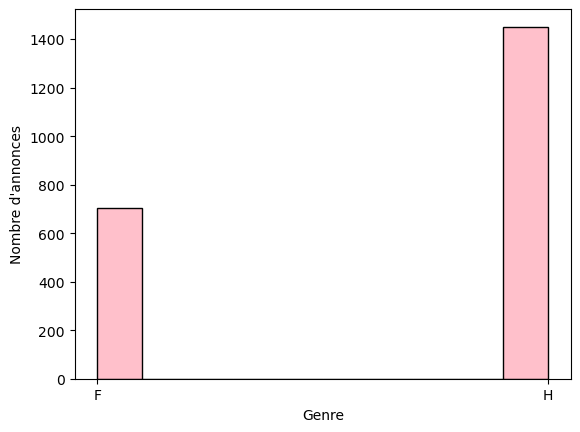
\includegraphics[width=12cm]{hist_genre_explo.png}
	\caption{Répartition des annonces selon le genre (méthode 1)}
\end{figure}


Ainsi, l'observation des limites de cette première méthode a mené à l'élaboration d'un script plus abouti pour extraire les informations liées au sexe de l'annonce: ce script sélectionne tout d'abord les cinq premiers mots de l'annonce (afin d'éviter la prise en compte de mots non significatifs, comme dans "un jeune homme de province, sans femme ni enfants"), avant d'extraire à l'aide d'expressions régulières certains qualificatifs de genre, dont la liste a été établie et amendée sur la base d'une lecture proche des annonces. Pour les annonces "masculines", ces qualificatifs sont: "homme", "garçon", "citoyen", "particulier", "sieur". Pour les femmes, il s'agit de : "femme", "fille", "dame", "demoiselle", "particulière", "veuve", "citoyenne". Les adjectifs "nommé" et "nommée" permettent d'inclure les annonces où les demandeuses et demandeurs sont appelés par leur nom ("Le nommé François..."). De plus, une dernière catégorie, "Personne", a été ajoutée pour les cas (nombreux) où l'annonce débute par "Une personne cherche..." ou, le plus souvent, "Une jeune personne cherche...". Si, dans le vocable du XVIIIè siècle, une "jeune personne" désigne plus souvent une jeune femme, j'ai tout de même préféré laisser ces cas de côté, en l'attente d'autres éléments de l'annonce qui permettraient de genrer celle-ci plus finement. 


\begin{table}[h]
	\centering
		\begin{tabular}{cclcc}
			\hline
			\textbf{Ville} & \textbf{Date} & \multicolumn{1}{c}{\textbf{Annonces}}                                                                                                                                                                                                                                                                        & \multicolumn{1}{c}{\textbf{Genre}} & \multicolumn{1}{c}{\textbf{Qualif. de genre}} \\ \hline
			Lyon           & 1802-10-09            & Une Veuve d'un âge mûr (...) & F                         & veuve                                      \\ 
			Lyon           & 1804-01-07        & Un Homme au fait du service (...)                                                                                                          & H                         & homme                                    \\ 
			Paris          & 1807-05-29      & Une personne âgée de 36 ans (...)                                                                                                        & Personne                  & personne                                  \\ \hline
		\end{tabular}
	\caption{Aperçu du \textit{dataframe} après extraction des informations genrées}
\end{table}

\section{Des annonces plutôt masculines, mais qui se féminisent lentement}

Avec cette deuxième méthode, il devient possible de définir le genre de 3611 annonces. Les annonces semblent demeurer en majorité écrites par des hommes:  1882 contiennent des qualificatifs masculins, contre 1045 pour les qualificatifs féminins. Néanmoins, l'hypothèse selon laquelle les annonces commençant par "une personne" (684 annonces) seraient plutôt féminines tendrait à relativiser ce constat et à rééquilibrer le \textit{sex ratio} du corpus. Les annonces dites "indéterminées" (c'est-à-dire celles pour lequelles on n'a pas pu aboutir à une classification femme ou homme) le sont pour diverses raisons: problèmes d'océrisation qui n'ont pas été corrigées ("Une jeune personné (sic) de 28 à 29 ans..."), problèmes de segmentation, usage de qualificatifs de métiers plutôt que de genre ("Un teneur de livres...", "Un jardinier...", "Deux frères..."). Enfin, cette approche ne fonctionne que dans les cas d'annonces de demandes d'emploi; les annonces d'employeurs, dont la forme est plus variée mais qui commencent souvent par "On desireroit trouver" ou "On cherche", nécessiteraient une autre méthode. 

Étant donné l'historiographie de la domesticité que j'ai évoquée plus haut, et selon laquelle femmes et hommes se répartissent différemment dans l'espace de la domesticité, ces résultats peuvent donner lieu à deux pistes d'interprétations. 
Première interprétation possible: les annonces sont plus employées par les hommes de manière générale, issus de la petite comme de la grande domesticité. La (légère) disparité entre annonces masculines et féminines s'expliquerait alors par un recours sexuellement différencié à ce support, qui pourrait s'expliquer de plusieurs façons: taux d'alphabétisation plus élevé pour les hommes au XVIIIè siècle \footcites{queniartEtapesResultatsProcessus1998} (bien que l'énonciation de l'annonce au Bureau d'adresses se fasse à l'oral, on peut supposer qu'il perdure un rapport différent à l'écrit), réseaux d'information différents quant à la recherche d'emploi. 
Deuxième interprétation: les annonces sont un support privilégié par la grande domesticité qualifiée, et délaissée, ou moins utilisée, par la petite et moyenne domesticité pourtant majoritaire dans la population générale, ce qui expliquerait ce déséquilibre. C'est l'hypothèse privilégiée par Ulrike Krampl qui, dans son dépouillement des\textit{ Affiches} entre 1760 et 1788, ne relève qu'un tiers d'annonces féminines\footcites{kramplPresseAnnoncesParisienne2020}.

\begin{figure}[h]
	\centering
	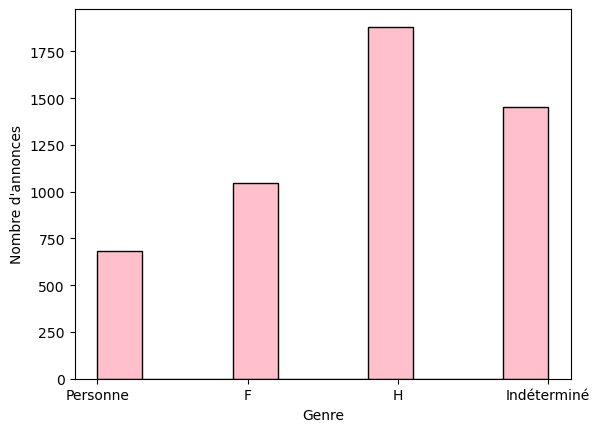
\includegraphics[width=12cm]{hist_genre.png}
	\caption{Répartition des annonces selon le genre (méthode 2)}
\end{figure}

En outre, l'analyse de la variable de genre dans le temps révèle un \textit{sex ratio} relativement stable: les annonces marquées comme masculines restent majoritaires des années 1750 jusqu'à la fin du siècle. Le changement le plus notable est l'apparition du qualificatif "personne" au début des années 1800 qui, si on l'interprète comme une marque du féminin, renverserait le genre des annonces en faveur des femmes: les annonces de femmes et de "jeunes personnes" constituent deux tiers des annonces d'emploi publiées en 1804, et près de trois quarts en 1807. Signe avant-coureur de la féminisation (ou de la démasculinisation) de la domesticité au XIXè siècle, hasard éditorial ou usage plus mixte du support de presse, qui se massifie durant cette période? Sans analyse des annonces sur une temporalité plus longue et avec un corpus plus exhaustif, il paraît difficile de conclure. 

\begin{figure}[h]
	\centering
	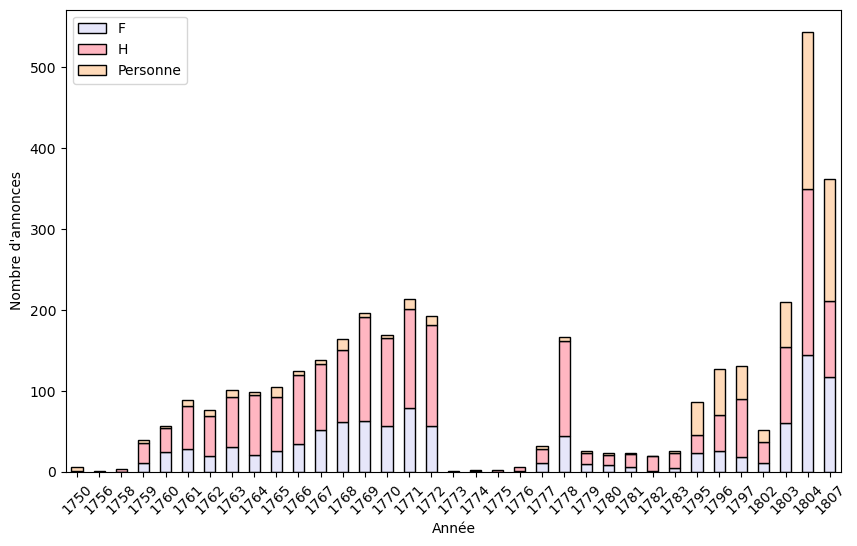
\includegraphics[width=12cm]{hist_genre_chrono.png}
	\caption{Répartition du genre des annonces dans le temps}
\end{figure}



\section{Des qualificatifs révélateurs du sexe mais également du statut social et matrimonial des demandeuses d'emploi}

Peut-être plus encore que la simple analyse sexuée des demandeurs d'emploi, l'analyse des mots employés dans les annonces pour désigner et donc assigner les individus à une catégorie sexuée est révélatrice du projet éditorial et du contexte politique de publication des \textit{Affiches}. Première observation: les qualificatifs féminins sont plus variés et révèlent davantage un statut social (d'âge, de matrimonie) que dans le cas des hommes. Là où les termes masculins emploient en grande majorité "homme" ou "garçon" (87\% des annonces d'hommes), les annonces féminines se répartissent entre "femme", "fille", "demoiselle", "mademoiselle", "dame" et "veuve". Ces qualificatifs renseignent non seulement sur le sexe de la demandeuse d'emploi, mais également sur son statut social et matrimonial, une information particulièrement importante pour les employeurs potentiels. En effet, si les hommes sont nombreux à être mariés parmi les domestiques du XVIIIè siècle, les femmes servantes représentent au contraire une population très majoritairement célibataire\footcites[p.79]{mazaServantsMastersEighteenthcentury1983}, et ce pour plusieurs raisons. Tout d'abord, la domesticité féminine est une condition souvent passagère, que les jeunes femmes exercent dans l'optique de se constituer une dot puis de s'établir. En outre, le célibat, ou en tout cas l'absence d'un mariage et d'une famille, est un critère d'employabilité important pour les femmes: si un homme marié peut continuer sans trop d'encombres à être valet, jockey ou régisseur, le mariage signifie immanquablement la fin du service domestique pour les femmes, notamment parce que les textes normatifs et législatifs de l'Ancien Régime réprouvent et stigmatisent l'emploi de servantes mariées\footcites[p.78]{mazaServantsMastersEighteenthcentury1983}. Dans ce contexte, la présence massive des qualificatifs "demoiselle" et "fille" dans les annonces peut être considérée comme une stratégie d'emploi, visant à se mettre en conformité avec l'idée que les maîtres et maîtresses se font de "la bonne domestique" au XVIIIè siècle.

Plus tard, la Révolution française introduit l'usage de "citoyen" et "citoyenne", termes à portée égalisatrice qui omettent volontairement la position sociale ou d'âge; c'est également le cas de "personne", dont l'usage augmente significativement à la fin du siècle (plus de 40\% des annonces publiées entre 1795 et 1807). Néanmoins, les lacunes du corpus dans les premières années révolutionnaires empêchent de véritablement mesurer leur apparition. 


\begin{table}[ht]
	\centering
		\begin{tabular}{lc}
			\hline
			\multicolumn{1}{c}{\textbf{Qualificatif de genre}} & \textbf{Occurrences} \\ \hline
			homme                                                & 1193            \\ 
			personne                                             & 684             \\ 
			garçon                                               & 448             \\ 
			fille                                                & 362             \\ 
			femme                                                & 258             \\ 
			(ma)demoiselle                                       & 211             \\ 
			particulier                                          & 187             \\ 
			veuve                                                & 128             \\ 
			dame                                                 & 74              \\ 
			sieur                                                & 26              \\ 
			citoyen                                              & 23              \\ 
			nommé                                                & 11              \\ 
			citoyenne                                            & 8               \\ 
			nommée                                               & 1               \\ \hline
		\end{tabular}
		\caption{Fréquence des différents qualificatifs sexués dans le corpus}
\end{table}


\begin{figure}[t]
	\centering
	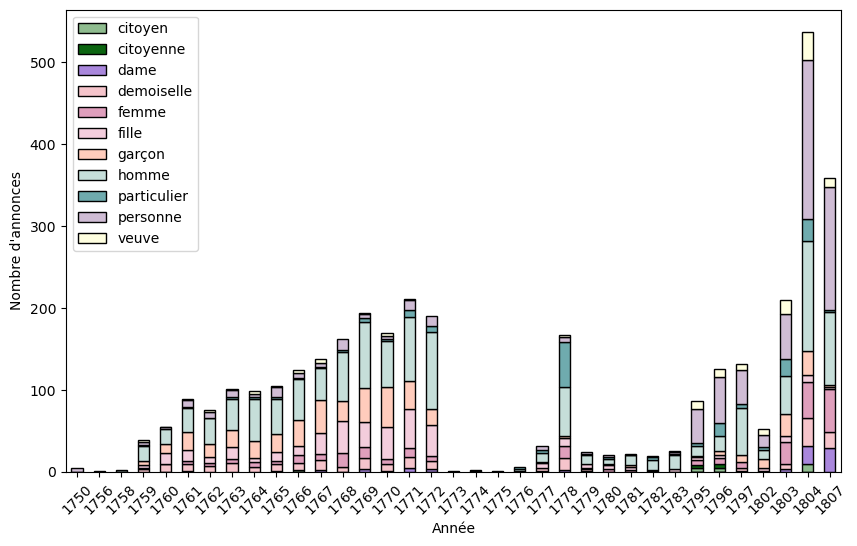
\includegraphics[width=12cm]{hist_qualif_genre_chrono.png}
	\caption{Répartition des qualificatifs sexués dans le temps}
\end{figure}



\chapter{La domesticité, une affaire de jeunesse?}

Si la domesticité concerne une part non négligeable de la population des trois villes étudiées, elle ne se répartit pas également dans l'espace social; l'un des apports de l'histoire démographique a notamment été de définir l'état ancillaire comme une étape du parcours de vie des individus, qui commence à l'adolescence et prend généralement fin avec le mariage, entre 25 et 30 ans au XVIIIè siècle\footcites{chamouxDomesticiteParcoursVie2009}. La condition domestique est donc majoritairement une condition de jeunesse, une condition transitoire censée attirer de très jeunes gens souhaitant s'établir en ville.

Qu'en est-il des petites annonces? Dans quelle mesure reflètent-elles cette réalité, ou s'en éloignent-elles? 



\section{Méthode}

Comme pour la variable de genre, l'extraction de l'âge des annonces s'est principalement faite sur la base d'expressions régulières. 

L'expression employée, \fbox{"(\textbackslash{w}+-?\textbackslash{w}*?) an(née)?s"} permet à la fois d'extraire les âges écrits en lettres ("vingt-quatre ans") et en chiffres ("32 années"). Puis, une librairie Python spécifique, text2num, a permis de transformer et d'harmoniser tous les résultats extraits en chiffres, afin de permettre des traitements quantitatifs. Cette méthode permet ainsi d'assigner un âge à 1256 annonces. 

Bien que ce nombre représente moins d'un tiers de annonces, cela ne signifie pas forcément que la méthode d'extraction est défectueuse; en effet, une lecture proche préalables des annonces a permis d'observer que l'âge est une information peu donnée par les domestiques. Plusieurs raisons peuvent expliquer cette absence: l'âge n'est pas (encore) un élément central de définition de l'individu à l'ère pré-statique, où l'enregistrement paroissial ou gouvernemental des naissances n'est pas généralisé\footcites{rennesAge2016}; il n'est pas rare de ne pas connaître son âge exact, et plusieurs annonces mentionnent d'ailleurs un âge approximatif ("autour de" ou "d'environ vingt-ans"). Avant le XIXè siècle, plus qu'un âge numérique exact, c'est surtout le positionnement dans un "âge de la vie" qui a cours\footcites{schmittInventionAnniversaire2007}: ainsi, la présence de qualificatifs ("jeune", "d'un âge mûr"...), moins précis mais qui pointent malgré tout vers une certaine période de l'existence, est commune dans les annonces. Certains exemples, qui cumulent position d'âge et de genre, ont déjà été évoqués (demoiselle, fille, garçon...). D'autres (jeunes, d'âge mûr, d'âge avancé, ...)ont pu être extraits à l'aide d'expressions régulières simples appliquées au début des annonces. Au final, 1391 annonces contiennent au moins un de ces qualificatifs;  la grande majorité (1066) contiennent l'adjectif "jeune". 
Si l'on comptabilise les annonces qui évoquent soit un âge numérique, soit un qualificatif d'âge, ce sont donc 1519 annonces qui contiennent une information relative à l'âge du demandeur ou de la demandeuse d'emploi.

Pour expliquer ce chiffre qui reste relativement bas, il faut envisager la possibilité que la mention de l'âge ne soit peut-être pas considérée comme un critère primordial de la recherche d'emploi, aussi bien pour les domestiques que pour les employeurs ou les rédacteurs du Bureau d'adresses. Si la jeunesse semble être une qualité valorisée, puisqu'une annonce sur cinq la mentionne, l'âge exact ou même imprécis ne semble pas être indispensable à l'embauche. Malgré ces éléments qui tendraient à relativiser l'importance de cette variable pour l'étude du corpus, que peut-elle nous apprendre sur la domesticité des \textit{Affiches}?


\section{Des annonces globalement jeunes, mais plus âgées que la norme domestique}

Les âges qui ont pu être extraits des annonces vont de 10 à 60 ans, mais sont très inégalement répartis: plus de 75\% des demandeurs et demandeuses ont entre 20 et 40 ans; l'usage des annonces semble assez limité pour les moins de 20 ans et les plus de 50 ans. Ces résultats vont dans le sens de la littérature et des données démographiques déjà évoquées: les jeunes adultes sont surreprésentés parmi la domesticité urbaine. 

Mais une observation plus fine de la répartition des âges permet de relativiser légèrement ce constat, et de noter une spécificité des annonces: la moyenne comme la médiane des âges se situe autour de 30 ans, ce qui est généralement donné comme la fourchette haute des âges de la domesticité (et correspond plutôt à l'âge du mariage); or ici, 50\% des demandeurs et demandeuses ont plus de 30 ans. Pratiquement autant d'annonces mentionnent un âge compris entre 20 et 30 ans (713 annonces) qu'un âge compris entre 30 et 40 (583). 

Plusieurs raisons pourraient expliquer cette (légère) différence d'âge entre domestiques en population générale et domestiques des annonces. Encore une fois, celles-ci pourraient attirer un profil particulier de domestiques, plutôt qualifié et plus âgé, la mention d'un âge plus avancé devenant alors synonyme non pas de vieillesse mais d'expérience. Autre hypothèse: l'annonce pourrait être envisagée comme support de recherche d'emploi alternatif par des individus qui ne correspondent plus au profil-type de la domesticité (très jeune, actif), et pour qui les réseaux habituels de recrutement ne suffisent plus. 


\begin{figure}[ht]
	\centering
	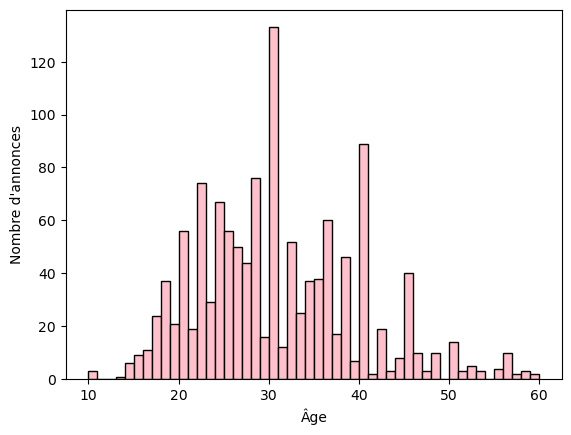
\includegraphics[width=12cm]{hist_age.png}
	\caption{Répartition des âges au sein des annonces}
\end{figure}

\begin{figure}[ht]
	\centering
	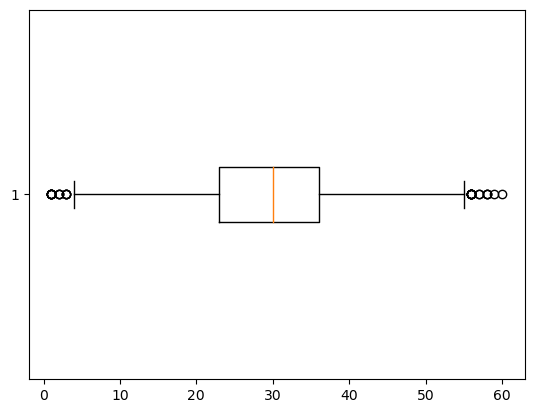
\includegraphics[width=6cm]{boxplot_age.png}
	\caption{Boîte à moustache des âges au sein des annonces}
\end{figure}



\section{Âge et genre des domestiques: des variables décorrélées}


Extraire l'âge  permet également de croiser cette information avec le genre des petites annonces. Dans la continuité de la littérature déjà évoquée, l'hypothèse la plus probable est celle de demandeuses d'emploi plus jeunes que leurs homologues masculins. 

Là-encore, néanmoins, les annonces révèlent une population distinctive, qui ne répondent pas au schéma d'une domesticité féminine jeune et d'une domesticité masculine au contraire plus âgée ou expérimentée. En effet, lorsqu'on isole les demandes féminines puis masculines, les moyennes et médianes demeurent autour de 30 ans; elles sont même légèrement plus élevés pour les femmes (autour de 32 ans), que pour les hommes. Le calcul d'un score de corrélation entre les deux variables donne un résultat très faible (-0.08), ce qui semble confirmer l'absence de relation statistique forte entre âge des genre des annonces. 

\begin{figure}[ht]
	\centering
	\begin{subfigure}[b]{0.4\textwidth}
		\centering
		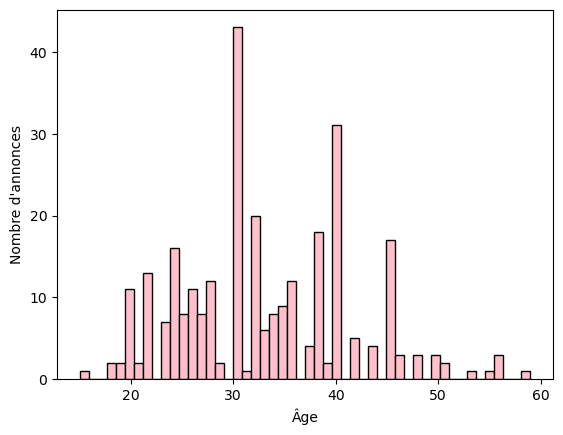
\includegraphics[width=6cm]{hist_age_F.png}
	\end{subfigure}
	\begin{subfigure}[b]{0.4\textwidth}
		\centering
		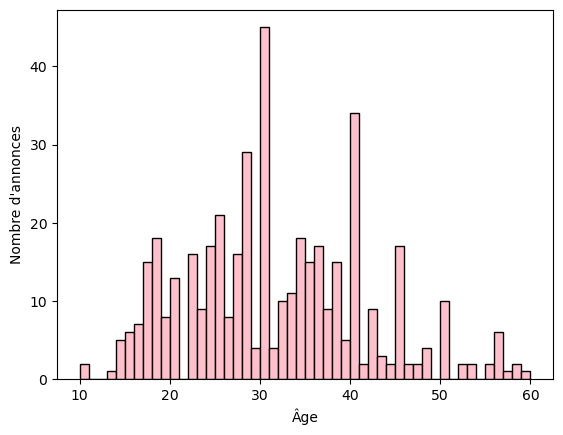
\includegraphics[width=6cm]{hist_age_H.png}
	\end{subfigure}
	\caption{Répartition des âges des annonces féminines (gauche) et masculines (droite)}
\end{figure}



En s'intéressant aux annonces qui contiennent à la fois ce qui parait être un qualificatif de sexe et d'âge ("fille", "garçon", "dame"...) et un âge numérique, on observe que ces qualificatifs ne semblent pas nécessairement refléter une position d'âge: les annonces qui contiennent les qualificatifs "garçon", "fille" et "demoiselle" ont les mêmes moyennes, médianes et répartition d'âge que l'ensemble. Ces derniers sont plus vraisemblablement des indicateurs de position ou de statut social, qui indiquent plutôt l'absence de mariage. La seule exception est le qualificatif "veuve": les demandeuses qui le mentionnent ont en moyenne 36 ans (médiane: 34 ans).



\chapter{"Arrivé des départements sans femme ni enfants": origines et situation des domestiques dans les annonces}

J'ai eu l'occasion dans les précédents chapitres de m'intéresser liminairement à la question de la position sociale et matrimoniale des demandeuses d'emploi. Cette variable, de même que l'âge et le sexe des domestiques, a beaucoup intéressé l'historiographie, qui s'accorde notamment sur l'importance du célibat au sein de la condition ancillaire \footcites{chamouxDomesticiteParcoursVie2009}. 

Un autre apport important de l'historiographie a été de mettre en évidence l'homogénéité de l'origine géographique et sociale du groupe domestique urbain: au XVIIIè comme au XVIIè ou au XVIè siècles, la grande majorité des domestiques ne sont pas originaires de la ville où ils travaillent. Jacqueline Sabattier, qui s'intéresse au cas de Paris, montre que trois domestiques de la capitale sur quatre viennent du Nord de la France, notamment de Normandie et de Picardie; parmi eux, quatre sur cinq sont issus de territoires ruraux. Parmi le reste, la majorité est née dans les campagnes périphériques du bassin parisien, ou dans des régions limitrophes (Bourgogne notamment)\footcites[p.20-25]{sabattierFigaroSonMaitre1984}. 

À partir de ces constats, que peuvent nous révéler les annonces à propos de la condition, de l'origine et du statut des domestiques? 


\section{Méthode}

Pour le statut matrimonial comme l'origine des annonces, la méthode employée a reposé principalement sur des recherches de mots-clés et d'expressions régulières dans le corpus. 

Concernant la situation matrimoniale, celle-ci n'étant pas signalé par des indices grammaticaux ou des constructions précises, j'ai constitué une liste d'expressions et de termes pouvant décrire différentes situations matrimoniales et familiales: "célibataire", "veuf" ou "veuve", "sans suite", "sans femme", "sans mari", "sans enfant", "marié(e)" ou "non marié(e). J'ai ensuite cherché ces termes dans les annonces, et les ai ajouté dans une nouvelle colonne du \textit{dataframe}.


Pour ce qui est de l'origine, j'ai extrait les ensembles de mots commençant par "arrivant de", "natif de" ou "venu de", ces expressions me semblant être les plus courantes dans le corpus pour signifier le pays ou la région de naissance des demandeurs et demandeuses. 

L'expression régulière obtenue est donc:

 \fbox{(?:arrivant | arrivée? |natif |native |venue? )(?:des |du |de )(?:(?i)\textbackslash w+)}, à partir de laquelle j'ai ajouté une nouvelle colonne au \textit{dataframe}. J'ai ensuite pu extraire plus précisément le lieu d'origine (ce qui suit "arrivant de..." donc), qui a donné lieu à une autre colonne. 


\section{Célibat domestique: la solitude comme argument de vente}

La recherche des mots-clés relatifs à la situation dans le corpus a permis d'extraire 501 annonces. Parmi elles, les qualificatifs qui se rapportent au célibat (sans enfants, sans suite...) sont très largement majoritaires (plus de 90\% des annonces extraites), notamment grâce à la présence importante de "veuve" dans le corpus (261 occurrences). 


\begin{table}[ht]
	\centering
	\begin{tabular}{lc}
		\hline
		\multicolumn{1}{c}{\textbf{Situation}} & \textbf{Occurrences} \\ \hline
		veuve                                            & 261                  \\
		veuve sans enfants                               & 72                   \\
		sans suite                                       & 46                   \\
		marié                                            & 36                   \\
		sans enfants                                     & 32                   \\
		veuve sans suite                                 & 15                   \\
		marié sans enfants                               & 10                   \\
		veuf                                             & 6                    \\
		célibataire                                      & 5                    \\
		sans femme sans enfants                          & 4                    \\
		non marié                                        & 4                    \\
		veuve célibataire                                & 3                    \\
		veuve sans enfants sans suite                    & 3                    \\
		mariée                                           & 2                    \\
		sans famille                                     & 1                    \\
		non mariée sans suite                            & 1                    \\ \hline
	\end{tabular}
	\caption{Répartition des qualificatifs de situation dans le corpus}
\end{table}

À partir d'un dixième du corpus, il est difficile de dire si les annonces sont représentatives de la population domestique générale. Néanmoins, cette omniprésence du célibat parmi les annonces qui mentionnent un statut matrimonial permet sans doute de confirmer la valorisation de la solitude domestique chez les employeurs: préciser qu'on est un ou une domestique seule, voire même insister sur cet aspect (en juxtaposant les expressions: "veuve sans enfants sans suite", "sans femme ni enfants", ...) n'a rien d'anodin dans un format de publicité de soi où chaque mot compte. 

Par ailleurs, l'observation des situations matrimoniales déclarées selon le sexe semble confirmer un acquis historiographique que j'ai déjà eu l'occasion d'évoquer: le célibat est plus valorisé (ou moins négociable) dans la domesticité féminine. Seules deux demandeuses disent être mariées, contre 46 demandeurs (dont dix "mariés sans enfants"). 

Enfin, il faut noter ici la représentation importante dans le corpus des veuves, proportionnelle à leur présence dans l'économie corporative ou domestique des villes françaises au XVIIIè siècle\footcites[p.5-18]{pellegrinVeufsVeuvesVeuvage2003}{lanzaVeuvesDansCorporations2009}.


\section{Des demandeurs principalement natifs des départements français}

La méthode employée a permis d'extraire l'origine de 71 annonces: 42 parisiennes, 27 lyonnaises et deux bordelaises. Un résultat décevant au regard de la taille du corpus, mais qui va dans le sens des observations faites lors des lectures proches des annonces: l'origine reste une information peu donnée par les domestiques. Cette absence s'explique peut-être par manque de place, ou parce que cette information est jugée peu pertinente, peu susceptible d'intéresser d'éventuels employeurs, voire dévalorisante. 

Néanmoins, les quelques dizaines d'origines qui ont pu être relevées donnent tout de même certaines informations, aussi bien relatives à la norme d'écriture des journaux qu'aux espaces et aux populations qui grossissent les rangs de la domesticité au XVIIIè siècle. Tout d'abord, l'observation des origines par ville révèlent des différences formelles importantes. Ainsi, les \textit{Affiches} de Paris emploient de manière massive l'expression, très générale, "des départements" ou "de son département", qui signifie qu'on vient d'une autre région que celle de la capitale; 30 annonces sur 42 l'utilisent. Le reste précisent des localités, souvent à l'étranger (Londres, la Suisse) ou restent plus vagues: "arrivant du Nord", "natif de province". 

Les\textit{ Affiches} de Lyon, au contraire, ont tendance à préciser le lieu d'origine: 15 annonces sur 27 mentionnent une localité précise, parmi lesquelles des villes et régions françaises proches de Lyon (Saint-Claude, Saint-Andéol-le-Château), plus éloignées (Paris,  Beaugency, Comtat, Franche-Comté, Mâcon) et des villes étrangères (Munich, Balten, Rome, Madrid). Le reste des annonces lyonnaises se répartit entre celles précisant venir "de cette Ville" (quatre annonces), "de la campagne" (deux annonces) ou de province (une annonce).

Les \textit{Affiches} de Bordeaux, si elles n'ont permis d'extraire que deux annonces contenant des origines, semblent suivre le modèle lyonnais, en indiquant précisément des localités (ici, Paris et Brest). 


Si cette méthode permet donc d'extraire en partie les origines des demandeurs et demandeuses et d'avoir un premier aperçu de la géographie de la condition domestique, elle est loin d'être exhaustive. Elle omet également le récit que certains domestiques font dans les annonces de leur parcours avant leur arrivée en ville, qui est un indicateur fort de la mobilité de travail sous l'Ancien Régime, comme par exemple dans cette annonce publiée à Lyon en mars 1770: "Un jeune homme de bonne famille, âgé de vingt ans, natif de Balten en Allemagne, qui a fait son apprentissage à Dijon, chez M. Foucherot; qui est d'un caractere doux, demande une place dans un Magasin de Draperie\footnote{\textit{Affiches de Lyon}, 29 mars 1770}". 



\bigskip

Ainsi, les annonces d'emploi, loin de pallier aux limites de la quantification de l'activité domestique, se heurtent finalement aux mêmes difficultés liées aux caractéristiques de l'ère pré-statique\footcites{fauve-chamouxSurplusUrbainFemmes1998} : des individus qui ne se définissent pas forcément par leur appartenance de sexe, encore plus rarement par leur âge. Des limites encore accentuées par la dimension déclarative des annonces, où se joue un enjeu de mise en valeur de soi, d'effacement et de dévoilement de l'information qui est bien éloignée des préoccupations de la démographie contemporaine.
	\part{Savoir-faire et savoir-être: la mise en valeur de soi et de son travail dans les annonces d’emploi}



\chapter{Au cœur des annonces, la description des compétences domestiques}

Le format de l'annonce présente plusieurs difficultés pour quiconque cherche une place de domestique: elle doit être courte, impersonnelle, répondre à une mise en forme précise qui laisse peu de place à la différenciation ou à la créativité. Mais cette "expression de soi hautement contrainte\footcites{kramplPresseAnnoncesParisienne2020}" n'empêche pas les demandeurs et demandeuses de se présenter sous leur meilleur jour: la brièveté des publications permet malgré tout de se mettre en valeur et de taire ce qui, selon des normes de genre, d'âge ou de classe, éloigne du canon domestique. Cette mise en valeur passe notamment par la description de compétences ou de qualités physiques et morales. Dans cette partie, je considère donc l'annonce comme une forme de "publicité de soi", qui justifie la place des demandes d'emploi dans l'économie générale du journal d'annonces, et les rapproche d'autres types de textes publiés par les \textit{Affiches} (publicités commerciales, annonces immobilières, ...). Ainsi, dans le journal d'annonces, "l’emploi se trouve (...) d’office placé dans une logique de consommation, qui l’apparente, sinon l’assimile à un bien à échanger\footcites{kramplAdresserClercHuissier2017}". 

À travers l'étude de ce qui représente le corps de l'annonce, de ses éléments de langage les plus courants mais également des potentielles tentatives de distinction, il s'agit donc d'interroger ce qui constitue la "bonne" domesticité aux yeux des demandeurs et donc, par extension, des employeurs potentiels. 


\section{Méthode}

Parmi les différentes composantes de l'annonce, un élément, déjà signalé par l'historiographie, apparaît central: il s'agit des compétences avancées par les demandeurs et demandeuses, qu'Ulrike Krampl désigne sous le terme de "talents". Pour extraire ces informations, plusieurs méthodes ont été envisagées.

La première, la plus simple, consistait encore une fois en l'élaboration d'expressions régulières. Une lecture proche des annonces a en effet permis d'observer que, pour une part non négligeable du corpus, les compétences se situent toujours au même endroit : entre les mots "sachant" (ou "sait") et "désire" (ou "désireroit"). Les annonces qui répondent à ce critère formel très spécifique ressemblent alors à "Une jeune fille de 18 ans, sachant coudre et repasser, désire une PLACE de domestique...". Ainsi, l'expression régulière \fbox{\b(?:sachant|sait)\b (.*?) de?é?sir} trouve une correspondance dans 922 annonces. Les compétences ainsi extraites permettent de réaliser le nuage de mots suivants, déjà parlant quant à la surreprésentation (et donc la valorisation?) de certaines activités et savoir-faire domestiques (la cuisine, la couture, mais également le fait de savoir lire et écrire):

\begin{figure}[h]
	\centering
	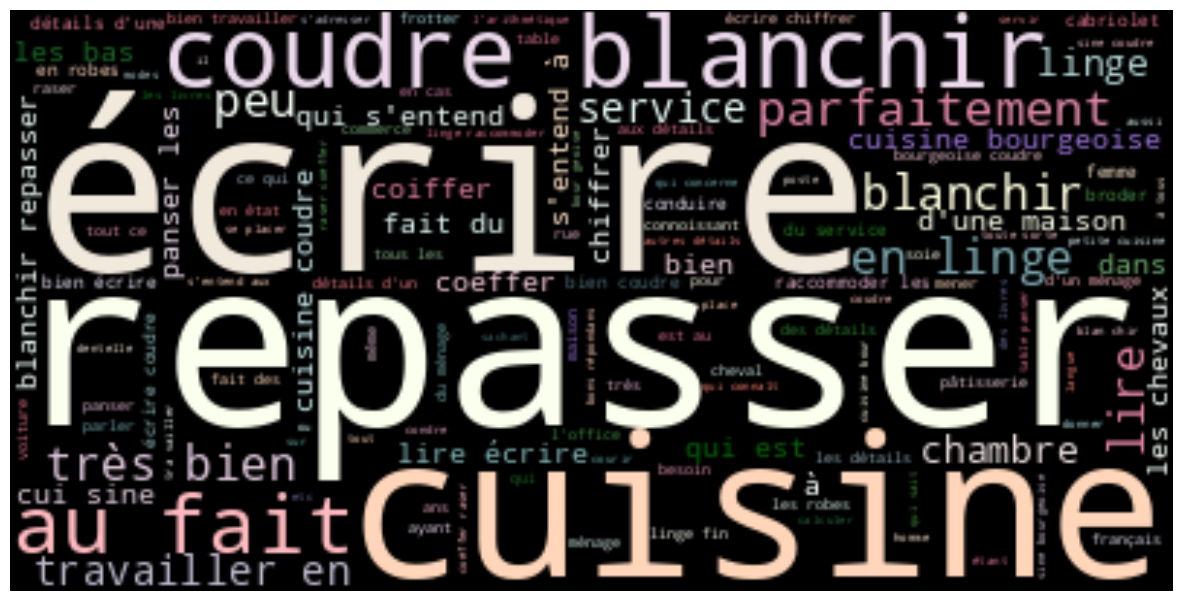
\includegraphics[width=12cm]{wordcloud_comp_regex.png}
	\caption{Nuage de mots des compétences extraites grâce aux expressions régulières}
\end{figure}

Si cette première méthode permet d'extraire les compétences avec une grande précision, elle n'est valable que pour une minorité des annonces (un cinquième du corpus). Pour les annonces ne répondant pas au modèle "...sachant [compétence], désire...", j'ai employé la librairie Spacy et sa fonction de \textit{span categorization}. Cette fonction permet, à la façon de la reconnaissance d'entités nommées (\textit{Named Entity Recognition}, ou NER), de repérer et de classer certaines parties d'un texte selon des catégories pré-définies par l'utilisateur. Néanmoins, contrairement au NER, la classification de \textit{spans} peut concerner n'importe quelle partie du texte, indépendamment de sa longueur, de sa classe ou de sa fonction grammaticale. Elle est donc plus à même de traiter des phrases ou des fragments de phrases, y compris lorsqu'ils se chevauchent. Dans notre cas, où les compétences sont signalées soit par leur place dans la structure de l'annonce, soit par certaines répétitions, cette méthode parait la plus prometteuse parmi celles proposées par Spacy.  Plus important encore ici, cette fonction est entraînable; il a donc été possible de développer un modèle propre au corpus d'annonces et à ses problématiques, sur la base d'annotations préalables. 



\newpage

\global\mdfdefinestyle{mystyle}{%
	linecolor=white,linewidth=3pt,%
	leftmargin=2cm,rightmargin=2cm
}

\begin{mdframed}[style=mystyle,frametitle={L'annotation du corpus}, backgroundcolor=LavenderBlush1] %
	
	
	Pour produire les données d'entraînement, j'ai utilisé Prodigy, un outil d'annotation disposant d'une interface en ligne et développé par l'équipe à l'origine de la librairie spacy. Pour annoter des \textit{spans}, il permet de sélectionner le texte à annoter (y compris sous forme de \textit{dataframe}), de choisir les catégories voulues (ici, compétences mais également emploi, qualités, adresse) puis de "surligner" les mots ou ensembles de mots correspondant à chaque catégorie. 	Une fois l'annotation terminée, Prodigy permet ensuite d'exporter directement les annotations au bon format et de générer automatiquement un fichier de configuration spacy. 
		
	\bigskip
	
	\centering
	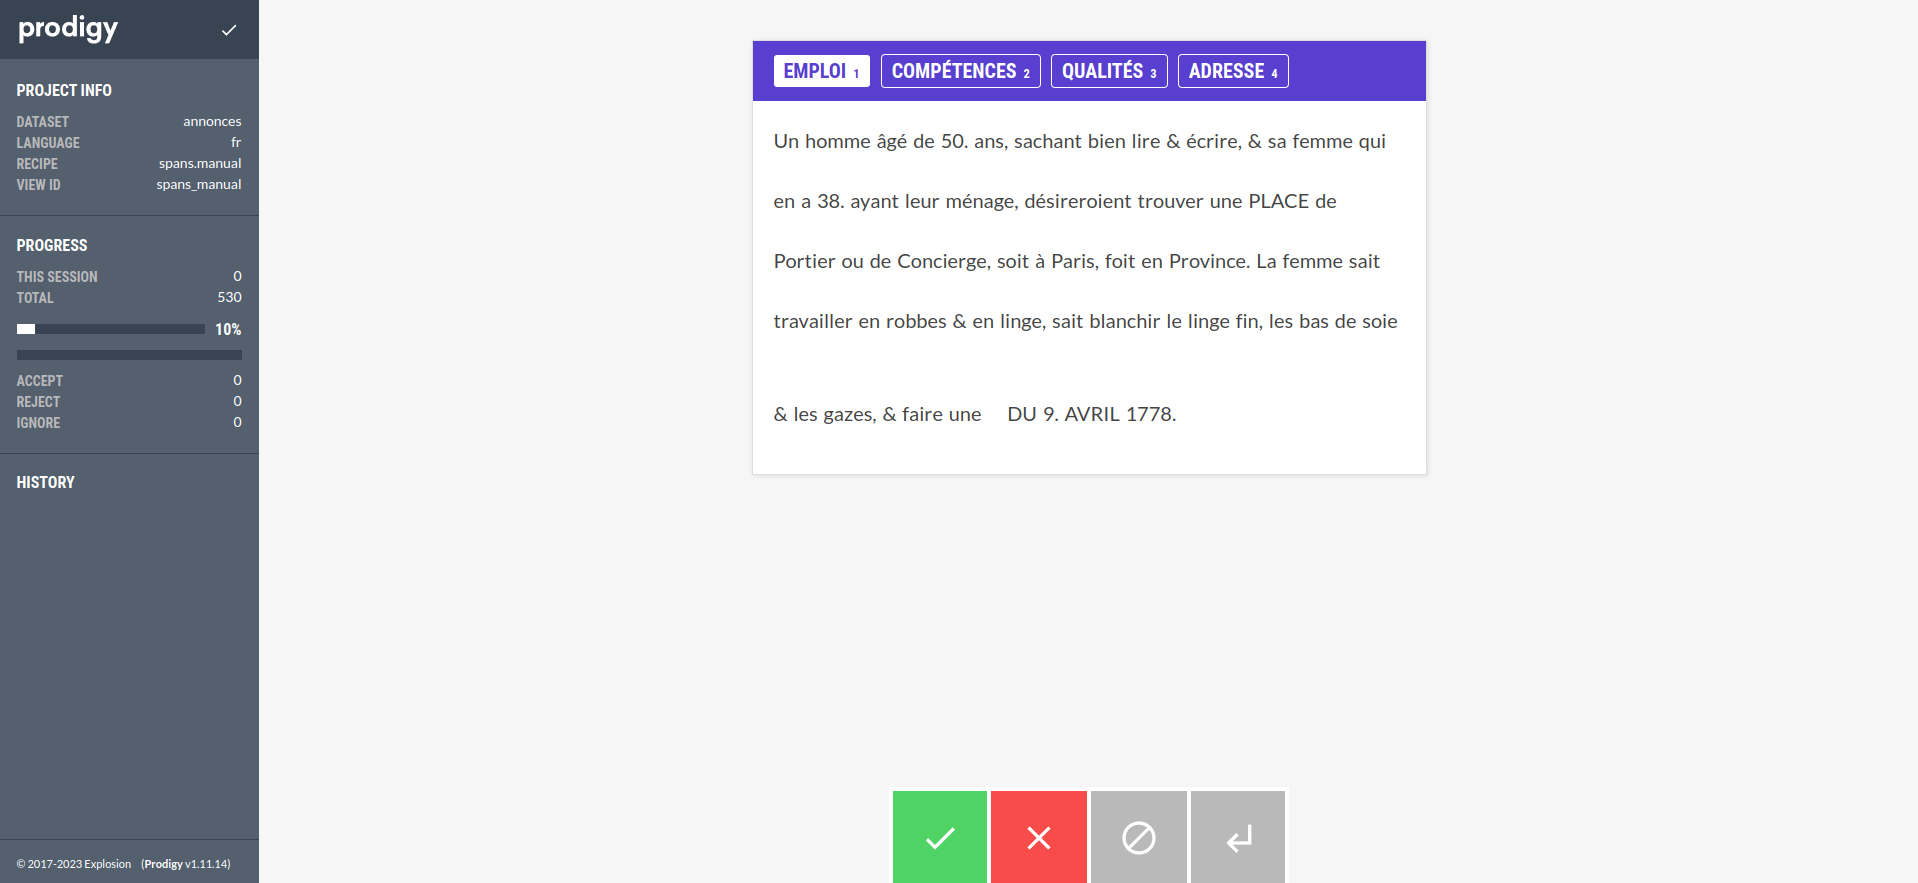
\includegraphics[width=10cm]{exemple_prodigy_1.png}
	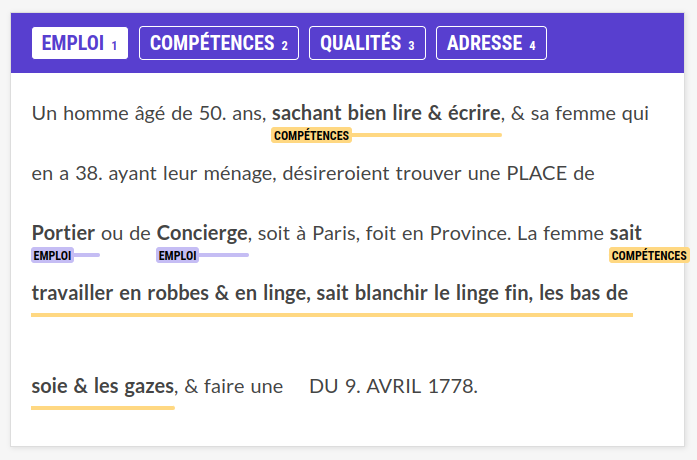
\includegraphics[width=10cm]{exemple_prodigy_2.png}
	\captionof{figure}{Exemples de l'interface Prodigy}
		
	\bigskip

		
\end{mdframed}

\bigskip

Afin de déterminer le nombre d'annonces à annoter, j'ai graduellement entraîné plusieurs modèles spacy, au fur et à mesure de l'annotation, et observé l'évolution des scores de performances du modèle en fonction du nombre d'annotation. Si les scores augmentent fortement entre la première et la 300ème annotation, ils commencent ensuite à stagner: un modèle entraîné sur la base de 300, 400 ou 500 annotations produira sensiblement les mêmes F1scores, autour de 0.6. Néanmoins, la précision (c'est-à-dire l'exactitude ou la pertinence des mots extraits et catégorisés par le modèle) est bien meilleure que le rappel (c'est-à-dire l'exhaustivité du modèle): tandis que la première se situe autour de 0.75, le second peine à dépasser 0.5. Cela signifie que le modèle, s'il parvient à bien extraire certaines compétences sans produire trop de faux positifs, n'est pas complet: il laisse de côté beaucoup d'éléments pertinents. Les compétences extraites seront donc dans leur ensemble bien des compétences, mais ne seront peut-être pas complètement représentatives; cette limite du modèle est évidemment à prendre en compte dans l'analyse.

\begin{figure}[ht]
	\centering
	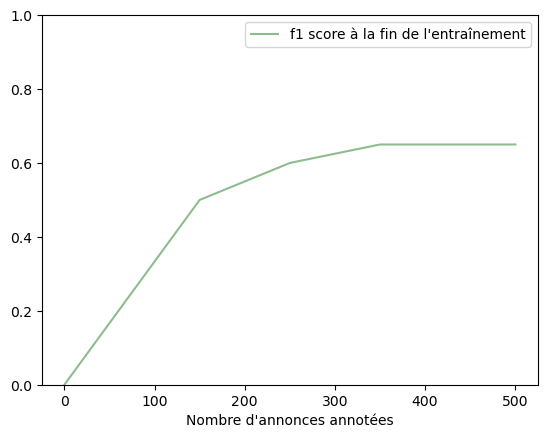
\includegraphics[width=12cm]{scores_span_cat.png}
	\caption{Évolution des scores de performance du modèle de catégorisation en fonction des annotations}
\end{figure}

\begin{figure}[ht]
	\centering
	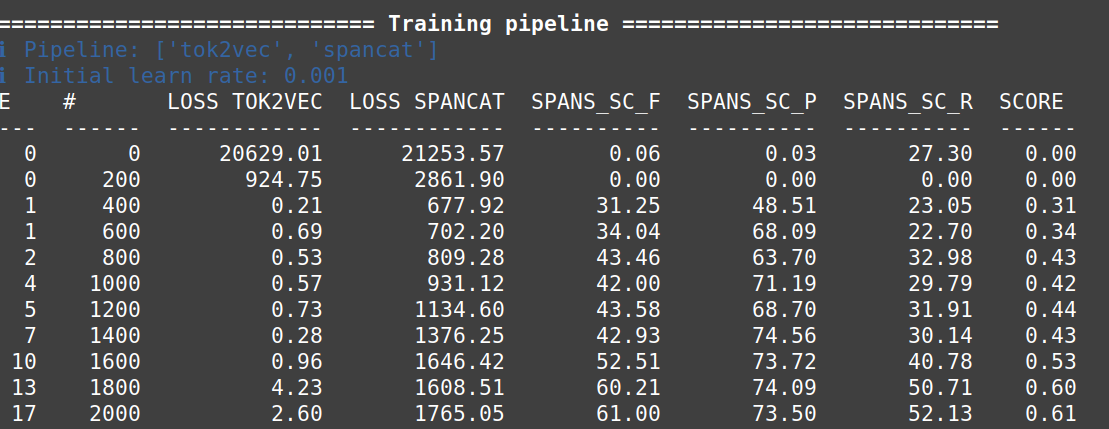
\includegraphics[width=12cm]{scores_entrainement_spacy.png}
	\caption{Évolution des scores de performance au cours de l'entraînement final}
\end{figure}

Une fois le modèle de \textit{span categorization} entraîné, une fonction a permis d'extraire les \textit{spans} catégorisés comme étant des compétences, puis d'ajouter une colonne dédiée au \textit{dataframe}. Au final, le modèle entraîné sur la base de 530 annotations permet ainsi de reconnaître 1701 annonces contenant des compétences.

\section{Lire, écrire et bien cuisiner: l'importance des verbes pour décrire des talents majoritairement manuels}

Un premier constat qui peut être fait sur la description des compétences dans les annonces est celui de l'uniformité formelle de celle-ci.  Les "talents" évoqués prennent la grande majorité du temps la forme de verbes ou d'expressions verbales ("repasser le linge", "faire une cuisine bourgeoise"). Cette caractéristique, en plus de montrer l'homogénéité éditoriale des \textit{Affiches}, fait écho à plusieurs travaux historiques, qui ont déjà montré l'importance du verbe dans la représentation et la description du travail à l'époque moderne, où l'activité des individus (notamment des femmes) est souvent plurielle et l'usage de noms de métiers encore rare. C'est notamment le cas du projet \textit{Gender and Work}, qui se base sur une méthode lexicale "orientée verbe" pour extraire automatiquement\footcites{petterssonParsingIdentificationVerb2012} les activités de sources modernes suédoises diverses (archives judiciaires, livres de compte, lettres, journaux...). Le projet s'est lui-même inspiré des travaux de Sheilagh C. Ogilvie sur l'histoire du travail des femmes en Allemagne\footcites{ogilvieBitterLivingWomen2003}. 

\begin{figure}[h]
	\centering
	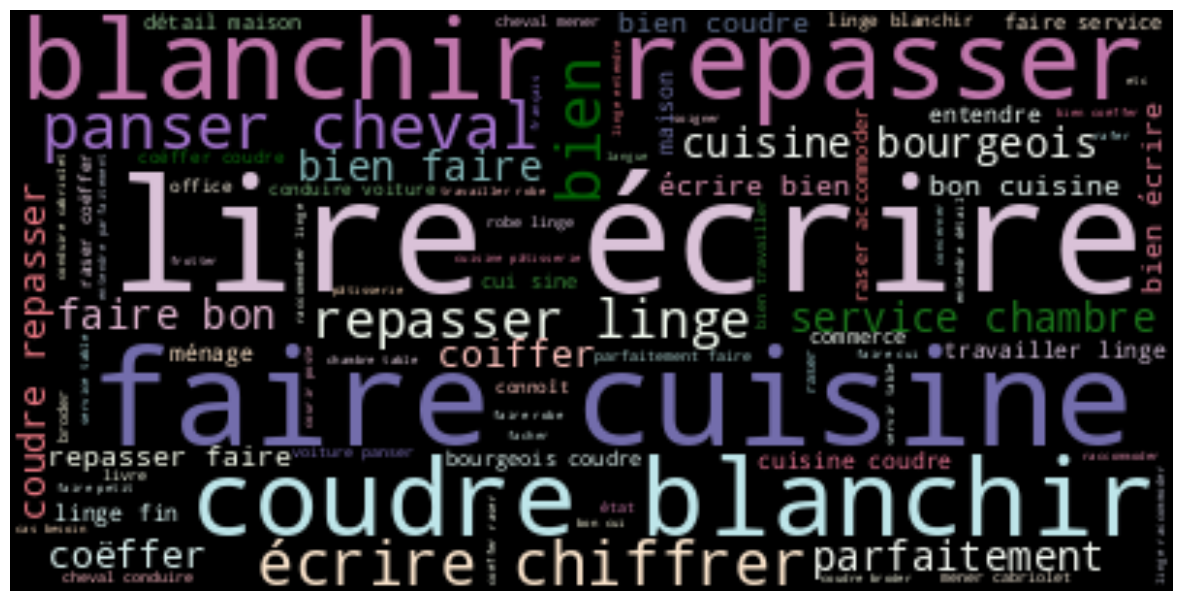
\includegraphics[width=10cm]{wordcloud_comp_spacy.png}
	\caption{Nuage de mots des compétences extraites grâce au modèle de \textit{span categorization}}
\end{figure}

Ces observations semblent se vérifier sur le corpus de petites annonces: sur 23156 tokens considérés par notre modèle comme des compétences, 5507 sont des verbes, soit plus d'un sur cinq. Sur 1701 annonces concernées, 1648 contiennent au moins un verbe de compétence; 991 en contiennent au moins trois.
De plus, l'analyse des mots les plus fréquents du corpus montre une grande uniformité des verbes employés, et donc des compétences mises en avant. L'écriture, notamment, est très valorisée: elle est présente dans près de la moitié des annonces, signe de l'alphabétisation croissante au XVIIIè siècle, mais aussi de l'avantage que cette capacité procure dans la recherche d'emploi réelle ou telle qu'elle est imaginée par les domestique. En dehors de l'écriture, de la lecture et, à une échelle moindre, du calcul, les compétences les plus réitérées sont surtout manuelles: coudre, repasser, coiffer, raser sont des aptitudes associées à une domesticité de service, aux tâches multiples dans la maison et plutôt peu qualifiée. Mais ces éléments à première vue très descriptifs sont parfois agrémentés d'adverbes ou d'adjectifs à valeur méliorative: près de la moitié des annonces contiennent au moins un adverbe, la plupart étant "bien" (492 occurrences) et "parfaitement" (179).
Certaines expressions ou ensembles de talents sont également très fréquentes, ce qui peut être observé à partir des bigrammes et trigrammes de mots: dans près d'un cas sur quatre, le mot "cuisine" fait partie de l'expression "faire une cuisine bourgeoise" (96 occurrences sur 416). Le diptyque "lire et écrire" est également très fréquent: 367 annonces mentionnent les deux compétences, 7 ne mentionnent que savoir lire et 273 mentionnent uniquement l'écriture. De même, les compétences liées au soin du linge vont souvent par paire, voire par trio: 117 annonces n'évoquent que la couture, 106 le fait de savoir "coudre et blanchir", 161 la capacité de "coudre, blanchir et repasser". 


\begin{table}[ht]
		\centering
			\begin{tabular}{lc}
			\hline
			\textbf{Mot} & \textbf{Occurrences} \\ \hline
			écrire       & 731                  \\ 
			coudre       & 508                  \\ 
			blanchir     & 480                  \\ 
			cuisine      & 441                  \\ 
			lire         & 441                  \\ 
			repasser     & 415                  \\ 
			linge        & 383                  \\ 
			coiffer      & 282                  \\ 
			service      & 210                  \\ 
			entendre     & 180                  \\ 
			cheval       & 178                  \\ 
			raser        & 161                  \\ 
			panser       & 155                  \\ 
			travailler   & 138                  \\ 
			chiffrer     & 135                  \\ 
			maison       & 126                  \\ 
			bourgeois    & 123                  \\ 
			chambre      & 118                  \\ 
			conduire     & 95                   \\ 
			ménage       & 94                   \\
			\hline
		\end{tabular}
		\caption{Vingt mots les plus fréquents parmi les compétences extraites}
\end{table}

\begin{table}[ht]
	\parbox{.45\linewidth}{
		\centering
		\begin{tabular}{lc}
			\hline
			\textbf{Bigramme} & \textbf{Occurrences} \\ \hline
			lire écrire                           & 431                  \\
			faire cuisine                         & 302                  \\
			blanchir repasser                     & 260                  \\
			coudre blanchir                       & 241                  \\
			panser cheval                         & 140                  \\
			écrire chiffrer                       & 125                  \\
			repasser linge                        & 109                  \\
			cuisine bourgeois                     & 99                   \\
			faire bon                             & 93                   \\
			service chambre                       & 85                   \\
			bien faire                            & 83                   \\
			écrire faire                          & 80                   \\
			coudre repasser                       & 75                   \\
			repasser faire                        & 75                   \\
			écrire bien                           & 73                   \\
			bien écrire                           & 72                   \\
			bien coudre                           & 69                   \\
			bon cuisine                           & 69                   \\
			travailler linge                      & 67                   \\
			cuisine coudre                        & 67                  \\
			\hline
		\end{tabular}
		\caption{Vingt bigrammes les plus fréquents}
	}
	\hfill
    \parbox{.45\linewidth}{
     	\centering
		\begin{tabular}{lc}
			\hline
			{\textbf{Trigramme}} & \textbf{Occurrences} \\ \hline
			coudre blanchir repasser               & 135                  \\
			blanchir repasser linge                & 73                   \\
			faire bon cuisine                      & 67                   \\
			lire écrire faire                      & 57                   \\
			blanchir repasser faire                & 55                   \\
			lire écrire bien                       & 54                   \\
			faire cuisine bourgeois                & 52                   \\
			bien faire cuisine                     & 51                   \\
			faire cuisine coudre                   & 48                   \\
			cuisine coudre blanchir                & 46                   \\
			bourgeois coudre blanchir              & 46                   \\
			écrire lire écrire                     & 46                   \\
			lire écrire lire                       & 43                   \\
			lire écrire chiffrer                   & 43                   \\
			repasser faire cuisine                 & 38                   \\
			cuisine bourgeois coudre               & 37                   \\
			panser cheval conduire                 & 35                   \\
			bien lire écrire                       & 35                   \\
			faire service chambre 34               & 67                   \\
			repasser linge fin                     & 32                   \\
			\hline
		\end{tabular}
		\caption{Vingts trigrammes les plus fréquents}
	}
\end{table}

\bigskip


Ainsi, une première analyse des compétences a permis de mettre en évidence l'omniprésence des savoir-faire manuels dans le corpus, et leur description majoritaire sous forme de verbes, en conformité avec l'historiographie du travail à l'époque moderne. Une seconde incursion aura pour problématique la dimension genrée de ces compétences, qui contribue à placer hommes et femmes dans des espaces différemment qualifiés de la domesticité. 

\newpage

\section{"Coudre, blanchir, repasser", "coiffer, conduire un cabriolet": des savoir-faire genrés}

Pour envisager les compétences du point de vue du genre et donc d'une potentielle division sexuée du travail, j'ai ensuite croisé les colonnes "Genre" et "Compétences", afin d'obtenir des compétences associés aux annonces de femmes d'un côté, et d'hommes de l'autre. Au final, ce sont donc 402 annonces féminines et 607 annonces masculines dont les compétences ont été extraites par le modèle, et à partir desquelles j'ai pu générer les deux nuages de mots suivants.

\begin{figure}[h]
	\centering
	\begin{subfigure}[b]{0.4\textwidth}
		\centering
		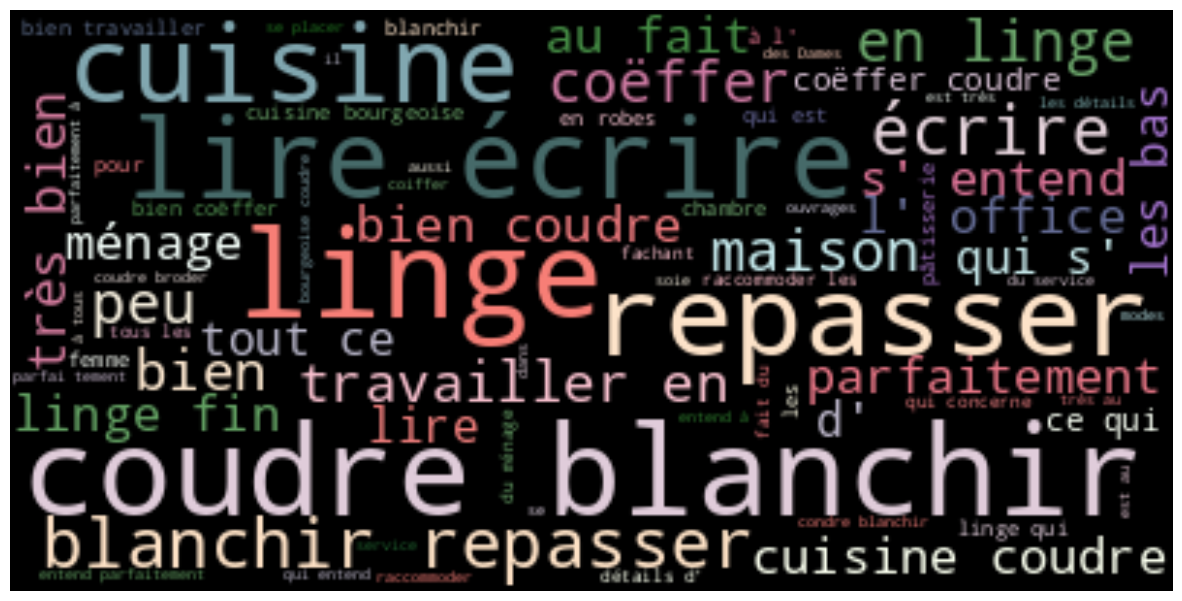
\includegraphics[width=6cm]{wordcloud_comp_F.png}
	\end{subfigure}
	\begin{subfigure}[b]{0.4\textwidth}
		\centering
		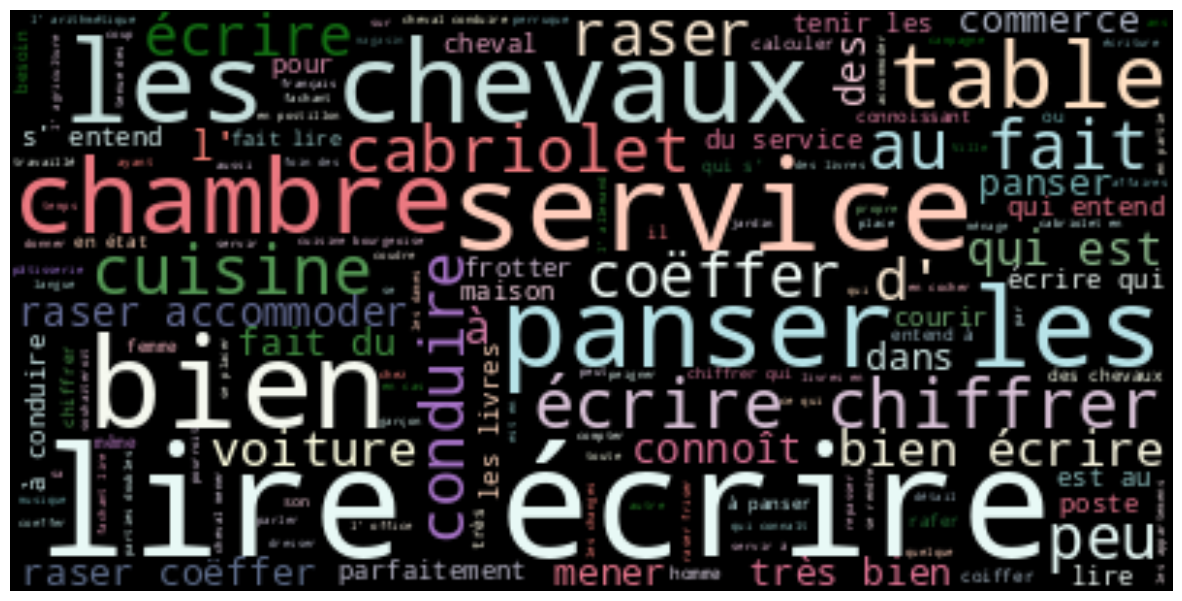
\includegraphics[width=6cm]{wordcloud_comp_H.png}
	\end{subfigure}
	\caption{Nuage de mots des compétences dans les annonces écrites par des femmes (gauche) et par des hommes (droite)}
\end{figure}


\subsection{Des compétences féminines confinées à l'intérieur du foyer}

Comme on peut l'observer à l'aide du nuage de mots ci-dessus et du tableau de fréquences suivant, les compétences féminines ont principalement trait à deux pôles d'activités: le soin du linge et la cuisine. Des activités non seulement peu qualifiées, mais surtout localisées à l'intérieur même du foyer (à l'exception notable du blanchissage, qui peut se faire à l'intérieur ou, plus couramment à Paris, sur les rives de la Seine et de la Bièvre), et qui se caractérisent par leur multiplicité: "savoir tout ce qui a trait au linge" signifie non seulement savoir le laver, le raccommoder, le repasser, mais également savoir fabriquer des pièces à la main. 

\begin{table}[ht]
	\centering
	\begin{tabular}{|l|c|}
		\multicolumn{1}{|c|}{\textbf{Mot}} & \textbf{Occurrences} \\ \hline
		blanchir                         & 203                  \\
		coudre                           & 197                  \\
		linge                            & 177                  \\
		repasser                         & 152                  \\
		écrire                           & 135                  \\
		cuisine                          & 131                  \\
		lire                             & 102                  \\
		parfaitement                     & 55                   \\
		coiffer                          & 52                   \\
		travailler                       & 48                  
	\end{tabular}
	\caption{Dix mots les plus fréquents parmi les compétences d'annonces de femmes}
\end{table}

L'omniprésence du linge parmi les compétences féminines est proportionnelle à son importance croissante dans l'économie domestique du XVIIIè siècle\footcites{rocheInventionLingeAu1986}, et au temps nécessaire à son soin durant l'ère pré-industrielle. Avoir du personnel compétent en la matière est alors essentiel: porter des chemises jaunies, servir à manger sur une nappe tâchée sont autant de fautes qui mettent en exergue la place du linge dans la "hiérarchie du paraître\footcites[p.236]{rocheInventionLingeAu1986}". À ces motifs de distinction sociale s'ajoutent également au cours du XVIIIè siècle des raisons hygiénistes\footcites{ungererValeursUrbainesPropre1986}, qui exacerbent encore l'importance d'un linge bien blanchi.

L'association des femmes à cette activité découle en grande partie de leur association plus générale au textile. La couture, notamment, devient une occupation intégralement féminine au cours des XVIIè-XVIIIè siècles, caractérisés par la perte de la main-mise de la communauté des tailleurs sur ce secteur d'activités\footcites{crowstonFabricatingWomenSeamstresses2001}{crowstonEngenderingGuildsSeamstresses2000}. Au moins jusqu'à la fin du siècle\footcites{moreraBlanchisseusesPropreBlanchisseurs2018}, le lavage du linge et les savoir-faire qui lui sont liés sont également l'apanage de femmes, qu'elles soient domestiques ou blanchisseuses spécialisées.

Au-delà des aptitudes fondamentales que constituent la couture, le blanchissage et le repassage, certaines annonces mentionnent également des compétences textiles plus rares et particulières, qui les distinguent autant qu'elles les destinent à un certain type d'employeurs: l'évocation du lavage des bas (56 occurrences), de la broderie (62) ou de certaines matières précieuses comme la soie (43) ou la dentelle (17) correspond à certains besoins et certaines demandes spécifiques des employeurs les plus fortunés.


La cuisine, quant à elle, constitue une autre activité culturellement associée à la féminité. Au XVIIIè siècle, avec l'avènement d'un savoir-vivre "à la française", qui repose en grande partie sur la gastronomie, le métier de cuisinier se masculinise, notamment dans les maisons bourgeoises et nobles où il est en vogue d'employer un "chef de haute cuisine" qui se distingue fortement du reste de la domesticité, par sa rémunération comme par son statut\footcites[p.25-35]{sabattierFigaroSonMaitre1984}. Mais dans le foyer ordinaire, la cuisine dite "de ménage" reste majoritairement une affaire de femmes\footcites{drouardChapitrePremierCuisiniers2016}. 

Comme dans le cas du linge, si sa mention dans l'annonce représente surtout un moyen de signifier la pluricompétence d'une domestique (savoir blanchir, coudre et cuisiner signale, dans la domesticité modeste, une capacité à tenir une maison seule ou presque), elle peut également prendre une valeur distinctive dès lors qu'elle s'accompagne d'adverbes ou d'adjectifs mélioratifs (faire une "très bonne cuisine" ou une cuisine "bourgeoise") voire même de spécialisations culinaires. La pâtisserie, notamment, est le vingtième talent le plus fréquent dans ce corpus féminin. 

Ainsi, dans le cas de la domesticité féminine, c'est la multiplicité des compétences et la pluri-activité qui priment: si la cuisine ou le soin du linge sont bien identifiés comme activités spécifiquement destinées aux femmes, c'est surtout l'agrégation des compétences qui valorise leur candidature, et qui les rattache au service peu qualifié, de petite maison. Les annonces de femmes sont ainsi en moyenne plus longue que les annonces d'hommes (76 mots en moyenne contre 70) et contiennent aussi plutôt plus de verbes de compétences (3,5 verbes en moyenne contre 3,1 pour les hommes). Mais c'est surtout la présence de certaines expressions englobantes, cherchant à signifier une maîtrise complète des arts de la maison, qui caractérisent les annonces de femmes, alors qu'elles sont pratiquement absentes chez leurs homologues masculins: une annonce sur cinq contient des expressions semblables à "capable de rendre tous les services pour l'intérieur d'un ménage", "très au fait de la tenue d'une maison", "sachant [...] tout ce qui concerne la manutention d'un ménage".

\subsection{Des compétences masculines tournées vers l'extérieur de la maison et le service du maître}

Les annonces masculines relèvent d'un tout autre registre. Les compétences qu'elles renferment sont, quant à elles, principalement liées au service particulier d'un maître ou à des activités de plein air et de transport. 

Les références au service personnel ont la particularité de beaucoup se référer à la pilosité: "coiffer" et "raser" sont parmi les termes les plus communs, soulignant à la fois le rôle central du valet ou du domestique particulier dans l'apparence de son maître, et l'importance d'être bien rasé durant un siècle où, pour une fraction de la population, la barbe est synonyme de déchéance sociale ou de barbarie \footcites{auzepyHistoirePoil2017}. Certaines annonces mentionnent même savoir "coiffer femmes et hommes"; si la femme de chambre est souvent chargée de coiffer sa maîtresse au quotidien, le métier ou l'art de coiffer est globalement masculin. 

Le second ensemble de compétences masculines se rapporte aux activités d'extérieur, et notamment au transport du maître: savoir conduire un cabriolet ou une voiture, s'occuper des attelages. Là encore, la fonction pratique du domestique va de pair avec une dimension ostentatoire; l'homme domestique est celui qui sort en ville et accompagne son maître partout où il va. L'importance du cheval dans les annonces est proportionnelle à l'importance de celui-ci dans la ville: élément de distinction par rapport au peuple qui va à pied, il devient progressivement indispensable aux déplacements et donc à la vie sociale des maîtres sous l'Ancien Régime\footcites{rocheCultureEquestreOccidentale2008}. 


\begin{table}[ht]
	\centering
	\begin{tabular}{|l|c|}
		\multicolumn{1}{|c|}{\textbf{Mot}} & \textbf{Occurrences} \\ \hline
		écrire                           & 342                  \\
		lire                             & 218                  \\
		chevaux                          & 150                  \\
		service                          & 136                  \\
		panser                           & 134                  \\
		raser                            & 128                  \\
		chiffrer                         & 92                   \\
		chambre                          & 76                   \\
		conduire                         & 75                   \\
		cuisine                          & 68                  
	\end{tabular}
	\caption{Dix mots les plus fréquents parmi les compétences d'annonces d'hommes}

\end{table}


Ainsi, la division sexuée des tâches domestiques dans les annonces reproduit la division spatiale des sexes dans l'espace social, rendue visible par l'énonciation des compétences: les femmes valorisent un savoir-faire qui s'exerce à l'intérieur du foyer, dans le cadre d'activités qui leur sont culturellement dédiées (couture, cuisine, ménage) et par ailleurs peu qualifiées et dévalorisées. Les hommes, à l'inverse, font état de compétences plus spécifiques et plus gratifiantes dans l'imaginaire et la hiérarchie de la domesticité, sans être forcément beaucoup plus qualifiées: le service spécifique d'un maître, qui implique de pénétrer dans sa chambre et donc dans son intimité, ainsi que le soin de son transport et de ses déplacements, qui induit une présence à l'extérieur, une visibilité sociale et un accompagnement de chaque instant. 

Certains indices, minoritaires dans les annonces mais tout de même présents, permettent néanmoins de relativiser ce premier constat d'une division forte, voire étanche, des sexes au travail: certaines annonces d'hommes (68 sur 607, soit un peu plus d'une sur dix) font ainsi référence à la cuisine. Mais cette mention se fait le plus souvent au milieu de nombreuses autres compétences, et en précisant qu'il s'agit d'une compétence additionnelle mais qui ne constitue pas le cœur du travail du domestique: ainsi, dans une annonce masculine mentionnant la cuisine sur quatre, le demandeur précise faire seulement "un peu de cuisine" ou faire la cuisine "en cas de besoin", insistant encore sur le caractère de compétence "d'appoint" de ce savoir-faire pour les hommes. 


\subsection{"Sachant l'anglais, l'allemand et un peu d'italien": une domesticité qualifiée et intellectuelle surreprésentée dans les annonces}

Enfin, un dernier sous-ensemble du corpus, minoritaire mais tout de même significatif, concerne les compétences qui ne sont pas manuelles mais relèvent au contraire de capacités intellectuelles, qui mobilisent l'écriture ou un capital culturel. Parmi celles-ci, beaucoup concernent l'enseignement ou la connaissance d'une ou plusieurs langues; elles sont principalement écrites par des hommes, plutôt plus âgés que la moyenne des demandeurs.

J'ai déjà évoqué plus tôt la présence massive des références au triptyque "lire, écrire, chiffrer", sans préciser cependant que celui-ci est réparti très inégalement selon le sexe dans les petites annonces: 54\% des annonces d'hommes évoquent le fait de savoir lire, contre 36\% annonces de femmes. 59\% des annonces masculines mentionnent l'écriture, contre 28\% des annonces féminines; enfin, 13\% des hommes font état d'une compétence liée aux chiffres, contre 2\% des femmes. Ainsi, ces compétences sont majoritairement présentes chez les hommes: on attend d'un domestique masculin non seulement qu'il accomplisse ses tâches et travaux manuels, mais également qu'il puisse ponctuellement ou régulièrement aider son maître dans ses affaires professionnelles ou sa sociabilité, en écrivant une lettre, en faisant ses comptes, ... 

Cette "masculinité" des compétences intellectuelles s'applique également à des talents plus spécialisés. La connaissance ou l'enseignement d'une ou plusieurs langues, notamment, dont l'importance dans les annonces a déjà été attestée par Ulrike Krampl\footcites{kramplTravaillerAvecLangues2019}, se retrouve dans ce corpus: 106 domestiques disent pouvoir "enseigner" (dont 47 hommes, 12 femmes, et 47 domestiques dont le sexe n'a pas pu être déterminé). 93 annonces mentionnent les langues, qu'il s'agisse de l'enseigner ou de savoir la parler: 54 hommes, neuf femmes, 30 domestiques indéterminés. Parmi ces langues, on trouve en premier lieu l'allemand (mentionné par 50 demandeurs, dont 28 hommes), puis l'italien (33 mentions, dont 25 par des hommes), l'anglais (26 occurrences) et l'espagnol (4 occurrences).

Mais les langues ne sont pas les seuls enseignements présents dans les annonces: la géographie (28 occurrences) et l'histoire (21 occurrences) sont également représentées, ainsi que la musique, qui a la particularité d'être plutôt un art enseigné par des femmes (24 mentions, dont 8 par des femmes et 4 par des hommes). Ces disciplines, intellectuelles et artistiques, semblent signaler que les domestiques qui les mentionnent cherchent une place de précepteur ou de gouvernante, dont l'emploi dans les grandes maisons croit au XVIIIè siècle avec l'importance renouvelée accordée à l'éducation \footcites{sabattierChapitreIntimiteConstante1984}.

Plus rarement, les enseignements mentionnés sont manuels, liés à la maîtrise de la couture ou à la tenue de la maison, enseignés par des femmes et destinés plutôt aux jeunes filles: "Une Demoiselle d'un âge mûr, qui a reçu une éducation soignée, et qui appartient à une famille honnête, désirerait se placer en qualité de Personne de compagnie, à la ville ou à la campagne; elle est au fait des soins d'un ménage, et en état d'enseigner la couture, la broderie, et autres ouvrages\footnote{\textit{Affiches de Lyon}, 20 avril 1803"; "Une Citoyenne âgée de quarante-cinq ans, désirerait se placer dans quelque maison pour l'éducation de jeunes personnes; elle leur enseignerait la lecture; l'écriture, la couture, la broderie, à raccommoder dentelle\footnote{\textit{Affiches de Lyon}, 16 septembre 1795}". Même chez une domesticité plus qualifiée, la différenciation des sexes par espace et champ d'expertise est reproduite. 


\bigskip

Ainsi, l'étude des compétences et des savoir-faire dans les annonces d'emploi informe indirectement sur la division sociale et sexuée du travail domestique. Les femmes mettent en avant des compétences multiples, de servantes ou de bonnes à tout faire: cuisine et linge, tandis que celles des hommes sont plus spécialisées, et les rapprochent plutôt de l'état de valet. Néanmoins, la présence, voire la surreprésentation, dans les annonces, d'une domesticité plus qualifiée, liée à l'enseignement, au préceptorat ou au secrétariat particulier, semble indiquer une spécificité de la domesticité d'annonces par rapport à la population domestique générale: "loin de se réduire à un miroir de l’état du marché, le journal circonscrit un segment spécifique, davantage masculin et souvent qualifié du marché du travail\footcites{kramplPresseAnnoncesParisienne2020}". 



\chapter{"D'un extérieur agréable, aux mœurs honnêtes": la mise en valeur de soi dans les annonces}

La ou le domestique du XVIIIè siècle n'a pas uniquement une fonction pratique d'accomplissement de tâches trop physiques, trop basses ou trop chronophages pour ses maîtres. Il ou elle est également membre d'une maison, ainsi que le discours paternaliste des moralistes et des observateurs sociaux s'efforce de le rappeler au XVIIIè siècle\footcites{sabattierChapitreEnseigneSon1984}. À ce titre, s'ajoute à sa charge laborieuse une charge de représentation de ses maîtres et de sa maison. Cette charge est d'autant plus importante lorsque les domestiques sont voués à se montrer, comme le sont les domestiques de la livrée, valets et laquais notamment. 

En sus de devoir répondre à certains critères physiques, les domestiques doivent également surmonter les préjugés moraux qui les accablent à l'époque moderne: membres d'une classe dangereuse, ils et elles sont présentées par les traités de police et les manuels de savoir-vivre comme prédisposés au vol, au mensonge, à l'injure, à l'escroquerie et aux mauvaises mœurs\footcites{sabattierChapitreOpinionDefavorable1984}. 

Ainsi, les annonces ne sont pas seulement un résumé d'un parcours de vie ou une énumération méthodique de compétences, mais également un espace où la mise en valeur de soi est essentielle, pour distinguer sa candidature et montrer sa conformité aux attendus physiques et moraux de la domesticité. 


\section{Méthode}

Pour s'intéresser aux descriptifs et aux qualificatifs personnels dans les annonces, j'ai tout d'abord employé une première méthode exploratoire dédiée à l'extraction des adjectifs qualificatifs du corpus avec la librairie Spacy, qui m'a permis de réaliser le nuage de mots suivant. Néanmoins, cette méthode simple présente de nombreuses limites, la plus importante étant qu'elle ne permet pas de discriminer entre les adjectifs se référant au domestique qui rédige l'annonce, et les adjectifs se référant à d'autres noms ("une cuisine bourgeoise", "une maison honnête"). De plus, elle relève également des adjectifs qui ne sont pas des qualités mais simplement des descripteurs ("âgé", "veuve").

\begin{figure}[h]
	\centering
	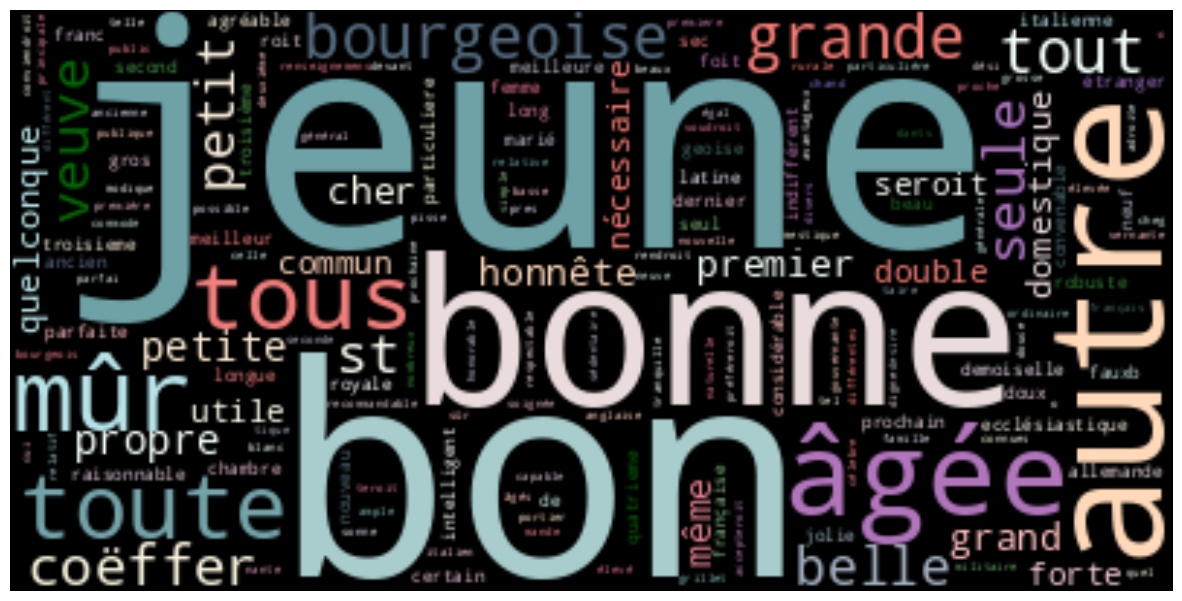
\includegraphics[width=12cm]{wordcloud_qualites_adj.png}
	\caption{Nuage de mots des adjectifs dans le corpus}
\end{figure}


Comme dans le cas des compétences, la deuxième méthode envisagée a alors consisté en l'entraînement d'un modèle de \textit{span categorization} avec spacy, toujours sur la base d'environ 500 annonces annotées, mais dont les annotations étaient cette fois dédiées aux qualités. Cette méthode s'est également révélée décevante: j'ai observé en annotant que les annonces mentionnant des qualités sont peu nombreuses (parmi les 500 que j'ai annotées, moins d'une sur dix en contient). L'entraînement du modèle a donc généré des scores de performance très faibles, voire nuls.

Face à l'échec de ces deux premières méthodes, mais maintenant forte d'une meilleure connaissance du corpus à la suite de l'annotation, j'ai donc fini par avoir recours à une méthode beaucoup plus artisanale, basée sur un mélange d'expressions régulières, de recherche de mots-clés et d'extraction d'adjectifs (à l'exception de "âgé", présent dans beaucoup d'annonces mais qui ne m'intéressent pas ici). J'ai en outre décidé de cantonner cette méthode aux dix premiers mots de chaque texte du corpus, ayant observé que les qualités que je souhaitais extraire étaient souvent placées au début de l'annonce. 

À l'aide de la fonction ci-dessous, je suis finalement parvenue à extraire des qualités pour 3096 annonces, dont on peut avoir un aperçu grâce au nuage de mot suivant. Si les adjectifs déjà présents avec la première méthode restent très visibles (jeune, bon, bonne), d'autres éléments apparaissent néanmoins: des qualificatifs physiques (jolie, agréable, ...) comme moraux ou intellectuels (recommandable, bien élevé, intelligent...). Le format du nuage de mots n'est cependant pas très utile pour restituer la présence dans le corpus d'expressions et de groupes de mots, pourtant très employés dans les annonces.

\begin{lstlisting}[language=Python,caption=Fonction destinée à extraire les qualités des annonces]
def extraire_qualites(annonce):
	qualites=[]

	# Extraire les adjectifs
	doc = nlp(annonce) 
	for token in doc:
		if token.pos_=="ADJ":
			qualites.append(token.text)
	
	qual_a_retirer=["age", "agee"]
	
	# Regex qui permet d'extraire les expressions descriptives du type "d'un beau physique", "aux moeurs honnetes"
	regex=", ?((?:d'|de |dont |au |aux )\w+'? ?\w+ (?:\w+)? (?:\w+)?),"
	qualites_regex=re.findall(regex, annonce, re.UNICODE)
	for i in qualites_regex:
		qualites.append(i)

	return " ".join(i for i in qualites if i not in qual_a_retirer)
\end{lstlisting}


\begin{figure}[ht]
	\centering
	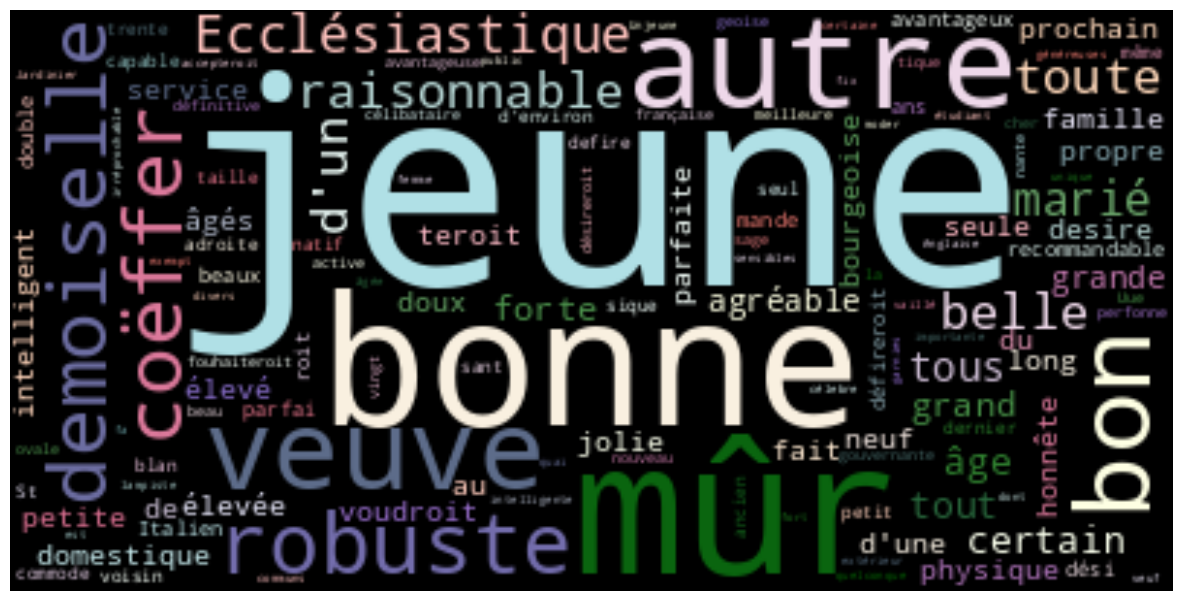
\includegraphics[width=12cm]{wordcloud_qualites.png}
	\caption{Nuage de mots des qualités dans le corpus}
\end{figure}


\section{La mise en valeur physique et intellectuelle, apanage d'une domesticité vouée à se montrer}

Un examen plus approfondi des qualités dans les annonces montre que la plupart d'entre elles se réfèrent au physique du ou de la domestique. Hormis l'adjectif "jeune", les termes les plus fréquents parmi les qualités extraites comprennent entre autres "grand" (348 occurrences), "fort" (376 occurrences), "belle" (159 occurrences), "agréable" (49 occurrences), "intelligent" (47 occurrences), "doux" (36 occurrences).

Les qualités relatives à la force et à la taille sont très majoritairement masculins: plus de trois occurrences de l'adjectif "robuste" sur quatre se trouvent dans des annonces d'hommes. Il en est de même pour l'expression "d'une belle taille" et l'adjectif "grand". La taille a une importance toute particulière dans l'embauche d'un domestique, notamment d'un valet ou d'un laquais, qui doit faire bonne figure auprès de son maître et chez qui une grande taille et une belle posture sont des indicateurs de bonne santé autant que de dignité\footcites{sabattierChapitreConditionDomestique1984}. L'intelligence figure également en bonne place parmi les qualités les plus mentionnées; encore une fois, elle est surtout masculine (65\% des annonces). 


\section{La mise en valeur morale, une qualité surtout féminine}

Un second ensemble des qualités extraites des annonces se rapporte cette fois plutôt à la moralité et à l'honnêteté des domestiques. Se présenter comme "honnête" (261 occurrences dans le corpus), ayant de "bonnes mœurs", une "bonne moralité" (254 occurrences), issue d'une bonne famille (93 occurrences) ou faisant preuve de "probité" (86 occurrences) sont autant de moyens de contrecarrer la mauvaise réputation imputée aux travailleuses et travailleurs de la domesticité. Mais ces qualités morales sont cette fois surtout l'apanage des femmes: 21\% des annonces féminines mentionnent l'honnêteté ou la probité, contre 13\% de celles des hommes. 

Aux hommes la force, aux femmes l'intégrité? Si cette distinction reproduit les attendus culturels associés aux deux sexes, la raison de sa présence parmi les annonces est peut-être plutôt à chercher du côté des conditions de travail des domestiques hommes et femmes, et donc aux préjugés et aux attendus qui leur sont associés. On l'a déjà vu, les (jeunes) hommes, qui cherchent à entrer au service d'un maître en tant que domestique particulier, une fonction qui implique de beaucoup se montrer, savent que leur physique est important sinon central, et cherchent donc à se mettre en valeur en conséquence. Les femmes, au contraire, sont chargées de tâches au sein de la maison, en ayant souvent accès au linge, à l'argenterie et à d'autres items personnels qui peuvent faire l'objet de convoitises et donc de vols de la part des domestiques. De plus, leur sexualité et leurs relations font l'objet d'une surveillance plus importante que leurs homologues masculins. On peut supposer que face à ces accusations et à cette méfiance, se présenter comme honnête (qualité renforcée ensuite par la référence à de "bons répondants") encourage voire conditionne l'embauche.


\bigskip


Les annonces d'emploi font ainsi l'objet de mises en récit et de phénomènes de publicité de soi et de son travail qui ne sont pas sans rappeler les annonces matrimoniales de la même période \footcites{jonesPersonalsPoliticsCourting2001}. La tendance est à la présentation méliorative de soi-même, de son physique comme de sa moralité, en conformité avec les normes qui entourent le travail ancillaire au XVIIIè siècle. 

Mais parfois, des  annonces sous forme de "récits de vie" semble font plutôt faire appel au registre pathétique:  "Une jeune veuve, d'un physique agréable, ayant reçu de l'éducation, appartenant à une honnête famille, ayant éprouvé de très-grands malheurs, voudroit trouver une PLACE auprès d'une personne seule pour prendre soin de son ménage, ou pour tenir un comptoir\footnote{\textit{Affiches de Paris}, 27 février 1804}"; "Une veuve âgée de 30 ans, sans suite, d'un caractère gai et doux, et d'une bonne famille, que des malheurs forcent à chercher une PLACE, desire en trouver une quelconque\footnote{\textit{Affiches de Paris}, 6 mars 1804}". Si la recherche d'emploi domestique à l'époque moderne ressemble par beaucoup d'aspects à celle d'aujourd'hui, basée sur la valorisation personnelle, d'autres éléments des annonces rappellent la dimension charitable de la domesticité au XVIIIè siècle: dans la loi comme dans les traités religieux, prendre un domestique, c'est également porter assistance aux plus démunis, en fournissant gages et logis\footcites{sabattierChapitreMaitrePere1984}. Les journaux d'annonces eux-mêmes, à leurs débuts, sont pensés comme des outils de gestion des populations indigentes, et les Bureaux d'adresses, nés du traité \textit{Sur la condition des pauvres} de Théophraste Renaudot, visent à devenir des alternatives à l'Église dans le traitement de la pauvreté. Une dimension qui transparaît également à travers l'absence presque totale de revendications (salariales ou autres) dans les annonces: dans le contexte de crise de l'emploi qui touche les grandes villes française de la seconde moitié du XVIIIè siècle, le marché de l'emploi domestique est à l'avantage des employeurs.

\chapter{Demander sans quémander: des modalités d'emploi absentes des annonces}

La mise en valeur de soi et de son travail se fait souvent aux dépends d'autres éléments dans l'annonce: les conditions matérielles d'emploi. Comment expliquer cette absence: économie de l'espace par le journal, information jugée dérisoire car tacite? 


\section{Méthode}

Les "modalités d'emploi" que je cherche à relever dans les annonces se divisent en deux ensembles. D'un côté, l'emploi ou le métier recherché; de l'autre, les conditions concrètes de travail, qui comprennent notamment les gages demandés. 

Pour ce qui est de l'emploi recherché, j'ai annoté le corpus puis entraîné un modèle de \textit{span categorization } pour reconnaître les noms de professions, de métiers et d'occupations parmi les annonces. Cette méthode a permis d'extraire une mention d'emploi dans 1506 annonces. 

Pour les gages et les conditions d'emploi plus générales, j'ai estimé que le corpus était assez homogène pour que l'analyse puisse se faire à l'aide de mots-clés. 

\section{"Cherche une place de...". Une revendication commune: l'emploi recherché}


Si l'identité professionnelle n'a pas encore sous l'Ancien Régime la valeur ni l'uniformité qu'elle prendra au XIXè puis au XXè siècle, cela n'empêche pas les domestiques en recherche d'emploi de privilégier certaines places, en raison de leur formation ou de leurs compétences. Si la majorité des domestiques travaille dans des petits foyers, où leur labeur est peu spécialisé, d'autres se trouvent au contraire insérés dans des hiérarchies ancillaires complexes, où femmes-de-chambres, valets, cochers et cuisiniers n'ont ni les mêmes tâches, ni les mêmes rémunérations, ni le même rapport à leurs maîtres. 

\begin{figure}[ht]
	\centering
	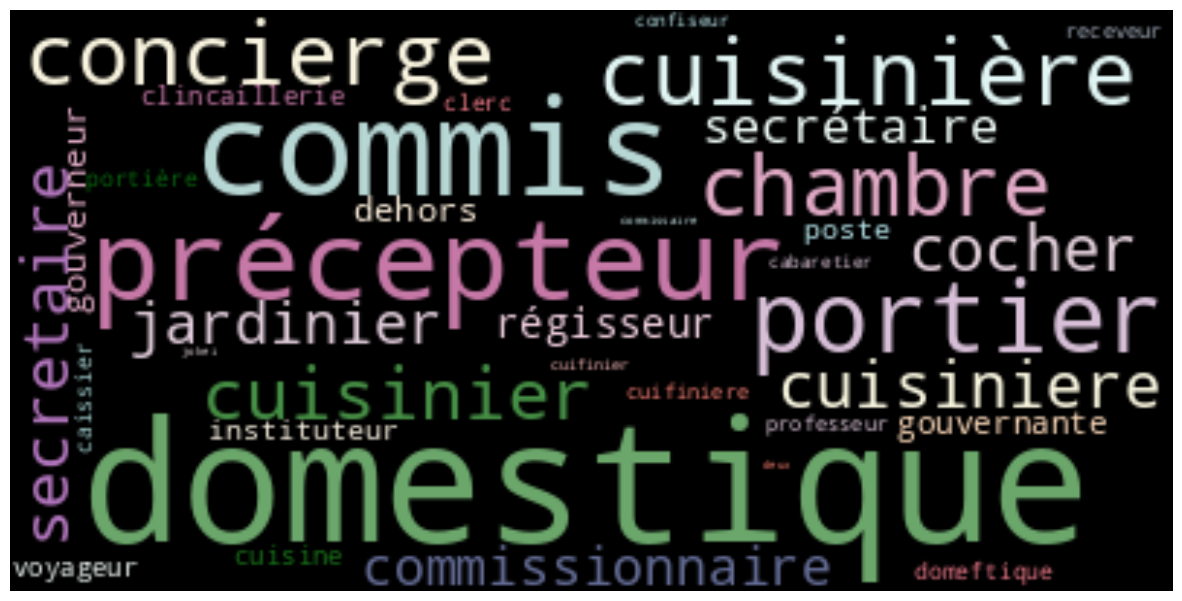
\includegraphics[width=12cm]{wordcloud_emploi.png}
	\caption{Nuage de mots des noms d'emplois dans le corpus}
\end{figure}

Les annonces reflètent cette réalité de la domesticité: si plus de deux annonces sur trois ne mentionnent pas d'emploi précis, ou alors en utilisant un qualificatif très général ("domestique"), le reste se caractérisent au contraire par la mention d'une grande diversité de rôles et de fonctions différentes: de la domesticité de confiance (secrétaire, régisseur, commissionnaire) à la domesticité chargée de l'éducation (gouvernante, gouverneur, précepteur), en passant par celle chargée d'espaces très circonscrits de la maison (jardinier, portier, cuisinier et cuisinière). 

De la même façon que les compétences ou les qualités que j'ai déjà mentionnées, les emplois sont eux aussi sexués: on observe une moins grande diversité des rôles mentionnés par les femmes, qui cherchent pour la plupart à se placer en tant que femme de chambre, cuisinière ou gouvernante, que pour les hommes, où la pluralité des conditions provient surtout des emplois domestiques plus qualifiés, souvent très spécialisés (secrétaire, instituteur, précepteur...).


\begin{table}[ht]
	\centering
	\begin{tabular}{lc}
		\hline
		\multicolumn{1}{c}{\textbf{Emploi}} & \textbf{Occurrences} \\ \hline
		domestique                          & 315                  \\
		commis                              & 153                  \\
		précepteur                          & 128                  \\
		cuisinière                          & 124                  \\
		valet                               & 86                   \\
		femme de chambre                    & 69                   \\
		portier                             & 68                   \\
		secrétaire                          & 51                   \\
		concierge                           & 45                   \\
		cuisinier                           & 45                   \\
		jardinier                           & 33                   \\
		cocher                              & 25                   \\
		commissionnaire                     & 22                   \\
		régisseur                           & 13                   \\
		gouvernante                         & 13                   \\
		gouverneur                          & 12                  \\ \hline
	\end{tabular}
	\caption{Emplois les plus fréquents dans le corpus (plus de dix occurrences)}
\end{table}


\begin{figure}[ht]
	\centering
	\begin{subfigure}[b]{0.4\textwidth}
		\centering
		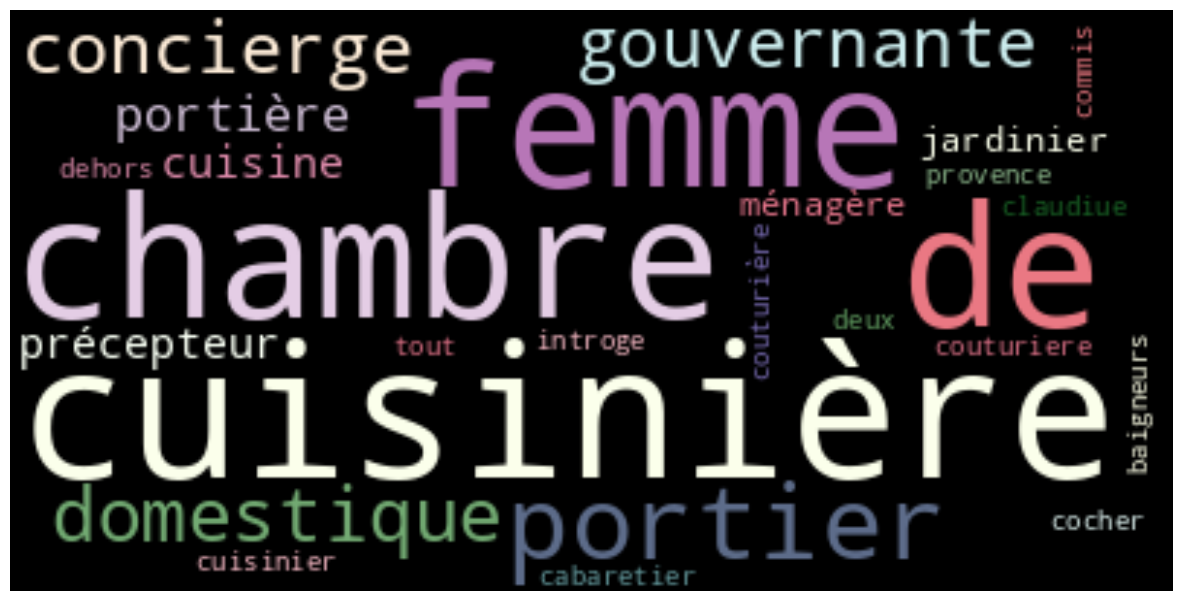
\includegraphics[width=6cm]{wordcloud_emploi_F.png}
	\end{subfigure}
	\begin{subfigure}[b]{0.4\textwidth}
		\centering
		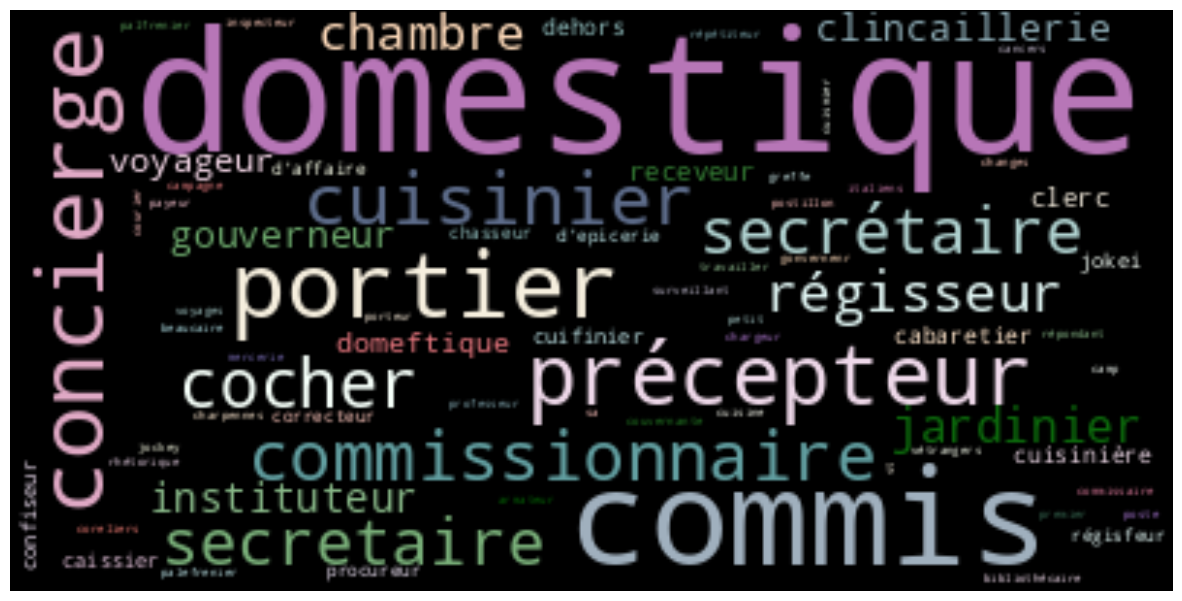
\includegraphics[width=6cm]{wordcloud_emploi_H.png}
	\end{subfigure}
	\caption{Nuage de mots des compétences dans les annonces écrites par des femmes (gauche) et par des hommes (droite)}
\end{figure}


Enfin, l'étude des \textit{Affiches} est également l'occasion d'observer l'apparition d'activités moins communes, concomittantes de certaines transformations de l'espace urbain, comme dans cette annonce parisienne en date du 18 mars 1804: "Un homme et sa femme, sans enfans, ayant travaillé dans les bains les plus en réputations de Paris, possédant toutes les connaissances requises pour ce genre de travail, entr'autres celle des bains épilatoires des douches et de vapeur et de propretés en se baignans ou sans se baigner, desirent se PLACER comme baigneurs, soit à Paris ou dans les départemens; à Paris ils leur seroit indifférent de se placer séparément. S'adresser par écrit, au portier de ce Journal\footnote{\textit{Affiches de Paris}, 18 mars 1804}."


\section{L'omission des gages et des conditions de travail : stratégie ou nécessité? }

Face à cette présence minoritaire mais régulière des noms de métiers et des spécialisations domestiques dans les annonces, l'absence de revendications de rémunérations ou de conditions de travail apparaît encore plus flagrante.

Gages et appointements sont presque inexistants dans le corpus. Seules 48 annonces mentionnent d'une façon ou d'une autre une rémunération: parmi elles, 41 disent "se contenter d'un appointement modique" (parfois limité à la table ou au logis) voire ne pas exiger de gages du tout (parfois pour une période donnée, parfois avec des justifications assez absurdes: "quoi-que ses talents méritent des appointements, il n'en exigera point\footnote{\textit{Affiche de Lyon}, 11 juin 1772.}", parfois en précisant avoir un autre revenu, le plus souvent une rente), trois ont des revendications précises, parfois liées à des qualifications ou des spécialisations domestiques ("pas moins de 200 francs\footnote{\textit{Affiches de Paris}, 19 mars 1804.}", "ne se déplacera pas qu'on ne lui donne un avantage et cent écus ou au moins deux cents cinquantes livres de gages par an\footnote{\textit{Affiches de Lyon}, 30 août 1769.}", "deux à trois cents livres d'appointement par an\footnote{\textit{Affiches de Lyon}, 14 octobre 1767.}"), et quatre sont des offres d'emploi.
 
En dehors des gages, les seules revendications de la part des domestiques consistent généralement à demander à se placer "dans quelque bonne maison" (255 annonces), ou auprès de personnes spécifiques: femmes ou hommes seuls, ou au contraire dans des maisons avec de jeunes enfants. Les demandes liées à une envie de voyager (252 annonces) ou de vivre à la campagne sont également relativement nombreuses, et témoignent de l'espace de liberté et d'ouverture des possibles que représente le journal de petites annonces, ainsi que l'a déjà signalé Ulrike Krampl\footcites{kramplAdresserClercHuissier2017}. 

Sans comparaison avec d'autres périodicités, il est difficile de dire si cette absence des conditions de travail est commune dans les annonces, les gages étant discutés de vive voix, ou si elle résulte d'un contexte économique difficile pour les domestiques, qui se voient obligés d'accepter les gages et les circonstances proposées par les employeurs. 


	\part{De l'annonce à l'emploi:  rôle et place des répondants, des intermédiaires et de l'adresse dans les \textit{Affiches}}


\chapter{Répondants et certificat: l'importance de la cooptation et des réseaux d’information}

Une partie essentielle des annonces, peut-être la plus importante aux yeux des domestiques qui les écrivent, a pour l'instant échappé à l'analyse: il s'agit de l'adresse, toujours placée en fin d'annonce, et dont l'étude révèle beaucoup au sujet des liens et des processus sociaux à l'œuvre dans la recherche d'emploi au XVIIIè siècle. 

Mais avant même de mentionner une adresse ou un intermédiaire, les annonces mettent en avant des références, des individus susceptibles d'informer un potentiel employeur des qualités et de l'honnêteté du ou de la domestique. Complémentaire de la mise en valeur de sa propre personne ou de son labeur, la mention des "bons répondants" fait écho à l’importance des réseaux informels dans la recherche de travail au XVIIIè siècle. Garants à la fois de sérieux et de bonnes mœurs, les répondants ne concernent pas seulement le travail domestique: ils sont également nécessaires dans certaines manufactures, pour rejoindre un atelier ou une communauté de métier\footcites[p.86-87]{crowstonFabricatingWomenSeamstresses2001}, et même dans les ateliers de filature mis en place sous la Révolution pour fournir du travail aux plus démunies\footcites[p.43]{dicaprioOriginsWelfareState2007}. Mais la référence dans la domesticité, où travailleurs et travailleuses sont soumis à une méfiance de tout instant parce qu'ils pénètrent l'espace privé du maître et se voient accorder sa confiance, est primordiale. Dans la seconde moitié du XVIIIè siècle, où la défiance de la noblesse et de la bourgeoisie envers les classes laborieuses croît encore, elle devient indispensable. Elle se double même d'un mode de référencement institutionnel, avec l'apparition du certificat dès le XVIè siècle\footcites{guttonDomestiquesServiteursDans1981}, dans lequel les domestiques ont obligation de consigner le contact de leurs anciens employeurs, voire d'obtenir leur accord écrit avant de prendre congé. Loin d'être répandu, le certificat représente néanmoins un moyen fort de régulation du travail ancillaire, notamment aux yeux de la police urbaine. 

Dans le cas des petites annonces, ces répondants et leur rôle de "médiatisation de la confiance\footcites{kramplAdresserClercHuissier2017} sont d'autant plus importants qu'on s'éloigne des réseaux traditionnels de l'embauche que sont le voisinage, l'interconnaissance, la clientèle, la recommandation par un domestique déjà dans la maison ou par un proche. Ainsi, loin de subvertir ou de supplanter les logiques et procédures instituées de l'Ancien régime et favorables aux maîtres, le nouveau support que représente l'annonce semble à première vue plutôt s'y conformer.



\section{Méthode}

Ayant pu observer que les formes de recommandations contenues dans les annonces sont très régulières et adoptent des formules qui varient peu dans le temps ou selon la ville, j'ai eu recours pour les extraire à des expressions régulières. J'ai d'abord noté que le mot privilégié dans les annonces est "répondant", le plus souvent employé dans la formule "[Le domestique] fournira de bons répondants". Il a ensuite fallu prendre en compte les possibles variations typographiques ou erreurs d'océrisation ("e" accentué ou non, présence d'un "t" ou non à la fin du mot), ainsi que les possibles coupures du mot en fin de ligne. J'ai ensuite pu ajouter une colonne à mon \textit{dataframe}, précisant cette fois simplement si l'annonce contient ou non l'expression régulière.

Afin de m'intéresser aux possibles qualificatifs appliqués aux répondants, j'ai en outre extrait, à partir des textes des annonces, les bigrammes et trigrammes qui contiennent le mot répondant, que j'ai également ajoutés au \textit{dataframe}.

Pour ce qui est du certificat, j'ai employé la même méthode, à partir de l'expression \fbox{cer-?ti-?fi-?ca}.


\section{"De bons répondants": une mention essentielle des annonces}

L'expression ainsi élaborée, \fbox{re?é?-?pon-?dan}, m'a finalement permis de constater que plus d'une annonce sur cinq contiennent une référence aux répondants (1151 sur 5064). Parmi elles, plus des trois quarts (930 annonces) précisent avoir de "bons" ou "les meilleurs" répondants. 

Par ailleurs, la mention des répondants semble assez peu impactée par la variable de genre: un peu moins d'un tiers des annonces déposées par des femmes sont concernées, contre un quart pour les hommes. Étant donné les limites de la catégorisation sexuée dans le corpus, et le fait que la majorité des annonces n'ont pu être classées, je considère que cette différence est assez négligeable. 


\begin{figure}[h]
	\centering
	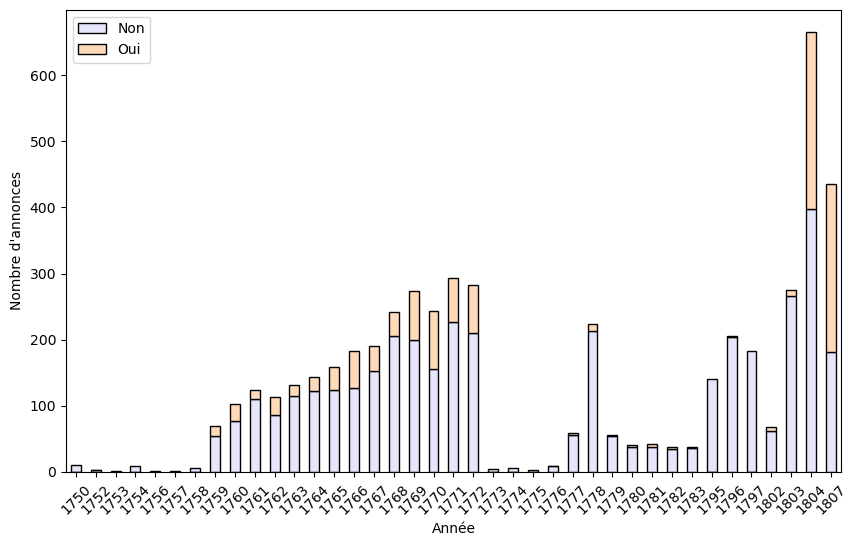
\includegraphics[width=12cm]{hist_rep_chrono.png}
	\caption{Répartition de la mention des répondants selon le temps}
\end{figure}

Enfin, la présence ou non des répondants dans l'annonce évolue au cours du temps: si les annonces "avec répondants" réprésentent entre un dixième et un quart des annonces dans les années 1760 et 1770, elles sont plus d'un tiers en 1804, et plus de la moitié en 1807. 

En comparaison, la présence du certificat dans les annonces est beaucoup plus rare, et finalement proportionnel à son impact réel sur le monde de la domesticité: seules 199 annonces le mentionnent.


\chapter{"S'adresser à ...". Intermédiation, modes d'adressage et capacités d'agir des domestiques}

Si l'omniprésence des références et des répondants dans les annonces est un indicateur du maintien et de la persistance de logiques de cooptation et de recherche d'emploi spécifiques à l'Ancien Régime, le journal d'annonces ne peut pas être analysé uniquement comme un moyen parmi d'autres de trouver un travail. En proposant un nouveau support, les \textit{Affiches} proposent également de potentielles nouvelles stratégies et manœuvres à disposition des domestiques: "la petite annonce pose ainsi la question de l’articulation entre ce nouveau support et la problématique exigence d’un "travail de confiance" inhérent aux relations laborieuses\footcites{kramplAdresserClercHuissier2017}". 


\section{Méthode}

L'adresse est probablement la partie la plus uniforme et la plus stable dans le temps de l'annonce. C'est cette régularité qui m'a permis de l'inclure parmi les catégories de \textit{spans} à extraire avec le modèle entraîné sur Spacy; de la même façon qu'avec les compétences ou les emplois, un peu plus de 500 annonces ont été annotées en vue de l'entraînement.  

Au final, ce sont 1184 annonces pour lesquelles le modèle a permis d'extraire une adresse. 


\section{Intermédiaires et adresses: aperçu du réseau urbain de l'information}

L'extraction de l'adresse des annonces aurait pu donner lieu à une tentative d'esquisse de la géographie domestique à l'aide de techniques de spatialisation de l'information. Ayant manqué de temps pour mener à bien ce projet dans le cadre de ce mémoire, je présente ici quelques pistes de réflexion autour des modes d'adressage et des intermédiaires des petites annonces, largement inspirées de l'article qu'Ulrike Krampl a dédié à la question\footcites{kramplAdresserClercHuissier2017}. 

Tout d'abord, le mode d'adressage signalé au sein des annonces est en très grande partie implicite; "s'adresser à" signifie conventionnellement s'adresser à l'oral, en personne, si bien que seules onze annonces du corpus précisent "s'adresser verbalement" ou "de vive voix". Certaines indiquent néanmoins les heures auxquelles on peut les trouver chez eux:  "S'ad. verbalement, le matin jusqu'à 2 heures, chez Madame S. D., rue St.-An-toine, n. 58, maison de l'épicier, en face du théâtre Mareux\footnote{\textit{Affiches de Paris}, 13 mars 1807}". 63 annonces, en revanche, précisent qu'il faut répondre à l'annonce par écrit ou par lettres, et le plus souvent franc de port. 

Dans son article, Ulrike Krampl remarque que trois types d'adresses peuvent être indiquées par les domestiques: "celle du bureau, celle des particulier.es concerné.es et celle d’intermédiaires". Dans ce corpus, les annonces qui renvoient à un bureau d'adresses (du journal ou autre) sont très minoritaires: je n'ai pu en retrouver que 109, toutes parues dans les années 1760 à Lyon ou entre 1804 et 1807 à Paris. La pratique majoritaire semble donc être le renvoi vers son adresse particulière ou l'adresse d'un ou d'une intermédiaire, la différence entre les deux étant d'ailleurs difficilement perceptible dans les annonces.

En outre, Ulrike Krampl s'intéresse dans son article à la sociologie du groupe des intermédiaires. Elle remarque que ceux-ci sont en grande partie voire en majorité des officiers publics, hommes de droit ou de l'administration dont le rôle de médiation entre individus est déjà attesté dans d'autres sphères que la presse, et qui répondent au besoin de contrôle et d'institutionnalisation des \textit{Affiches}. Néanmoins, cette configuration marquée par un processus de "judiciarisation" des annonces ne semble pas se retrouver dans ce corpus: parmi les métiers du droit et de la justice signalés par l'historienne (procureur, huissier, clerc et commis, ...), je ne retrouve que les notaires, qui demeurent très rares avec 12 occurrences, et un unique avocat. En revanche, d'autres professions, signalées par U. Krampl mais définies comme marginales, se retrouvent beaucoup plus dans mon corpus: les portiers notamment, dont l'historienne ne retrouve que quatre occurrences (3,4\% de son corpus, et uniquement dans des offres d'emploi), sont ici au moins au nombre de 87, soit plus de 7\%. Les marchands quant à eux, se retrouvent dans des proportions assez similaires entre les deux corpus: ils sont les intermédiaires de 6,7\% des annonces chez Ulrike Krampl et de 5,2\% des annonces ici.

Enfin, l'étude du genre des intermédiaires corrobore également les observations générales de l'article: l'intermédiation est majoritairement une activité d'hommes, mais où les femmes peuvent se faire une place. Elles sont même un peu plus présentes dans mon corpus, passant de 9,4\% des intermédiaires chez Ulrike Krampl à près de 30\% des annonces qu'il m'a été possible de genrer (197 femmes sur 667 annonces). 


\section{“On ne recevra pas de lettres des petits bureaux”: l'annonce comme alternative au marché traditionnel du travail?}

Parmi les annonces et les formules d'adressage, une phrase revient dans plusieurs dizaines d'annonces: "On ne recevra pas les lettres des petits bureaux". Cette formule fait référence aux bureaux de placement, un nouveau mode d'intermédiation et de recherche de travail, qui apparaît au XVIè siècle, comme l'annonce, dont il est l'un des premiers émetteurs. Les bureaux ont la particularité au XVIIIè siècle de tenir des registres de domestiques, qui se veulent autant des outils de centralisation de l'information que de régulation et de contrôle de l'activité ancillaire: à partir des témoignages de leurs anciens maîtres, ils indiquent les bonnes et mauvaises qualités des domestiques, les maisons qu'ils ont servies et tout renseignement qui pourrait intéresser un potentiel employeur, lequel a parfois d'ailleurs droit à une "période d'essai" avec le valet ou le serviteur recommandé par le bureau\footcites{sabattierChapitreConditionDomestique1984}. 

Si, dans les faits, les bureaux de placement ont un impact très limité par rapport à l'importance des réseaux informels de cooptation et d'intermédiation au XVIIIè siècle (ils sont au nombre de deux ou trois à Paris à la fin du siècle), ils semblent faire l'objet de nombreux reproches de la part des domestiques en recherche d'emploi, peut-être du fait de leurs techniques commerciales agressives ou de leur taux de succès limité, en témoigne cette annonce publiée à Paris en mars 1804: "Un citoyen d'un âge mûr, sachant raser, coëffer, faire une petite cuisine en cas de besoin, le service de la chambre et de la table, panser let chevaux, mener un cabriolet, desire se PLACER à Paris ou à la campagne. Il est muni de bons certi-ficats et a de bons répondans. S'adres. à Mad. Roytel, mar-chande limonadiere, rue Joubert, n. 515, Chaussée d'Antin, pour remettre au cit. Baptiste. On ne recevra pas de lettres des petits bureaux qui prétendent donner des places\footnote{\textit{Affiches de Paris}, 30 mars 1804}"
Ces références aux bureaux de placement restent marginales dans le corpus d'annonces, mais elles donnent certains indices sur la façon dont les individus naviguent au milieu des différents supports et réseaux qui sont à leur disposition pour trouver du travail, et qui se multiplient à l'ère de la presse de grand tirage. L'anonymat permis par l'annonce, notamment, représente un changement important par rapport aux siècles précédents. Les précisions apportées par certains demandeurs, qui souhaitent qu'on s'adresse à tel commerce ou telle maison "sans (...) dire le sujet\footnote{\textit{Affiches de Paris}, 30 mars 1804}" de sa demande ou sans "faire aucune question au portier\footnote{\textit{Affiches de Paris}, 19 mars 1804}", permettent d'envisager les journaux d'annonces comme permettant une marge de manoeuvre vis-à-vis des réseaux traditionnels du travail domestique, notamment lorsqu'on souhaite trouver un nouvel emploi sans en informer ses maîtres ou ses proches. Une perspective déjà évoquée par Clyde Plumauzille et Ulrike Krampl\footcites{kramplPresseAnnoncesParisienne2020}: l'annonce devient alors "un outil émancipatoire par rapport aux logiques de contrôle inhérentes à l’interconnaissance, à la recommandation et au bureau de placement". 

\bigskip

Ainsi, si les demandes d'emploi dans la presse montrent de nombreux signes de la persistance de logiques de cooptation spécifiques à l'Ancien régime (en premier lieu, l'importance des référents et des garants), elles donnent également des indices sur les façons dont les individus se saisissent de supports inédits pour former des stratégies face à un marché qui leur est défavorable, et où peut parfois s'exprimer une capacité d'agir nouvelle.

	\part{Envisager la division sociale et sexuée du travail à partir des annonces: l'apport du \textit{topic modeling}}


\chapter{L'échec du LDA (\textit{Latent Dirichlet Allocation})}


Le \textit{topic modeling} est une méthode d'apprentissage non-supervisé qui emploie un modèle de probabilité pour associer des textes ou des parties de textes à des thèmes, ou \textit{topics}. Dans les faits, le \textit{topic model} va effectuer une opération de \textit{clustering}, c'est-à-dire tenter de rapprocher certains mots du corpus entre eux, en se basant sur leur similarité sémantique supposée. 

Appliqué au corpus de petites annonces, le \textit{topic modeling} peut être un moyen d'étoffer et de proposer un regard complémentaire et englobant aux incursions très localisées qui ont été faites jusqu'ici. 

\section{Méthode}


Le premier algorithme de \textit{topic modeling} que j'ai essayé d'appliquer au corpus est le LDA, ou \textit{Latent Dirichlet Allocation}, via la librairie python Gensim\footnote{Le site et la documentation de la librairie: \url{https://radimrehurek.com/gensim/}}. Le LDA est un modèle statistique qui repose sur l'hypothèse que chaque mot du corpus peut être associé à un \textit{topic}, en se basant sur la co-occurrence des mots au sein du corpus, considéré comme un sac de mots.

Le LDA s'applique donc sur un texte lemmatisé et sans stopwords, puisqu'il considère que chaque mot du corpus peut être associé à un \textit{topic} et possède donc une valeur sémantique définie. L'une des grandes différences entre le LDA et d'autres méthodes de \textit{topic modeling} est que les modèles de LDA nécessitent qu'on leur précise le nombre de \textit{topics} à générer. Dans le cas des annonces, j'ai ainsi pu tester l'algorithme de gensim et comparer les scores de performance du modèle en fonction du nombre de \textit{topics} générés. 

 

\section{Des résultats peu significatifs pour notre corpus}

Gensim génère deux scores de performance différents: la perplexité du modèle d'un côté, et sa cohérence de l'autre. La perplexité est une mesure de la surprise du modèle face à des données inédites, qu'il n'a jamais vues. En d'autres termes, une mesure d'à quel point de nouvelles données sont probables ou attendues étant donné les données que le modèle a déjà ingérées. Plus ce score est bas, moins le modèle a de chances d'être "surpris", et donc meilleur il est. Cependant, la perplexité en tant que score de performance a des limites, la première étant qu'elle est souvent décorrélée du jugement humain sur ce qui constitue un \textit{topic} pertinent ou non; en d'autres termes, elle n'est pas facilement interprétable\footcites{changReadingTeaLeaves2009}.  La cohérence du modèle, quant à elle, représente la similarité sémantique entre les mots au sein d'un \textit{topic}; elle est donc plus utile pour estimer l'efficacité réelle d'un modèle. On considère qu'un bon score de cohérence est compris entre 0.5 et 0.7. 

\begin{table}[ht]
	\centering
	\begin{tabular}{ccc}
		\hline
		\textbf{Topics} & \textbf{Cohérence} & \textbf{Perplexité} \\ \hline
		10                        & 0.37                        & -7.94                        \\
		20                        & 0.4                         & -15.01                       \\
		30                        & 0.39                        & -18.88                       \\
		40                        & 0.41                        & -22.73                       \\
		50                        & 0.4                         & -26.59                       \\
		60                        & 0.4                         & -30.59                       \\
		70                        & 0.39                        & -34.45                       \\
		80                        & 0.39                        & -38.41                       \\
		90                        & 0.39                        & -42.28                       \\ 
		100                       & 0.38                        & -46.28                       \\ \hline
	\end{tabular}
	\caption{Scores de performance du modèle en fonction du nombre de topics générés}
\end{table}

Néanmoins, avec un corpus nettoyé au préalable, on observe que la cohérence du modèle appliqué aux petites annonces ne dépasse jamais 0.41. L'examen des 40 thèmes générés par ce modèle met en évidence les difficultés du LDA sur ce corpus: les cinq premiers \textit{topics} contiennent des mots très rares dans le corpus, dont certains ont même plutôt l'air de résulter d'erreurs d'océrisation ou de segmentation des annonces. Les \textit{topics} suivants sont déjà plus cohérents (topic 7 sur les compétences féminines et manuelles, topic 8 sur les éléments de langage qui caractérisent l'annonce: placer, adresser, écrire, demande...) mais peuvent aussi présenter des redondances.

Ainsi, l'emploi du LDA et de gensim ne s'est pas révélé probant pour ce corpus. Plusieurs raisons pourraient expliquer cela: la longueur limitée des documents (bien qu'une découpe tous les 500 mots n'ait pas donnée de meilleurs scores qu'une découpe par annonce), la présence d'\textit{outliers} et d'anomalies qui rendent difficile une généralisation du modèle. 

\begin{figure}[ht]
	\centering
	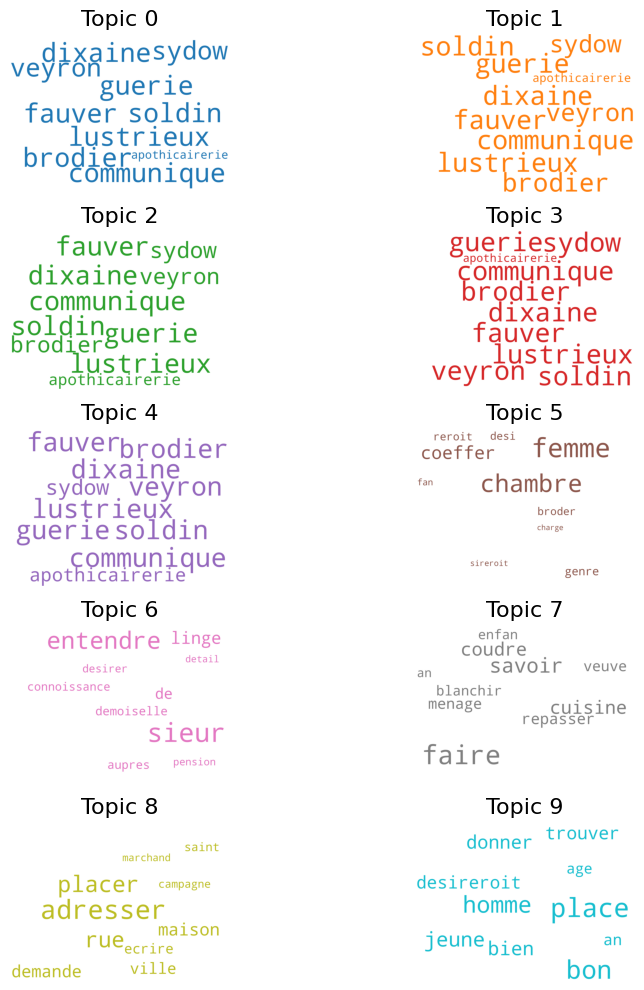
\includegraphics[width=12cm]{wordcloud_LDA.png}
	\caption{Nuage de mots des dix premiers topics du modèle}
\end{figure}




\chapter{Cartographier les frontières du travail et des annonces avec Top2Vec}

\section{Méthode}

Un second ensemble de \textit{topic models} repose cette fois non pas sur la co-occurrence de mots mais sur des \textit{embeddings}, c'est-à-dire une représentation vectorisée des mots du corpus et de leurs relations sémantiques. La première librairie que j'ai utilisée est Top2Vec, dont le fonctionnement est décrit de la manière suivante par ses créateurs: "L'algorithme postule que des documents similaires sémantiquement sont indicateurs d'un topic sous-jacent. La première étape est de créer un \textit{embeddin}g de document et de vecteurs de mots. Une fois les documents et les mots représentés dans un espace vectoriel, le but de l'algorithme est de trouver les amas les plus denses de documents, puis d'identifier quels mots ont attiré ces documents les uns vers les autres. Chaque amas est un topic, et les mots qui ont attiré les documents vers cet amas sont les mots appartenant au topic.\footnote{Description disponible sur le github de Top2Vec: \url{https://github.com/ddangelov/Top2Vec}}".
Ainsi, à l'inverse de Gensim, Top2Vec ne nécessite pas qu'on lui fournisse un nombre de\textit{ topics} prédéfinis, ni qu'on lemmatise ou nettoie de quelconque façon le corpus avant de le donner au modèle. L'un des seuls paramètres qu'on peut lui fournir au moment de la génération des \textit{embeddings} puis des \textit{topics} est la vitesse d'apprentissage (j'ai ici utilisé l'option "deep-learn", la plus lente mais qui fournit en théorie des résultats plus cohérents). Néanmoins, une fois les \textit{topics} générés, de nombreux traitements sont possibles.

Top2Vec appliqué au corpus des \textit{Affiches} génère 24 topics, que pour beaucoup on peut interpréter comme révélant un aspect ou une dimension des petites annonces d'emploi, qu'elle soit relative à l'économie de l'annonce, à la division et à la description du travail, voire même aux limites intrinsèques au corpus. 


\section{Économie de l'annonce}

Tout d'abord, plusieurs \textit{topics} générés par Top2Vec ont pour objet des éléments distinctifs des petites annonces, notamment les phénomènes d'adressage et d'intermédiation, visibles dans les topics 14 et 20 avec des mots comme "recevra", "ad(resser)", "lettres", "renseignemens". Les marques de la mise en valeur de soi sont également rendues visibles par le topic 21, qui met en avant les valeurs centrales que représentent l'honnêteté et la fidélité dans l'\textit{ethos} domestique.

\begin{figure}[ht]
	\centering
	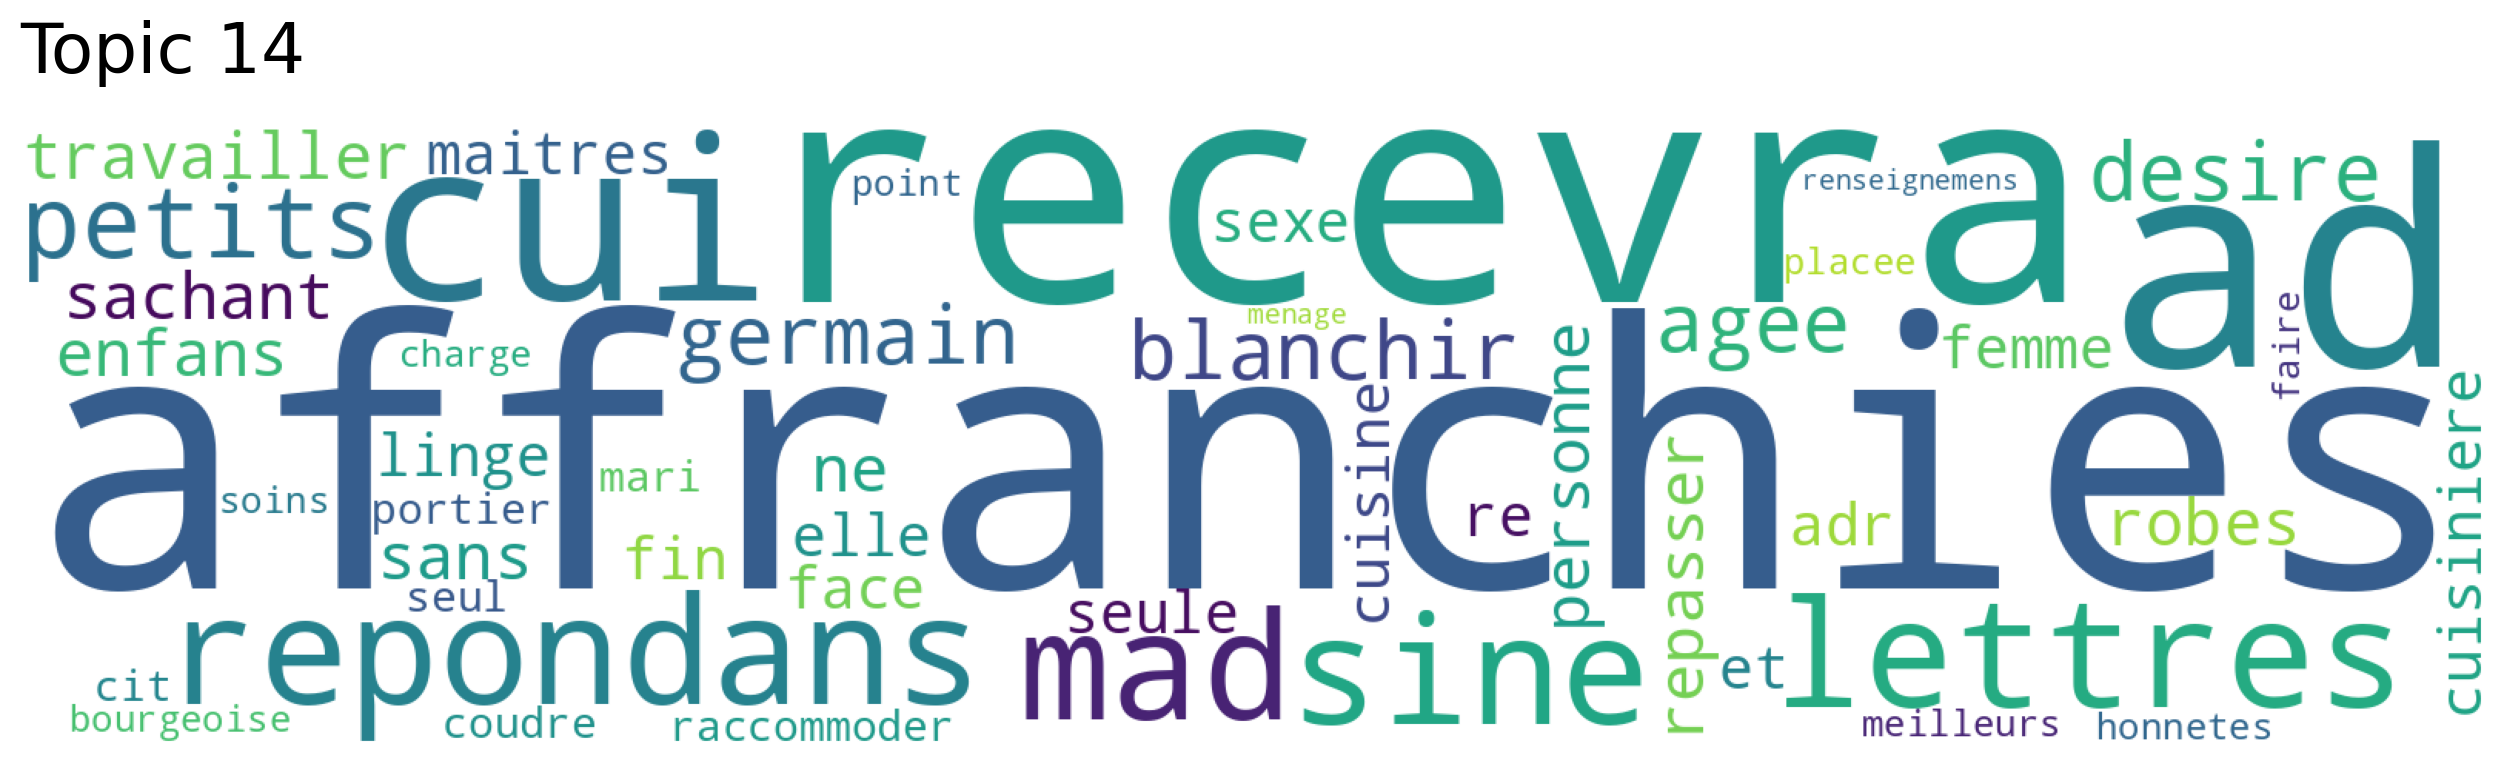
\includegraphics[width=12cm]{wordcloud_top2vec_14.png}
	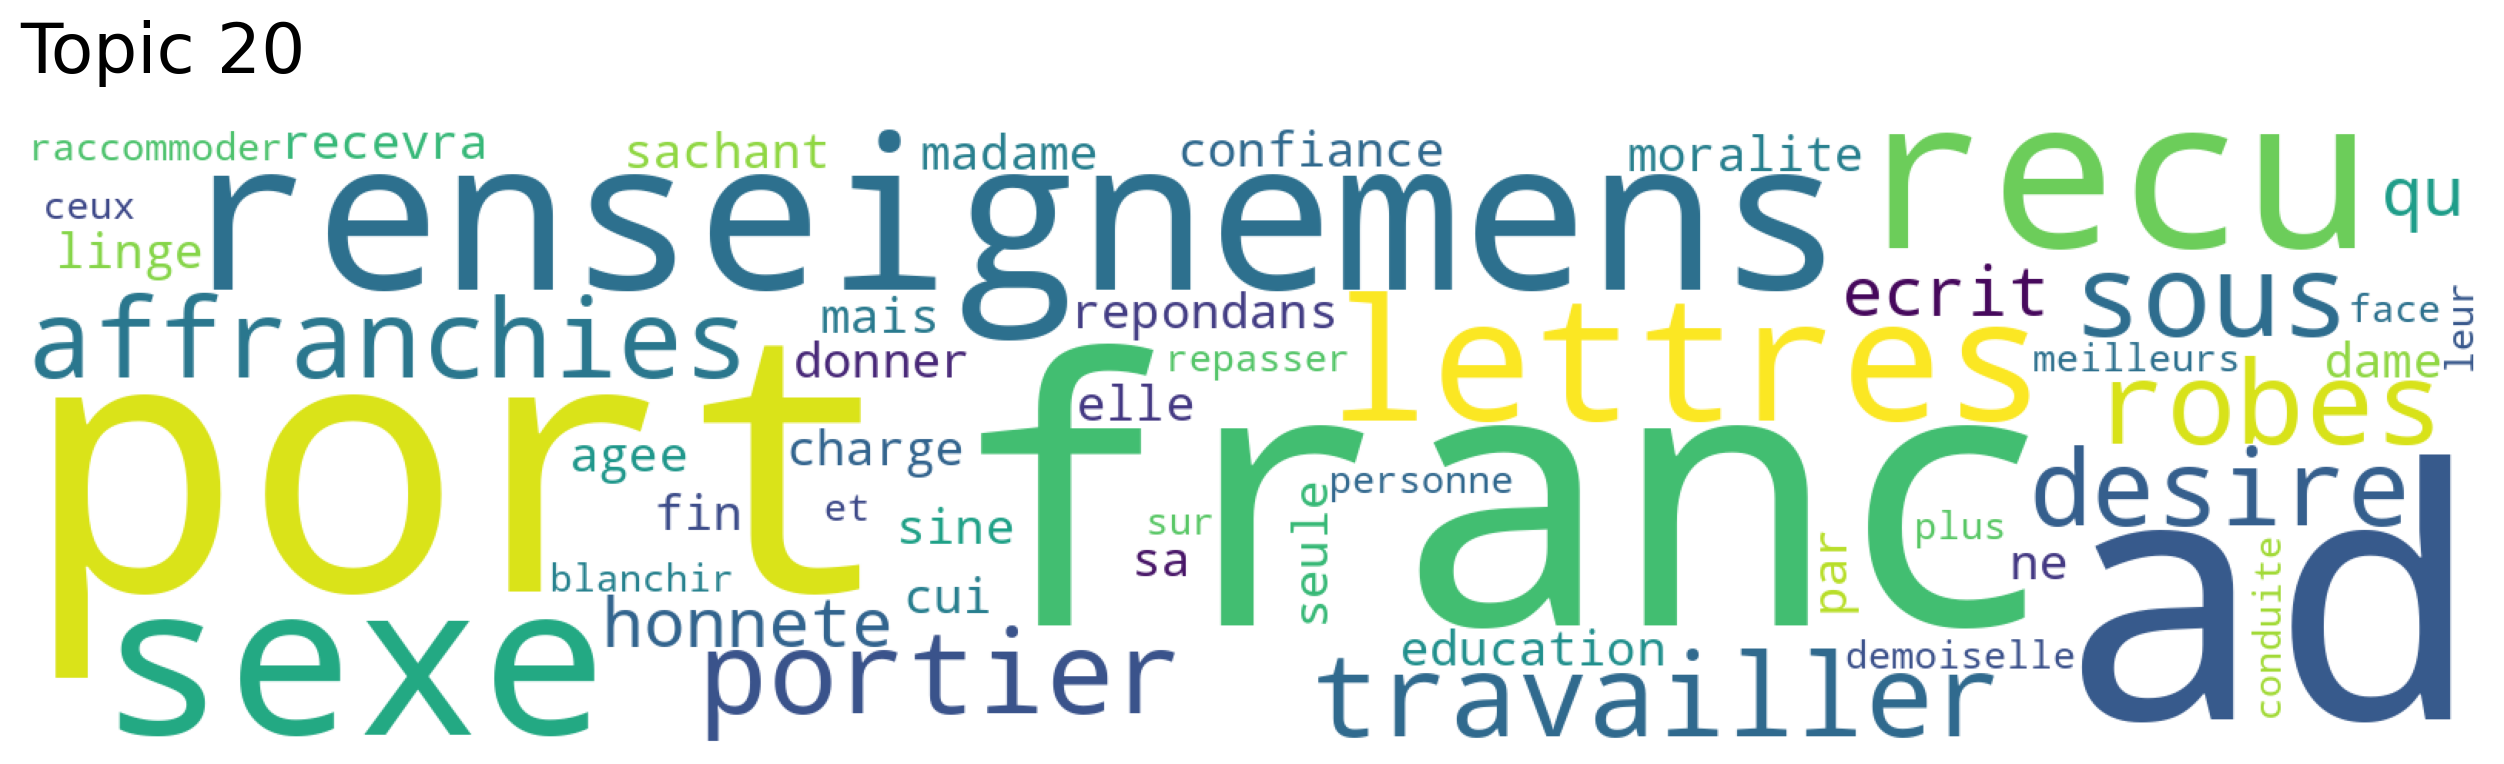
\includegraphics[width=12cm]{wordcloud_top2vec_20.png}
	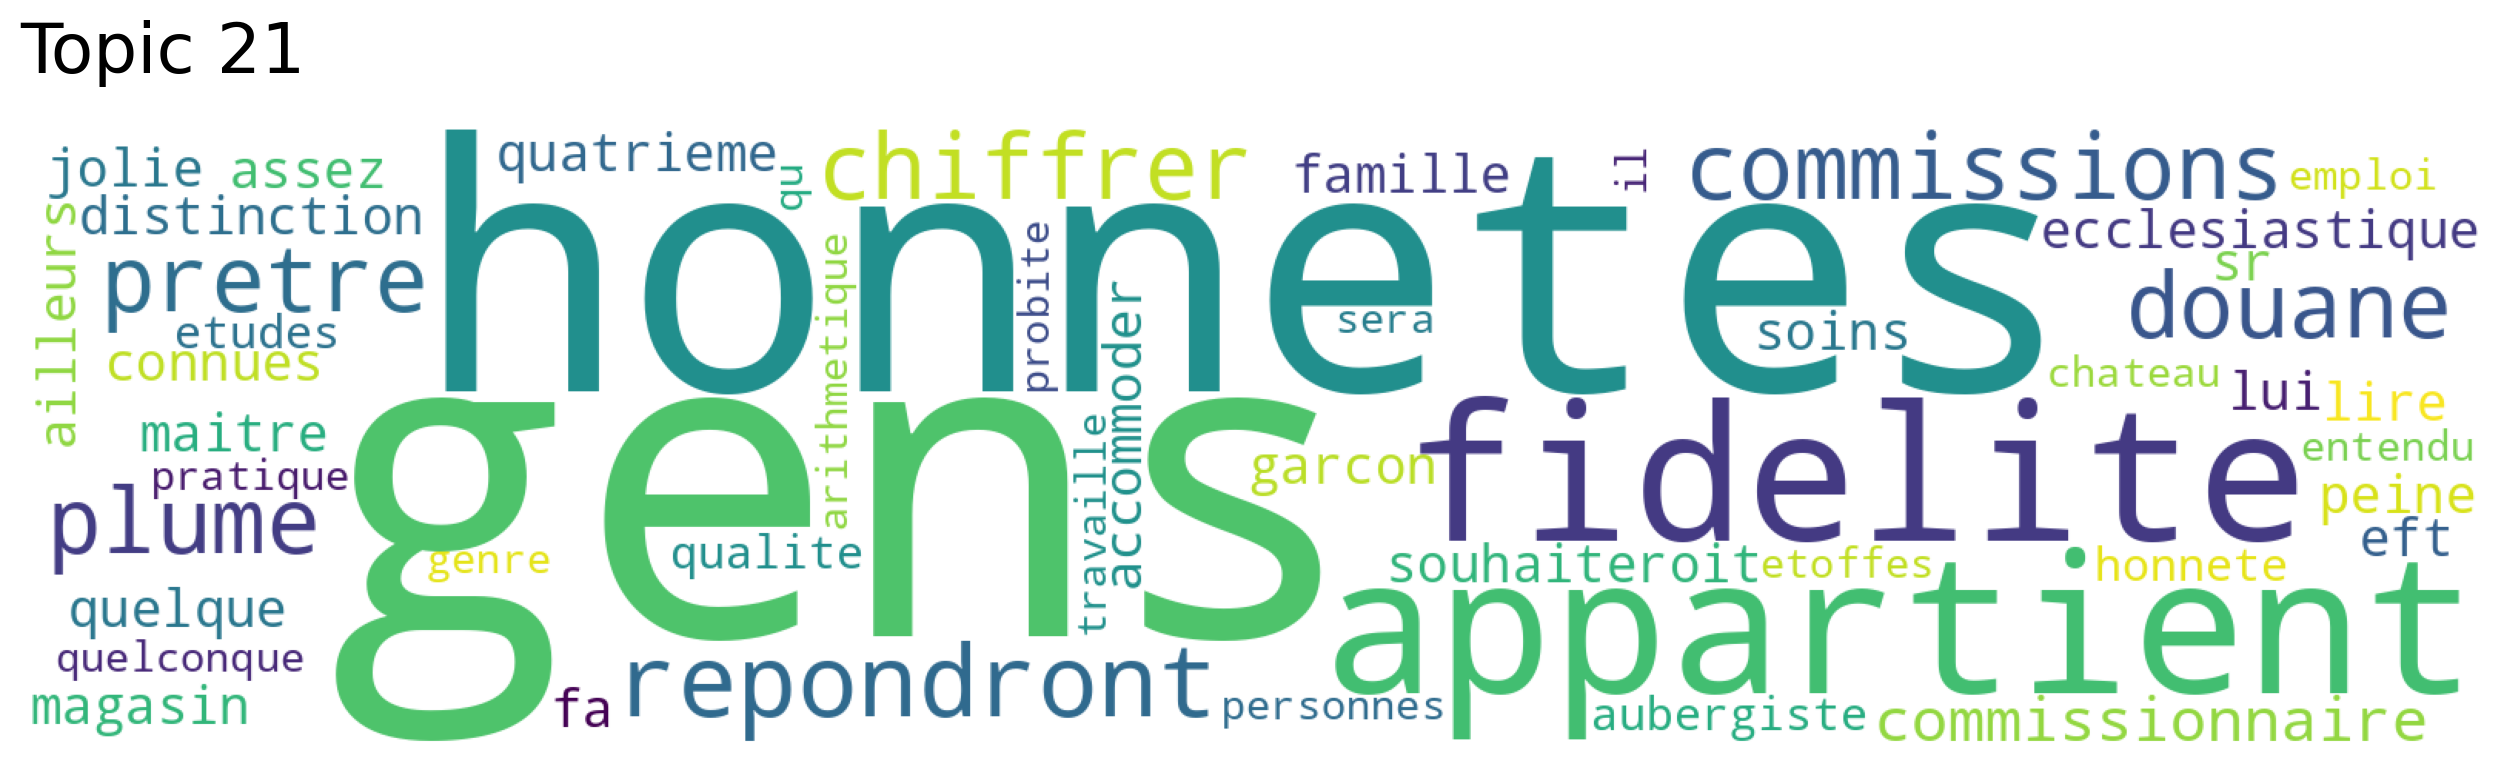
\includegraphics[width=12cm]{wordcloud_top2vec_21.png}
	\caption{Nuage de mots des topics 14, 20 et 21}
\end{figure}

\section{Des \textit{topics} genrés...}

Une deuxième observation qui peut être faite, et qui corrobore ce qu'on a déjà vu au chapitre 7, est celle d'une division fortement sexuée du travail domestique, rendue manifeste à travers la distinction par l'algorithme des compétences selon le sexe. D'un côté, les topics 0, 1 et 3 (qui comptent par ailleurs parmi les topics les plus importants du modèle) se rapportent plutôt aux travaux féminins, que ce soit à travers des qualificatifs de genre (fille, dame, veuve, citoyenne), des qualificatifs d'emplois ou de places (gouvernante) ou des verbes de compétences (raccommoder, cuisiner, blanchir, repasser). À l'inverse, les topics 2, 9 et 12 se rapportent plutôt à la domesticité masculine, encore une fois à travers des noms (garçon), des adjectifs (robuste) et des verbes (raser, panser, conduire, coiffer). 


\begin{figure}[h!t]
	\centering
	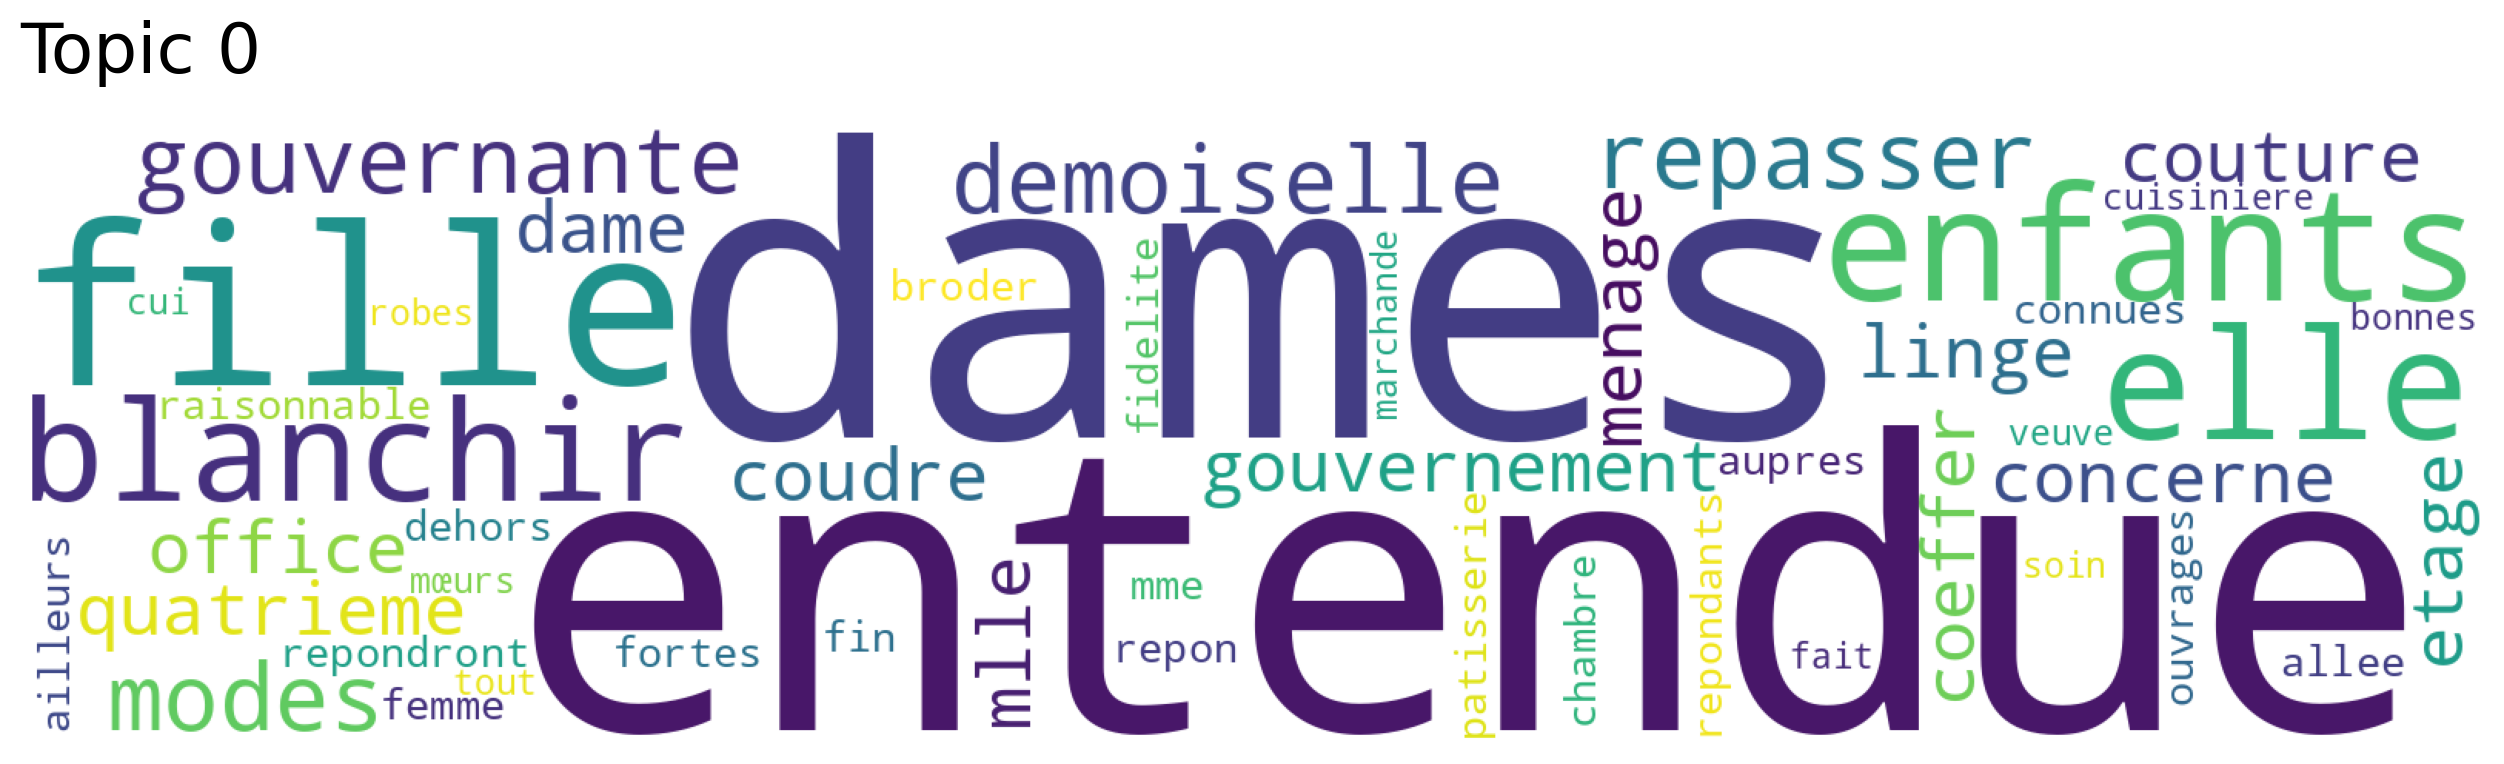
\includegraphics[width=12cm]{wordcloud_top2vec_0.png}
	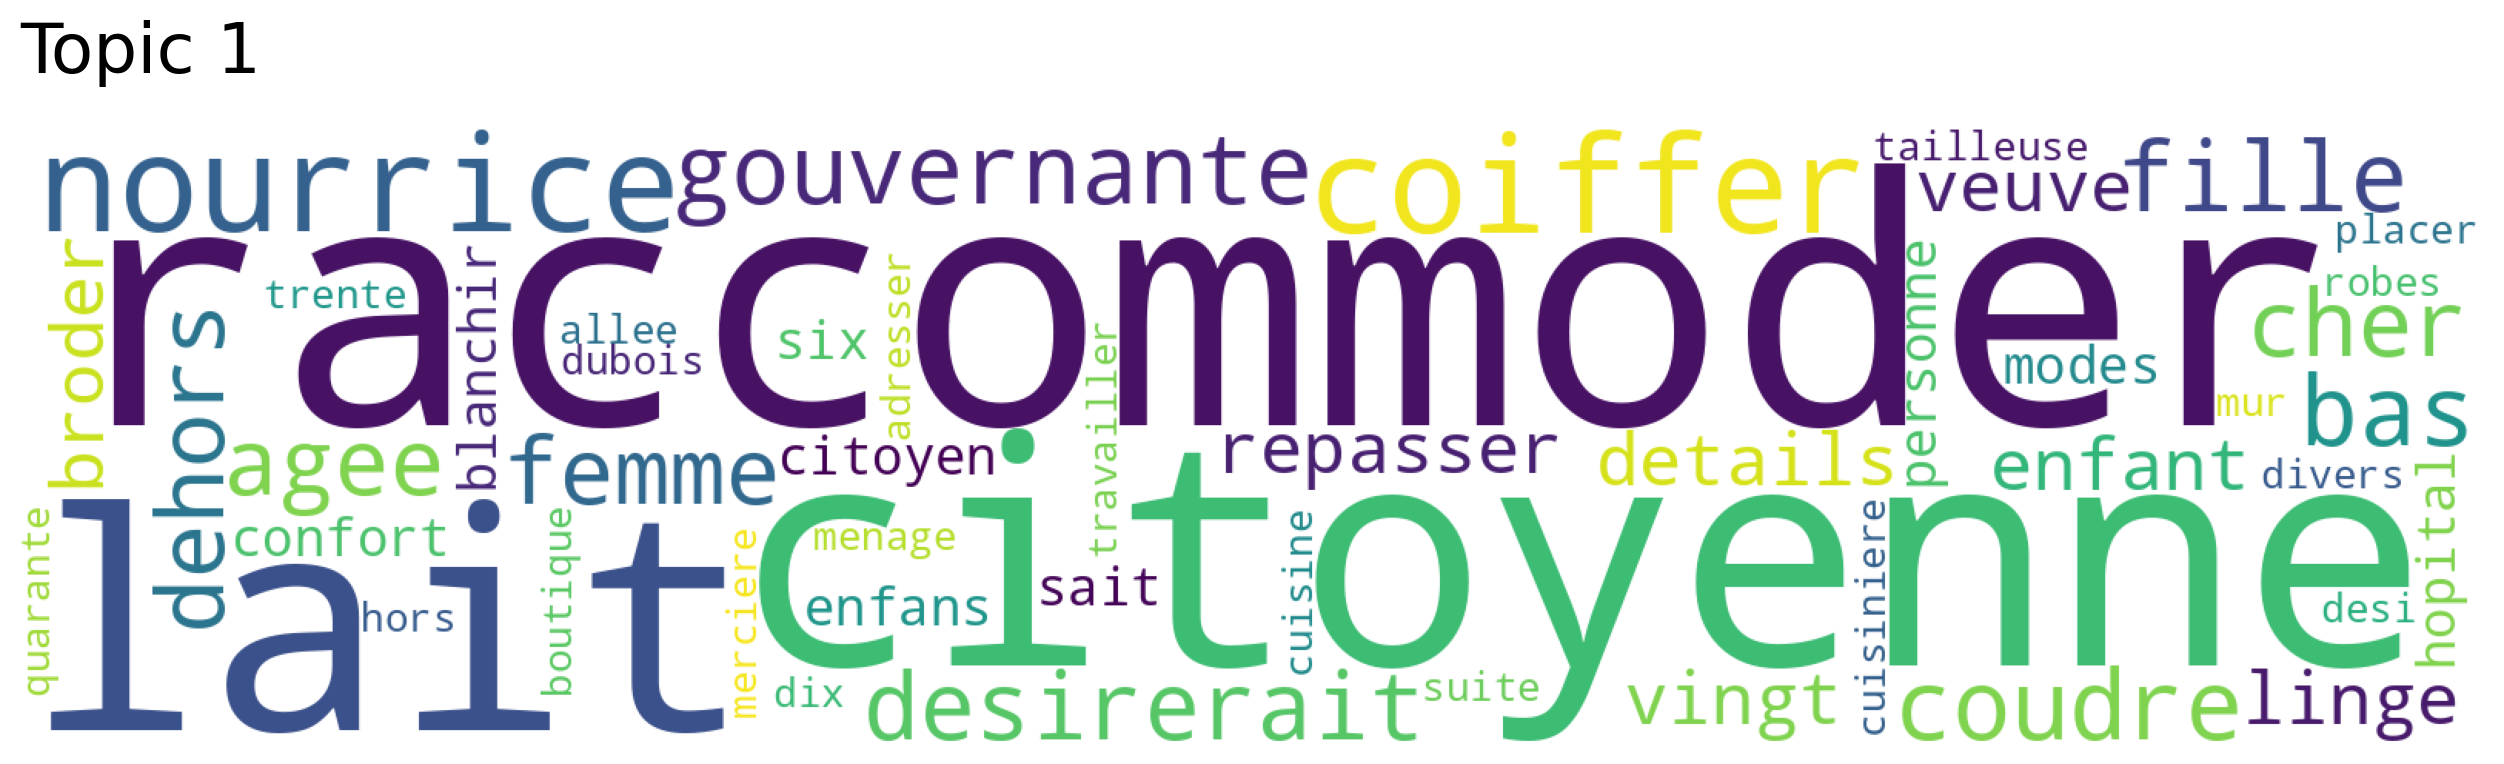
\includegraphics[width=12cm]{wordcloud_top2vec_1.png}
	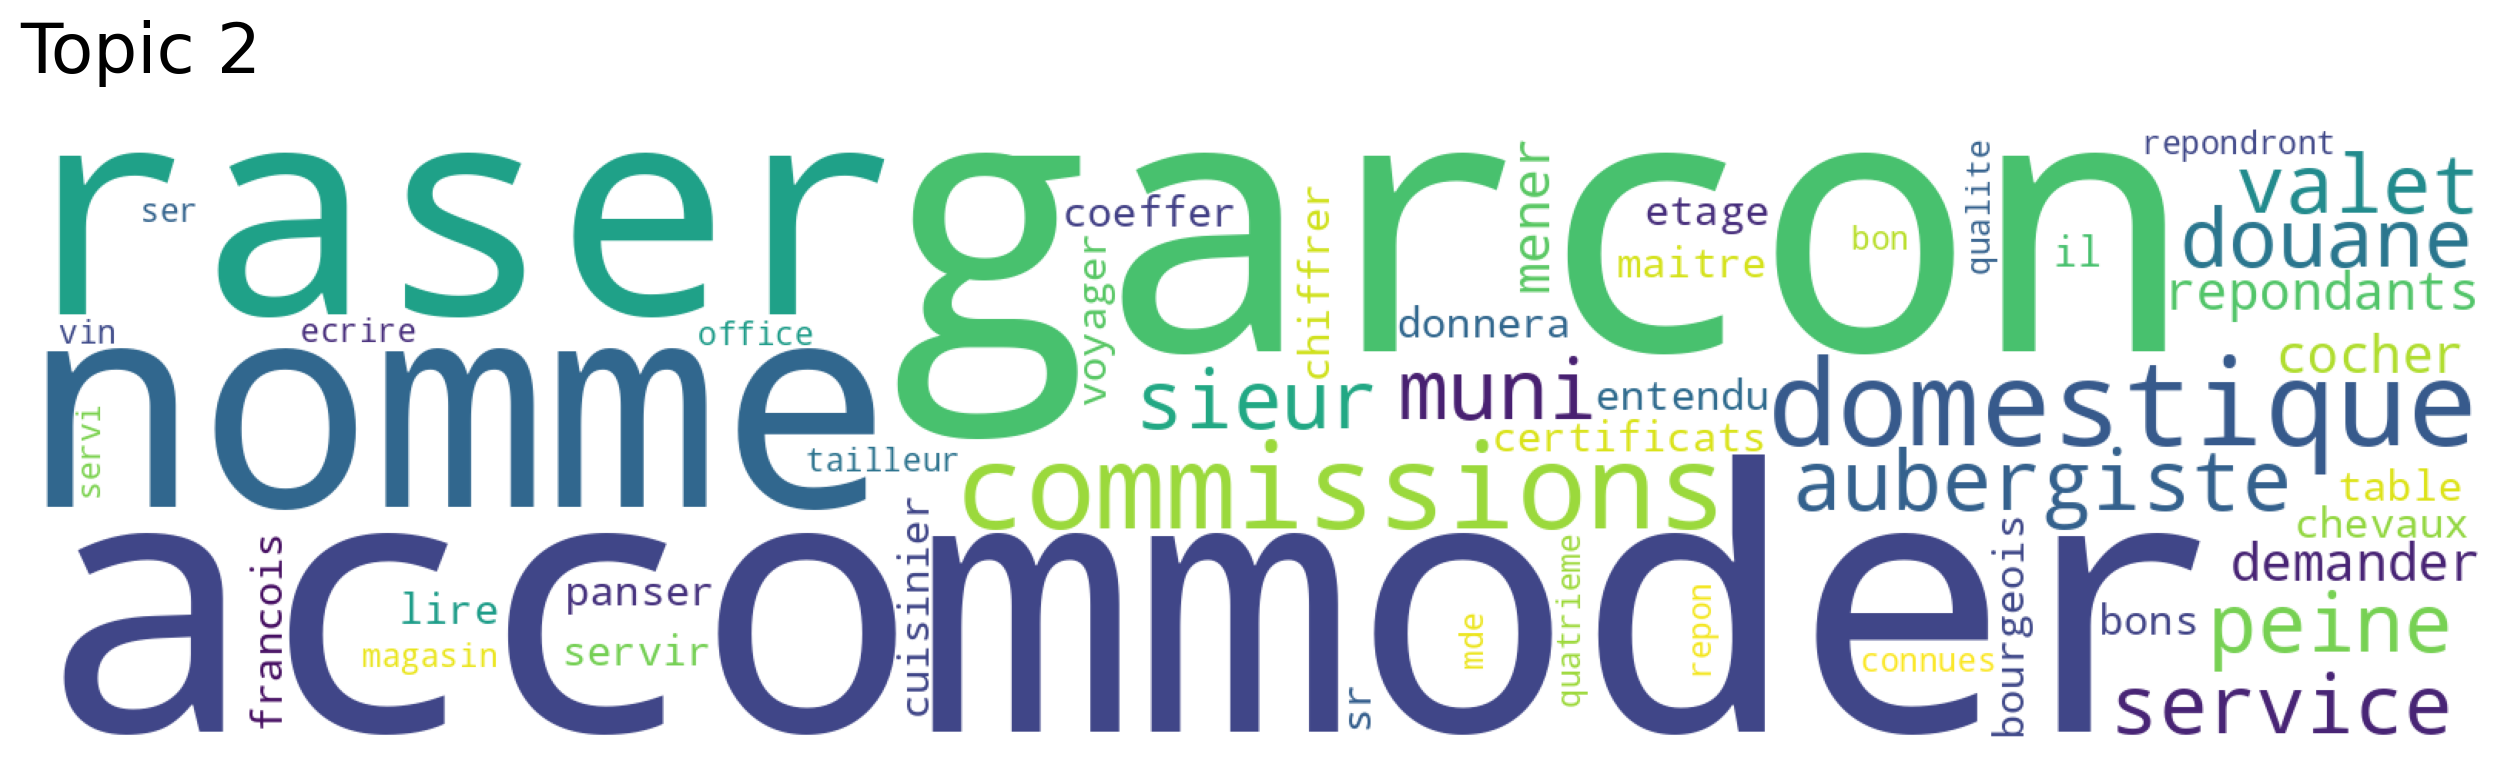
\includegraphics[width=12cm]{wordcloud_top2vec_2.png}
	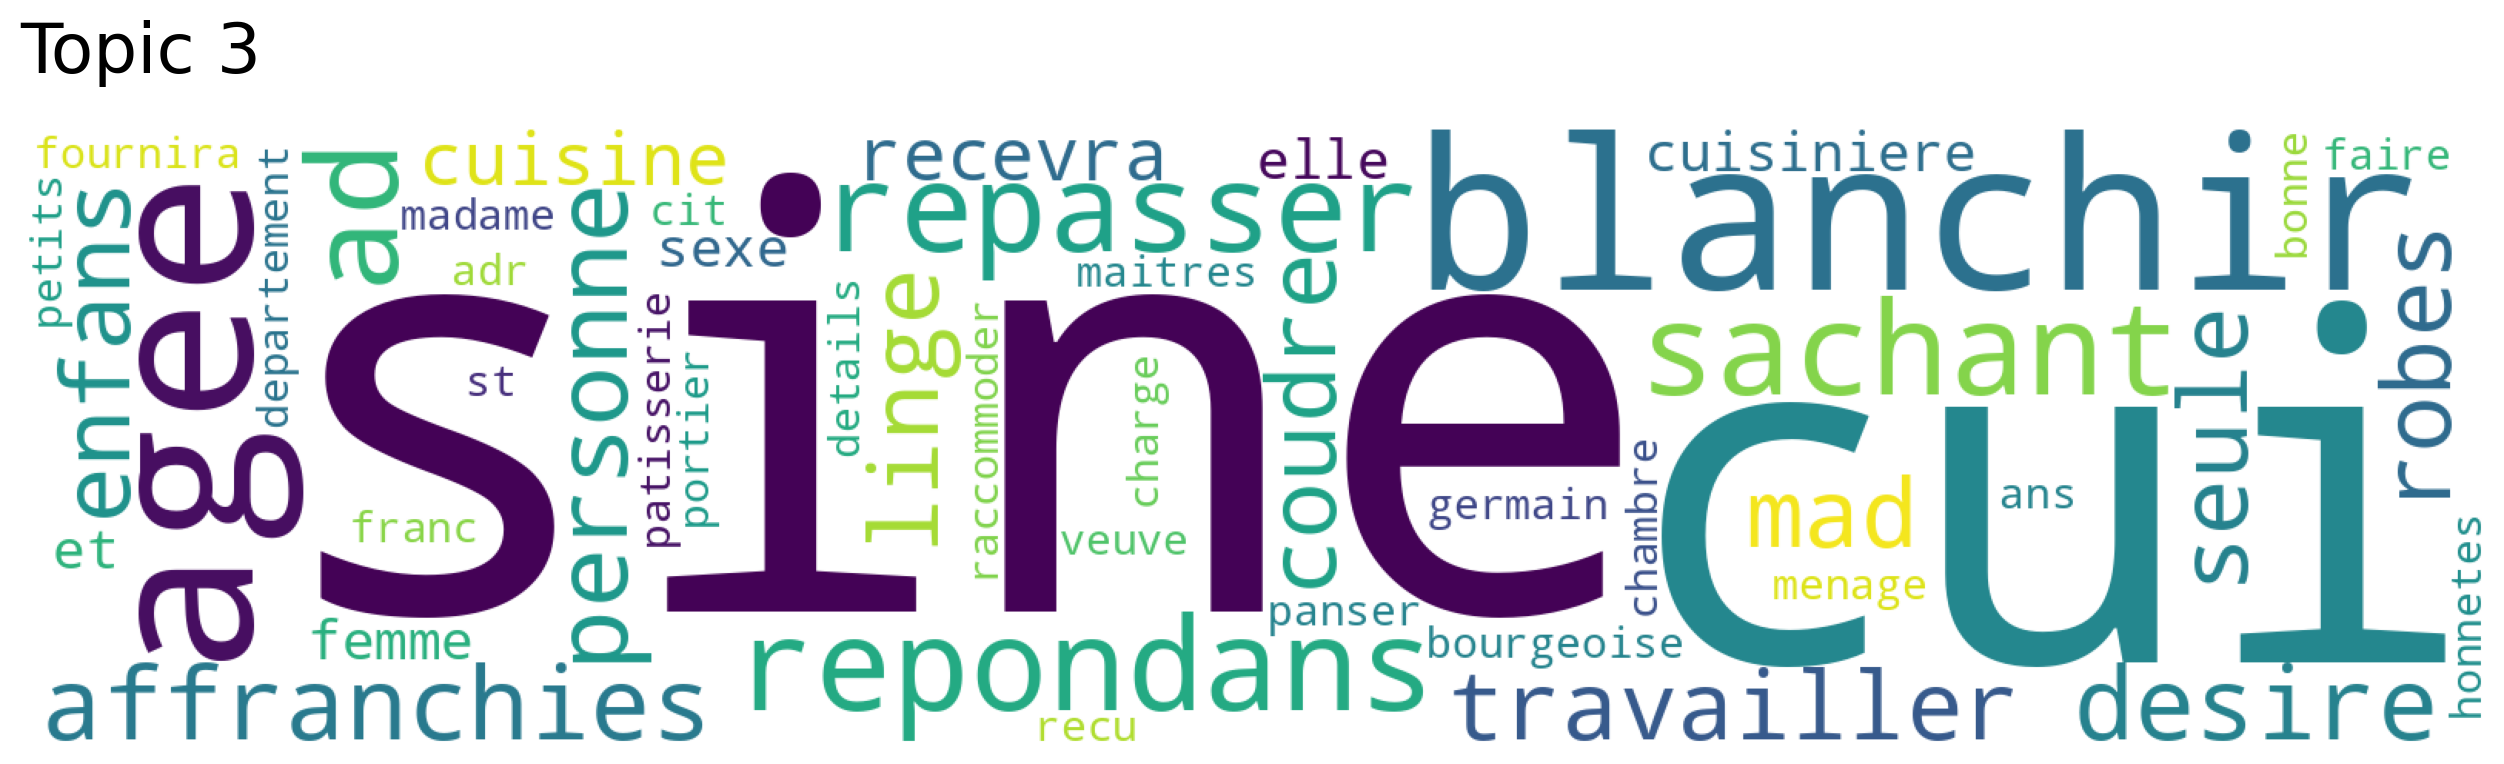
\includegraphics[width=12cm]{wordcloud_top2vec_3.png}
	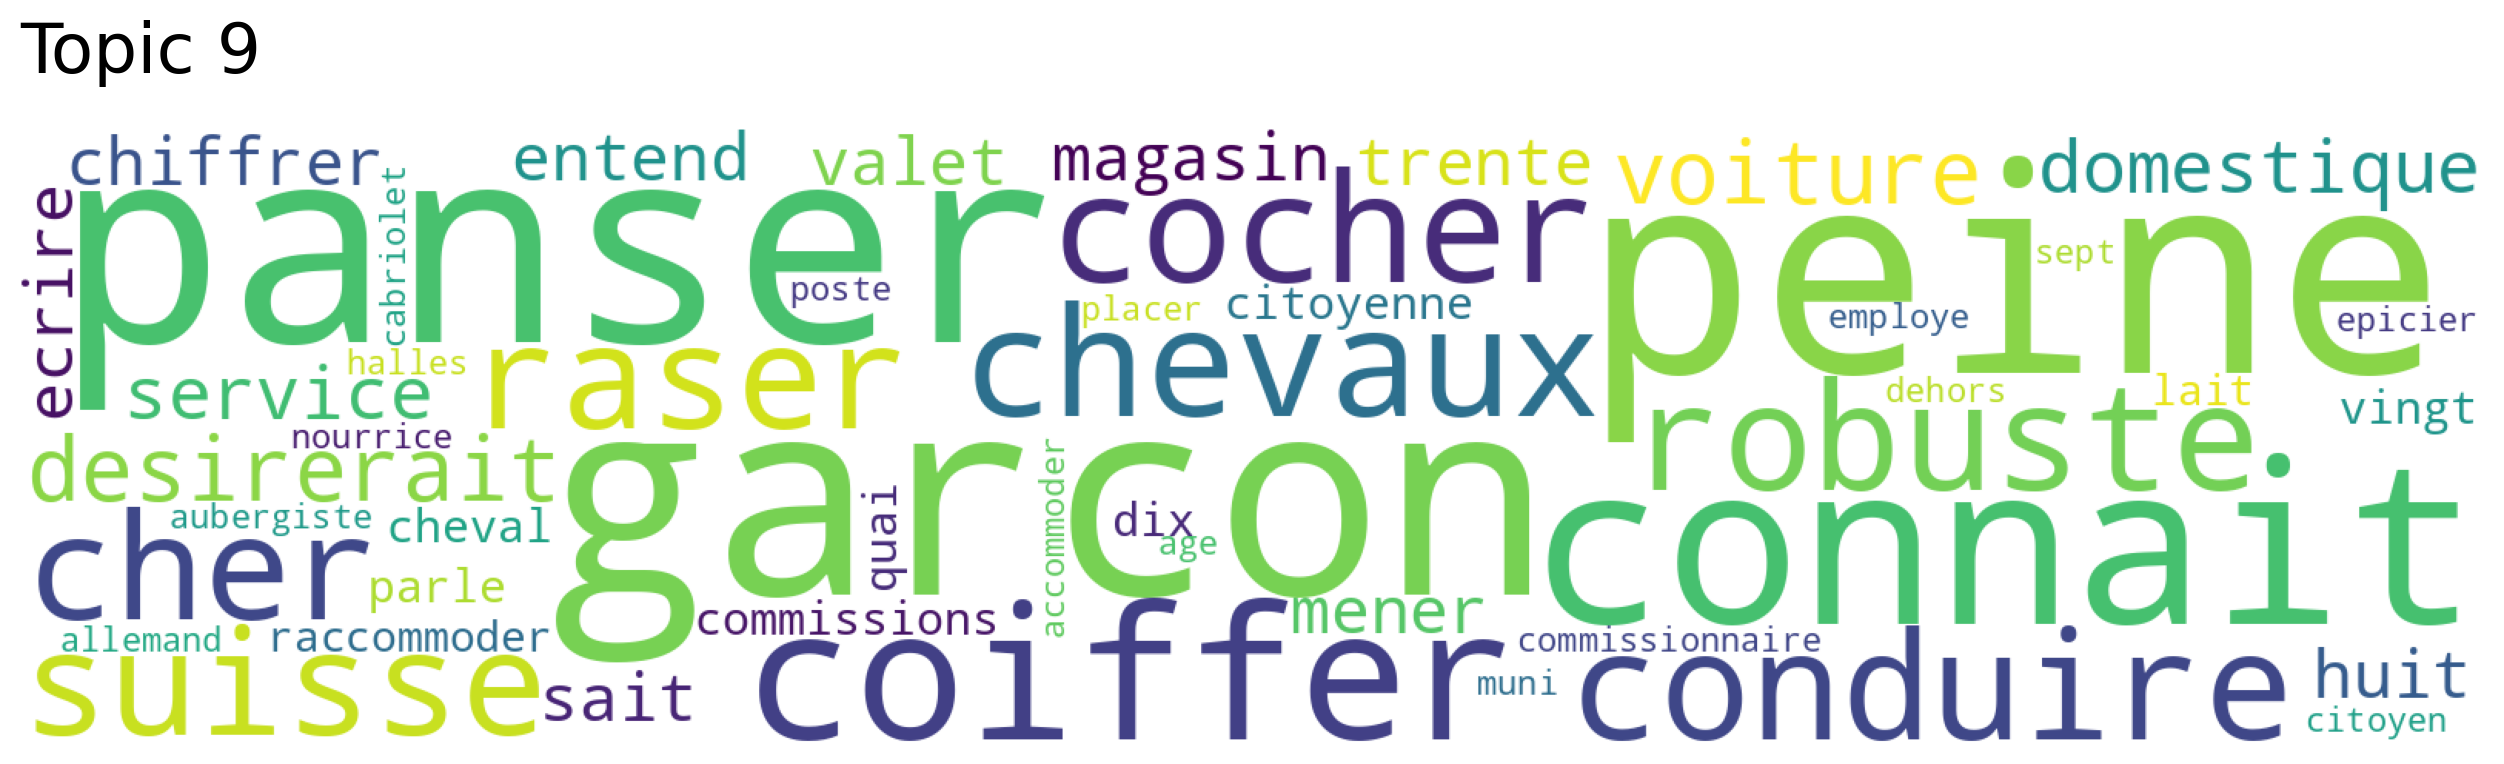
\includegraphics[width=12cm]{wordcloud_top2vec_9.png}
	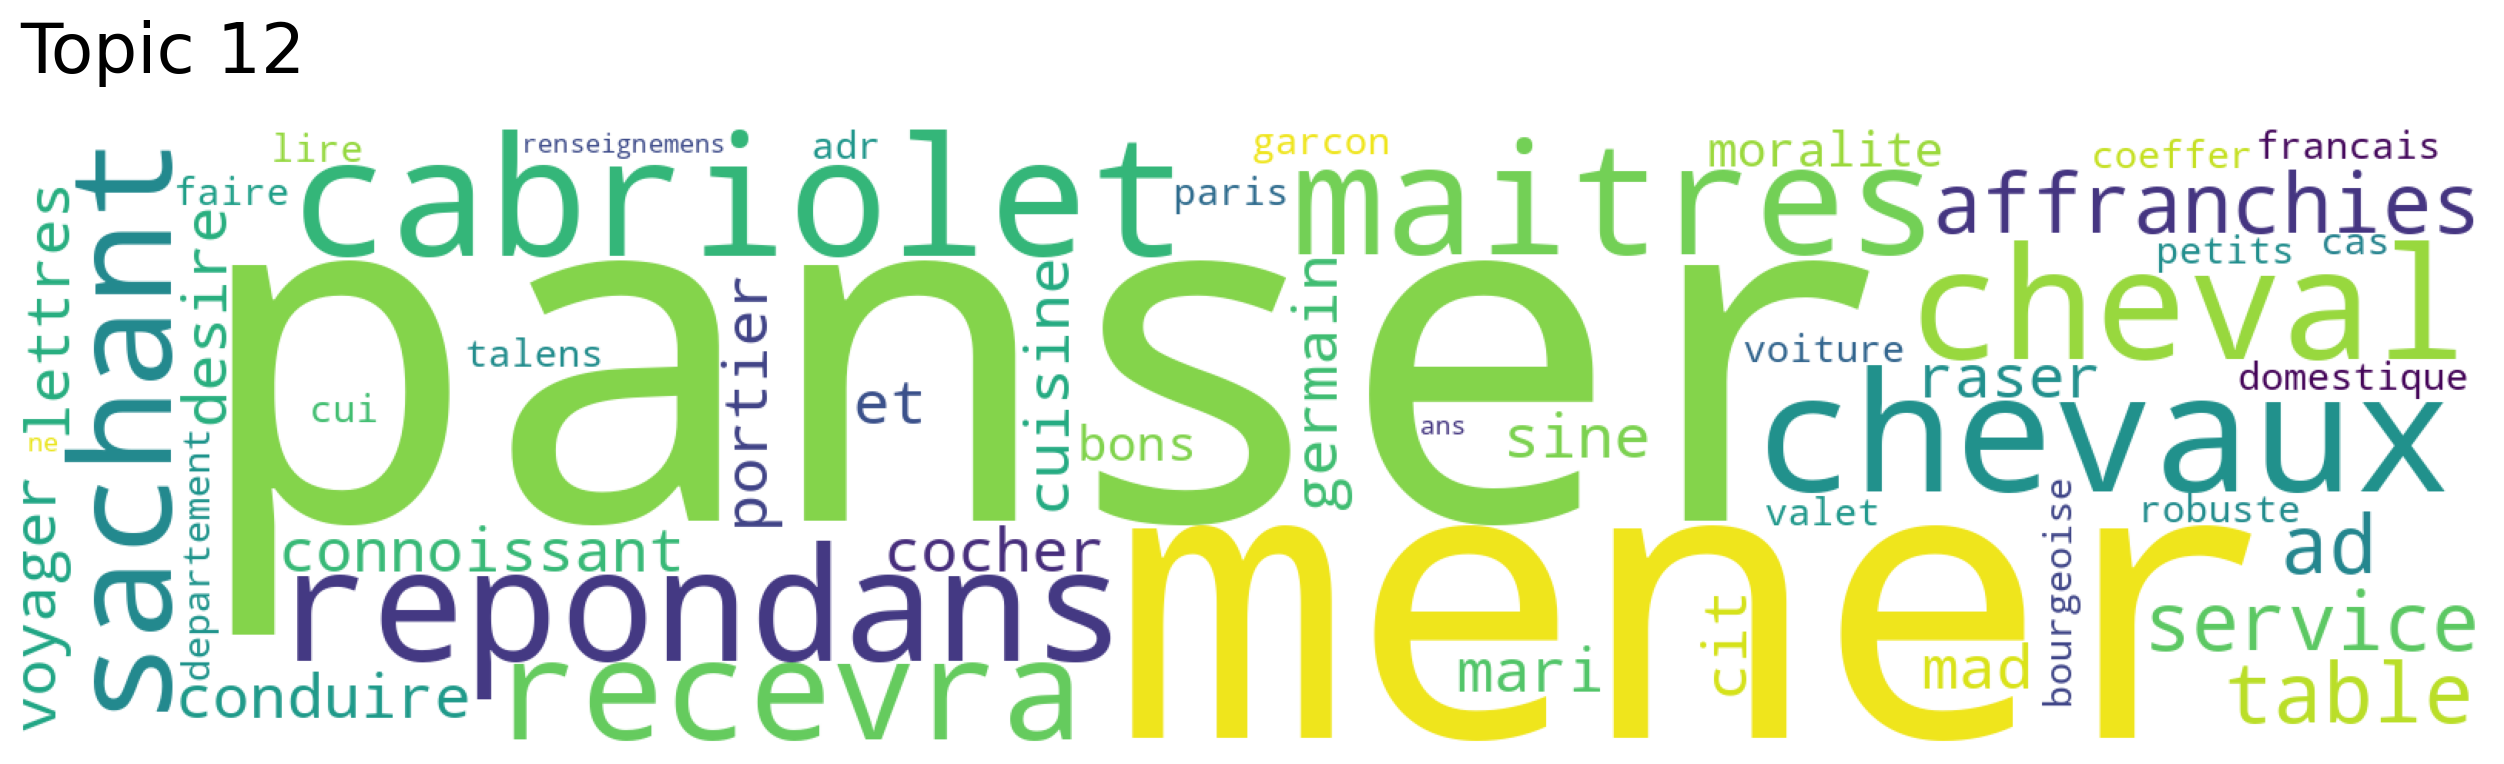
\includegraphics[width=12cm]{wordcloud_top2vec_12.png}
	\caption{Nuage de mots des topics relatifs au genre}
\end{figure}


Par ailleurs, Top2Vec permet également d'interroger la proximité (vectorielle) et donc la similarité (sémantique) des \textit{topics} générés avec d'autres mots, fournis par l'utilisateur, voire même de mots entre eux. Ainsi, les mots les plus similaires (similarité cosine) à "femme" sont, d'après le modèle, "linge" (0.58), "coudre" (0.57), "gouvernante" (0.54), "elle" (0.51) et repasser (0.49). Les mots les plus similaires à "homme" incluent "garçon" (0.48), "conduite" (0.43), "marchand" (0.42) et "affaires" (0.38).

\section{... et révélateurs de la spécificité de la population des annonces}

En plus de confirmer la répartition sexuée du travail au sein des annonces, les\textit{ topics} générés par Top2Vec sont également sensibles à la particularité de certaines annonces, qu'on a déjà étudiées: il s'agit des annonces proposant les services d'une domesticité intellectuelle, qualifiée et spécialisée, parmi lesquels se trouvent précepteurs, secrétaires ou chargés d'affaires. 

Le modèle Top2Vec non seulement les isole des annonces et des compétences plus manuelles, mais divise cette domesticité par spécialisation: le topic 4 est consacré à l'enseignement (histoire, géographie, latine, principes, précepteur); on peut d'ailleurs y percevoir le poids des ecclésiastiques dans l'éducation des jeunes de grande famille. Le topic 6 concerne plutôt le commerce, la gestion des affaires et des terres ou la tenue des comptes (changes, livres, tenir, commerce...), rôle qui incombe généralement au régisseur, au notaire ou à l'homme d'affaires. Enfin, le topic 13, en réunissant les mots "commis", "secrétaire", "plume" et "écriture", semble plutôt désigner les domestiques particuliers du maître, qui sont chargés entre autres de sa correspondance. 

\begin{figure}[h!t]
	\centering
	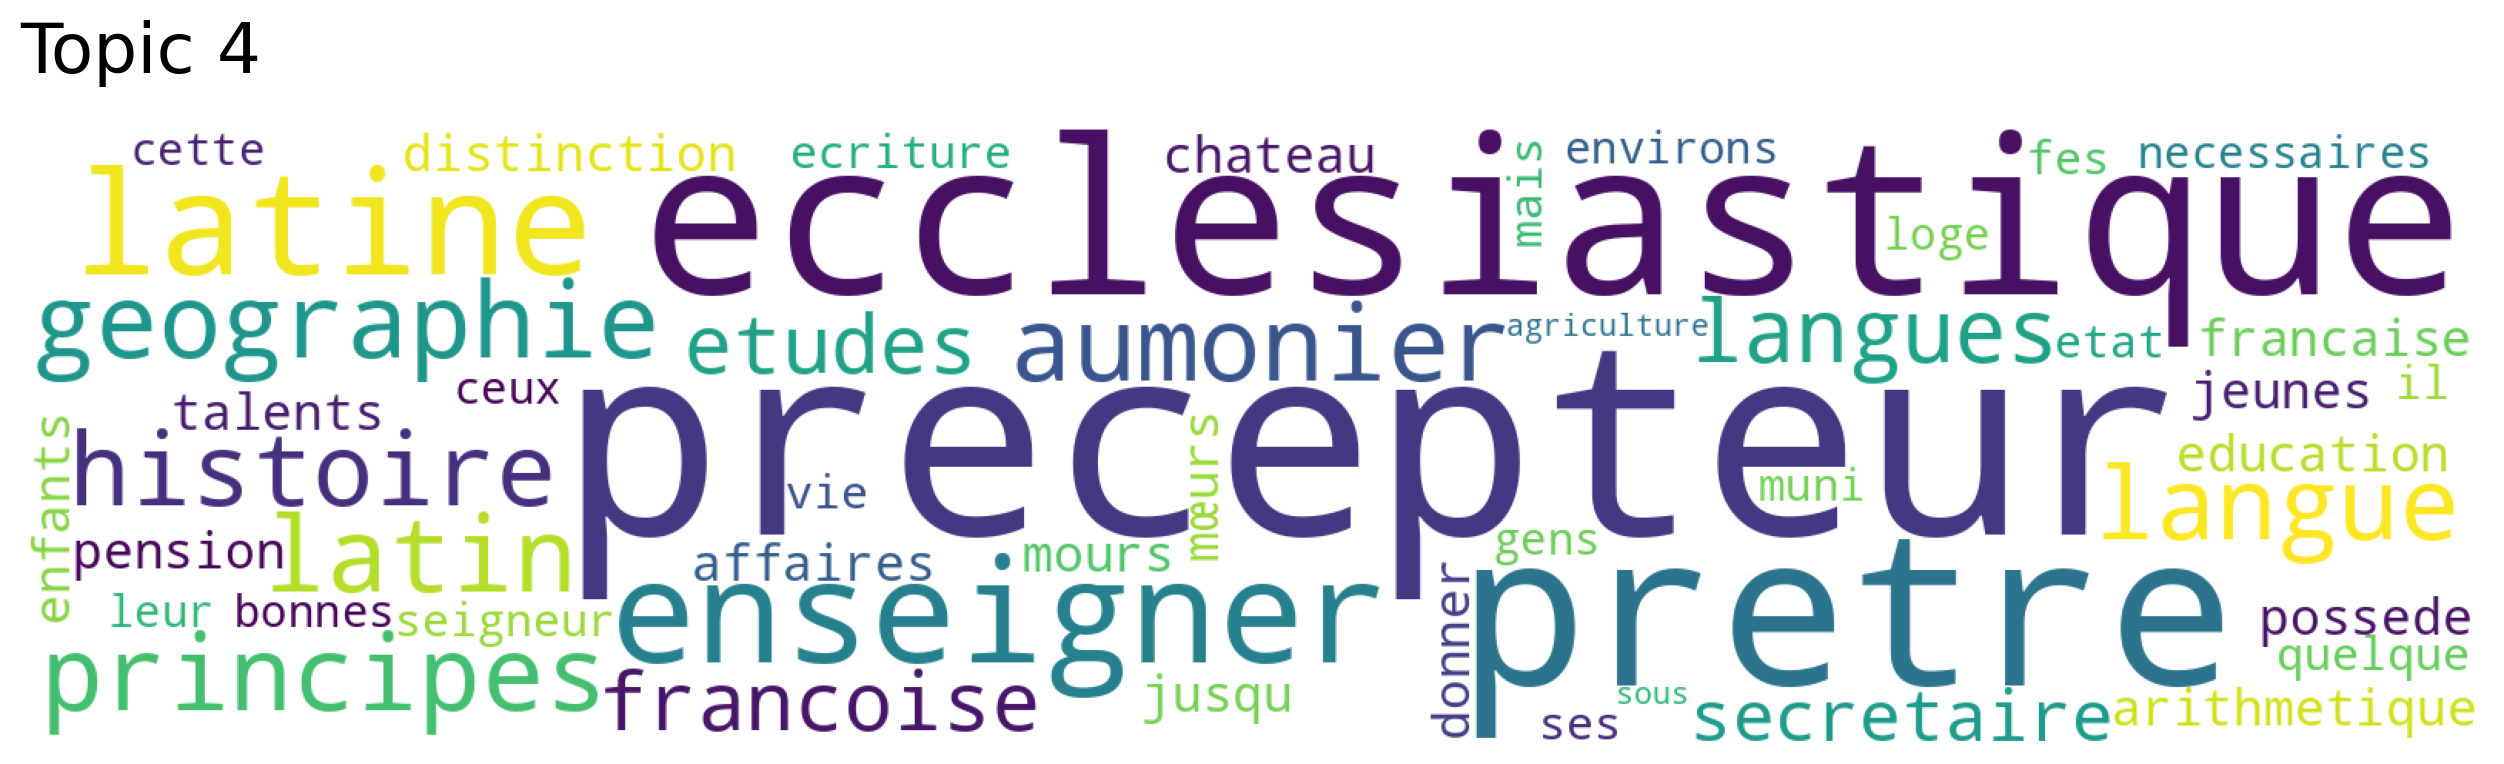
\includegraphics[width=12cm]{wordcloud_top2vec_4.png}
	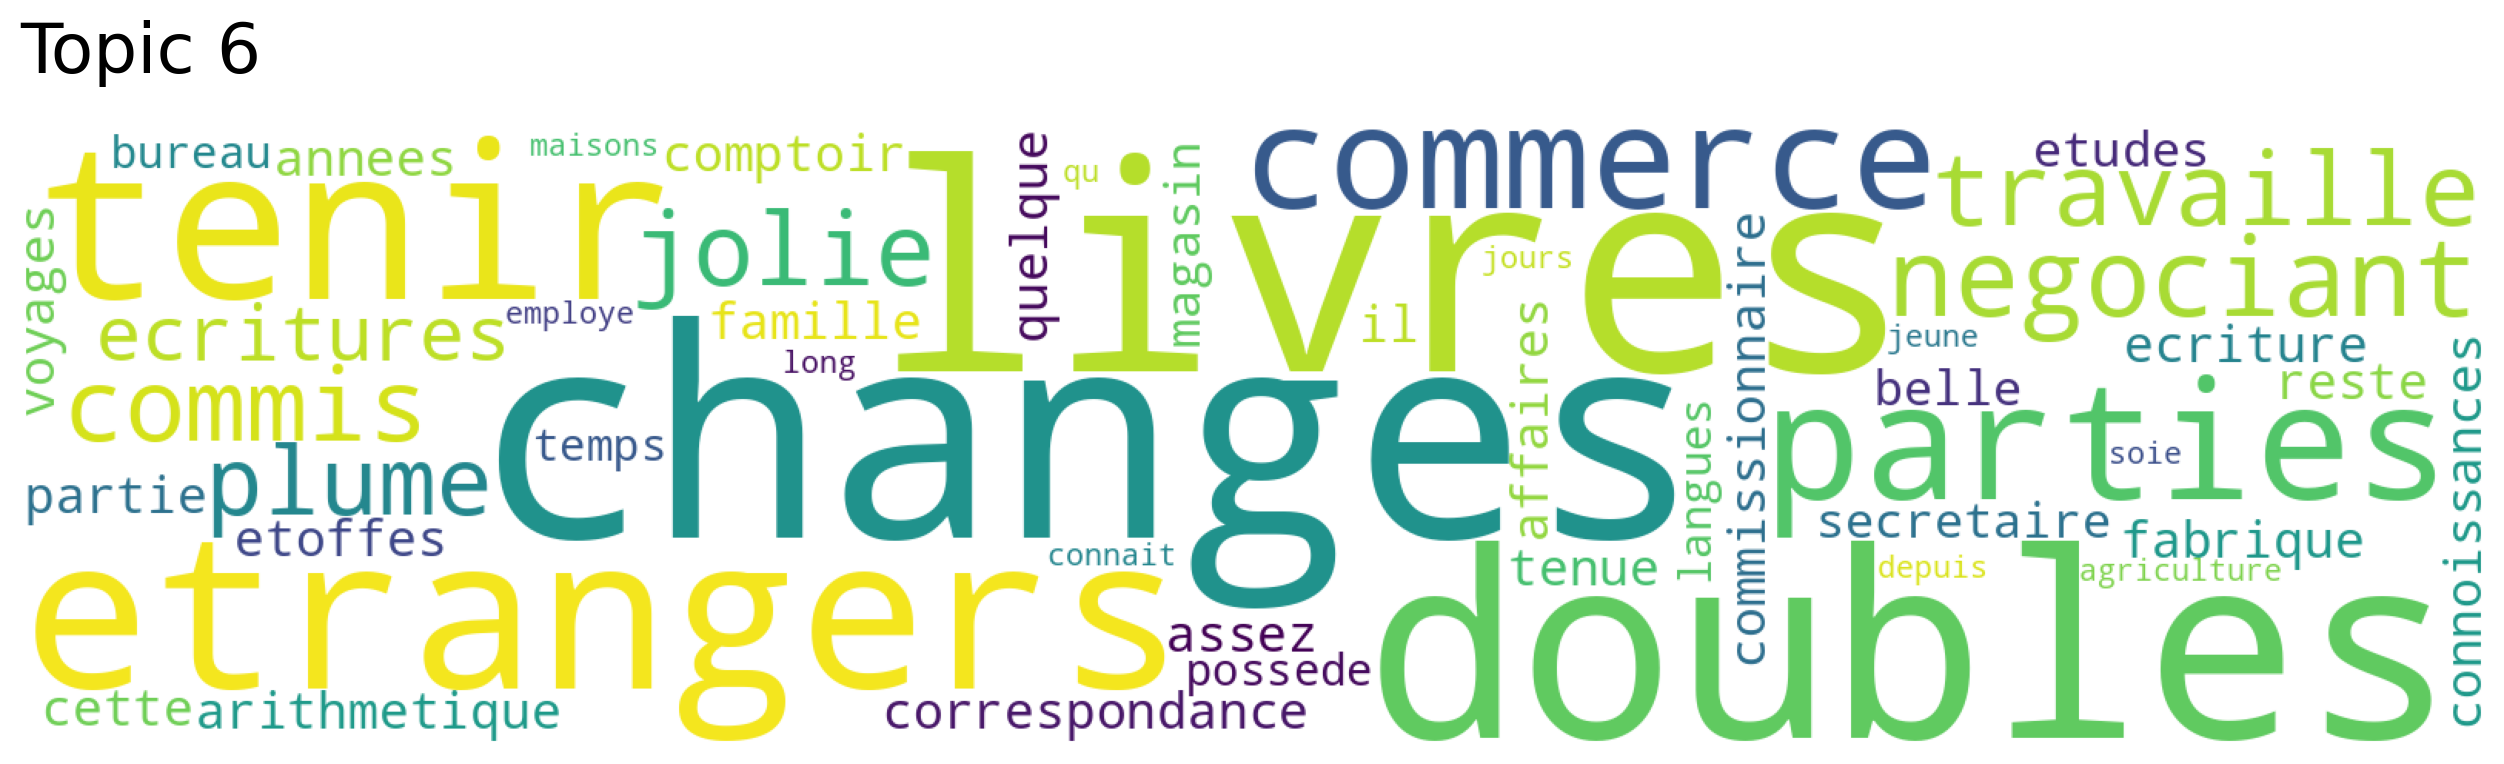
\includegraphics[width=12cm]{wordcloud_top2vec_6.png}
	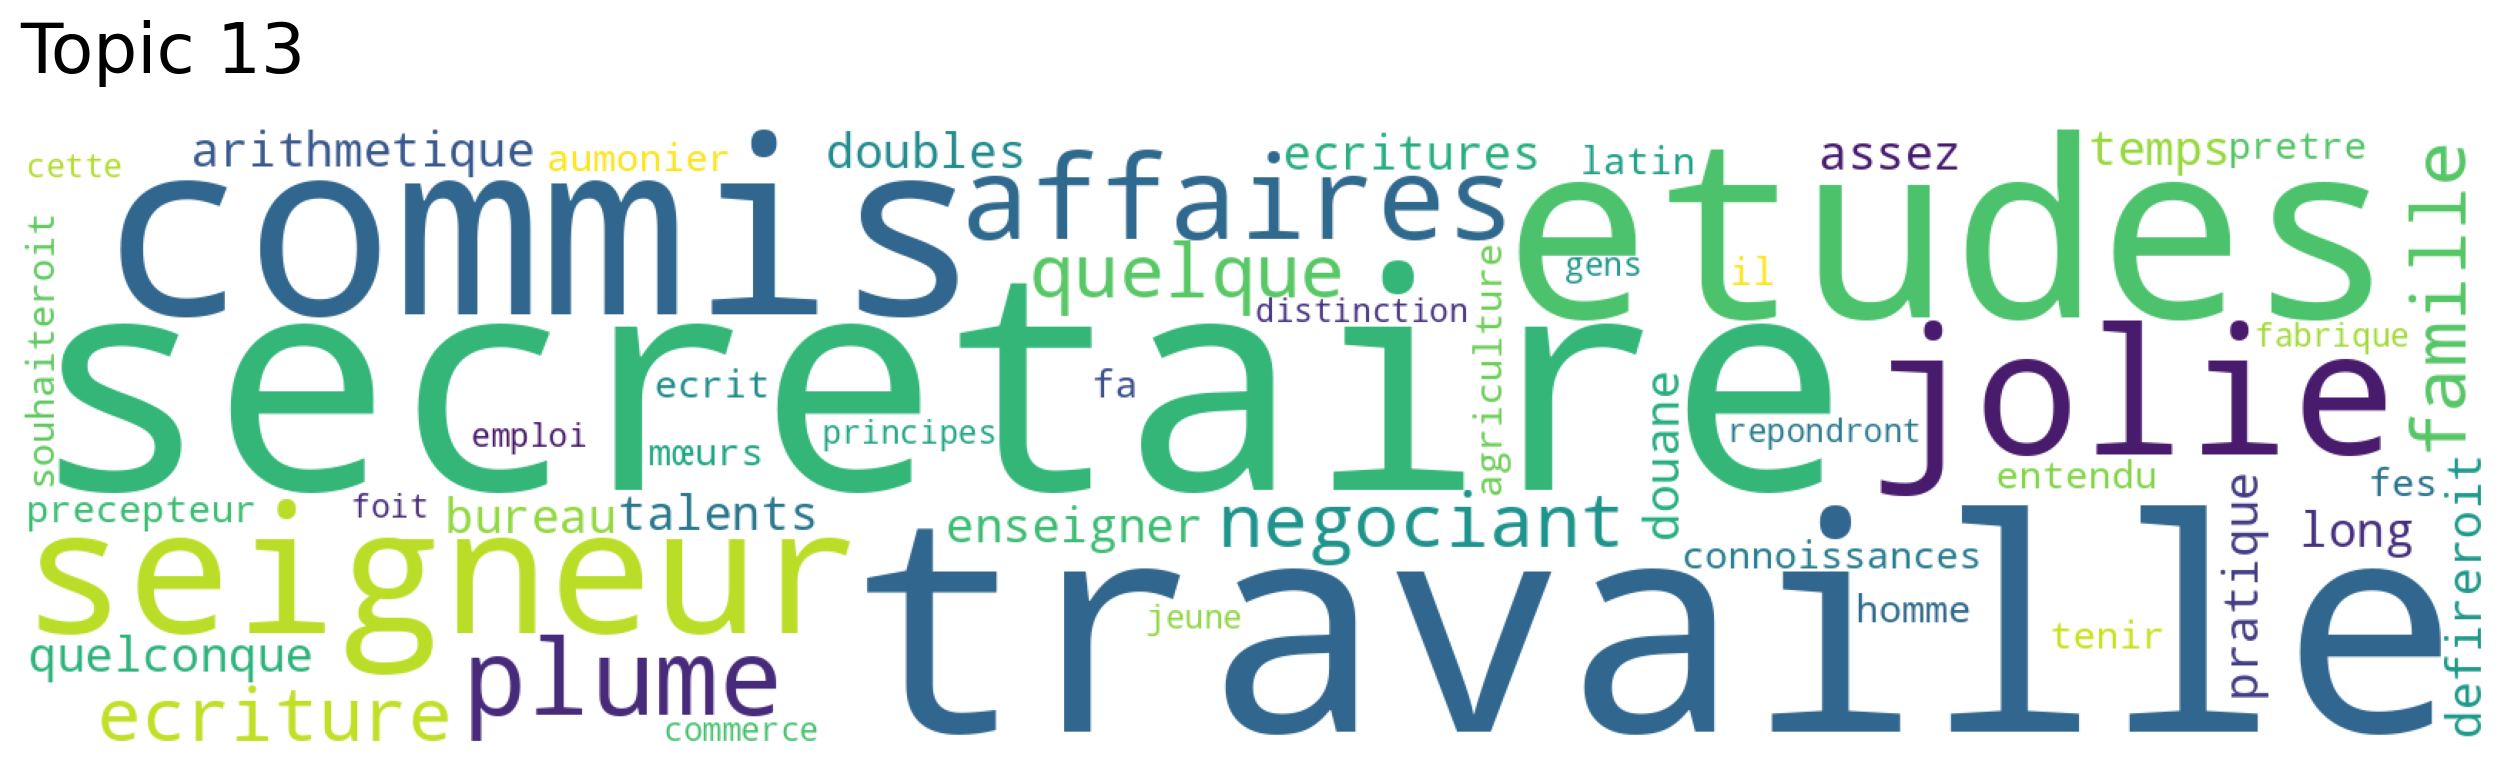
\includegraphics[width=12cm]{wordcloud_top2vec_13.png}
	\caption{Nuage de mots des topics relatifs à la domesticité qualifiée}
\end{figure}

\section{\textit{Topics} et division sociale du travail}

Mais les thèmes générés par le modèle révèlent également un panorama plus large du travail urbain à l'époque moderne, qui rencontre ou recouvre parfois le champ strict de la domesticité. Le topic 10 notamment, dédié au commerce et au travail de boutique (fabrique, étoffes, soie, négociant, fabricant, ...), montre que les annonces déposées ne concernent pas uniquement la domesticité privée; être commis ou fille de boutiques sont également des horizons possibles pour les jeunes gens sans condition. Il s'agit d'un résultat que j'ai eu du mal à déceler avec les méthodes employées jusqu'ici (hormis la présence de "commis" parmi les emplois extraits du corpus) mais qui est révélé grâce au \textit{topic modeling}.

De même, le topic 16 se réfère également au commerce mais lui ajoute cette fois une dimension itinérante (voyages, correspondance), rappel que "les grandes villes agissent comme des plaques tournantes d’un marché du travail dont le périmètre peut transcender le continent européen\footcites{kramplAdresserClercHuissier2017}". 

\begin{figure}[h!t]
	\centering
	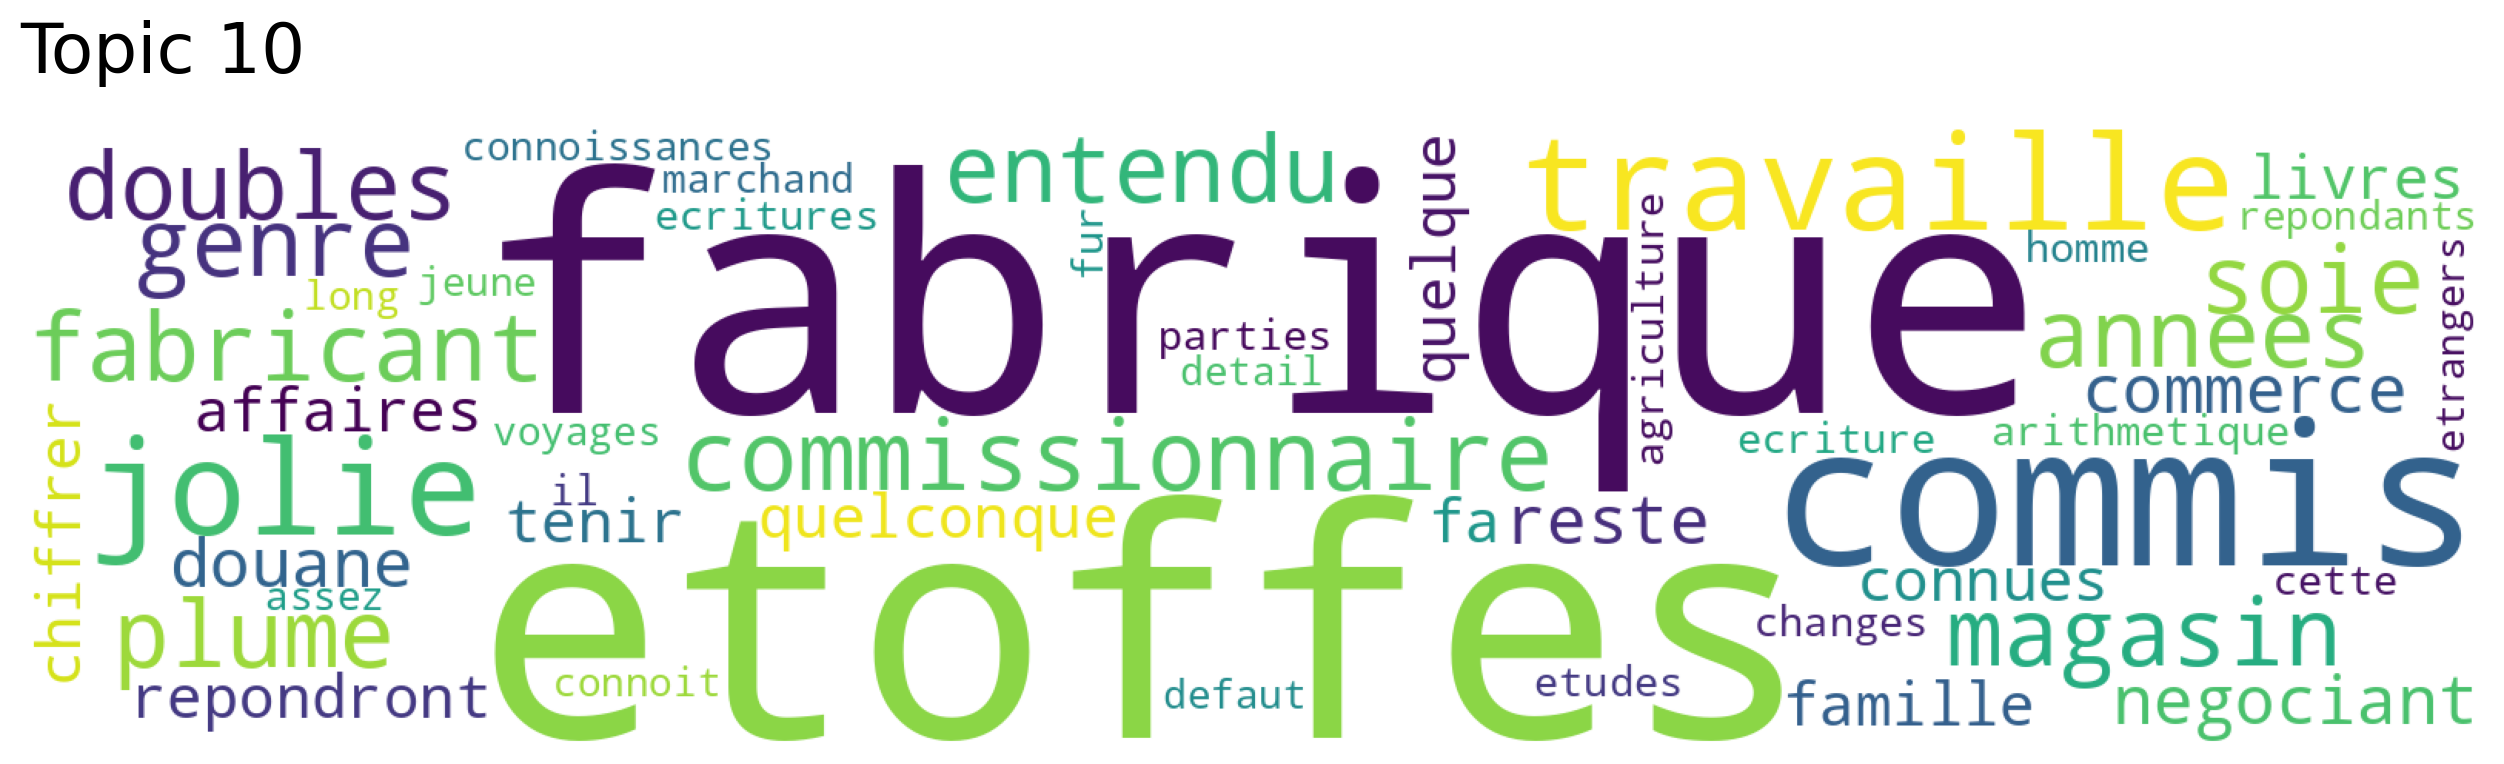
\includegraphics[width=12cm]{wordcloud_top2vec_10.png}
	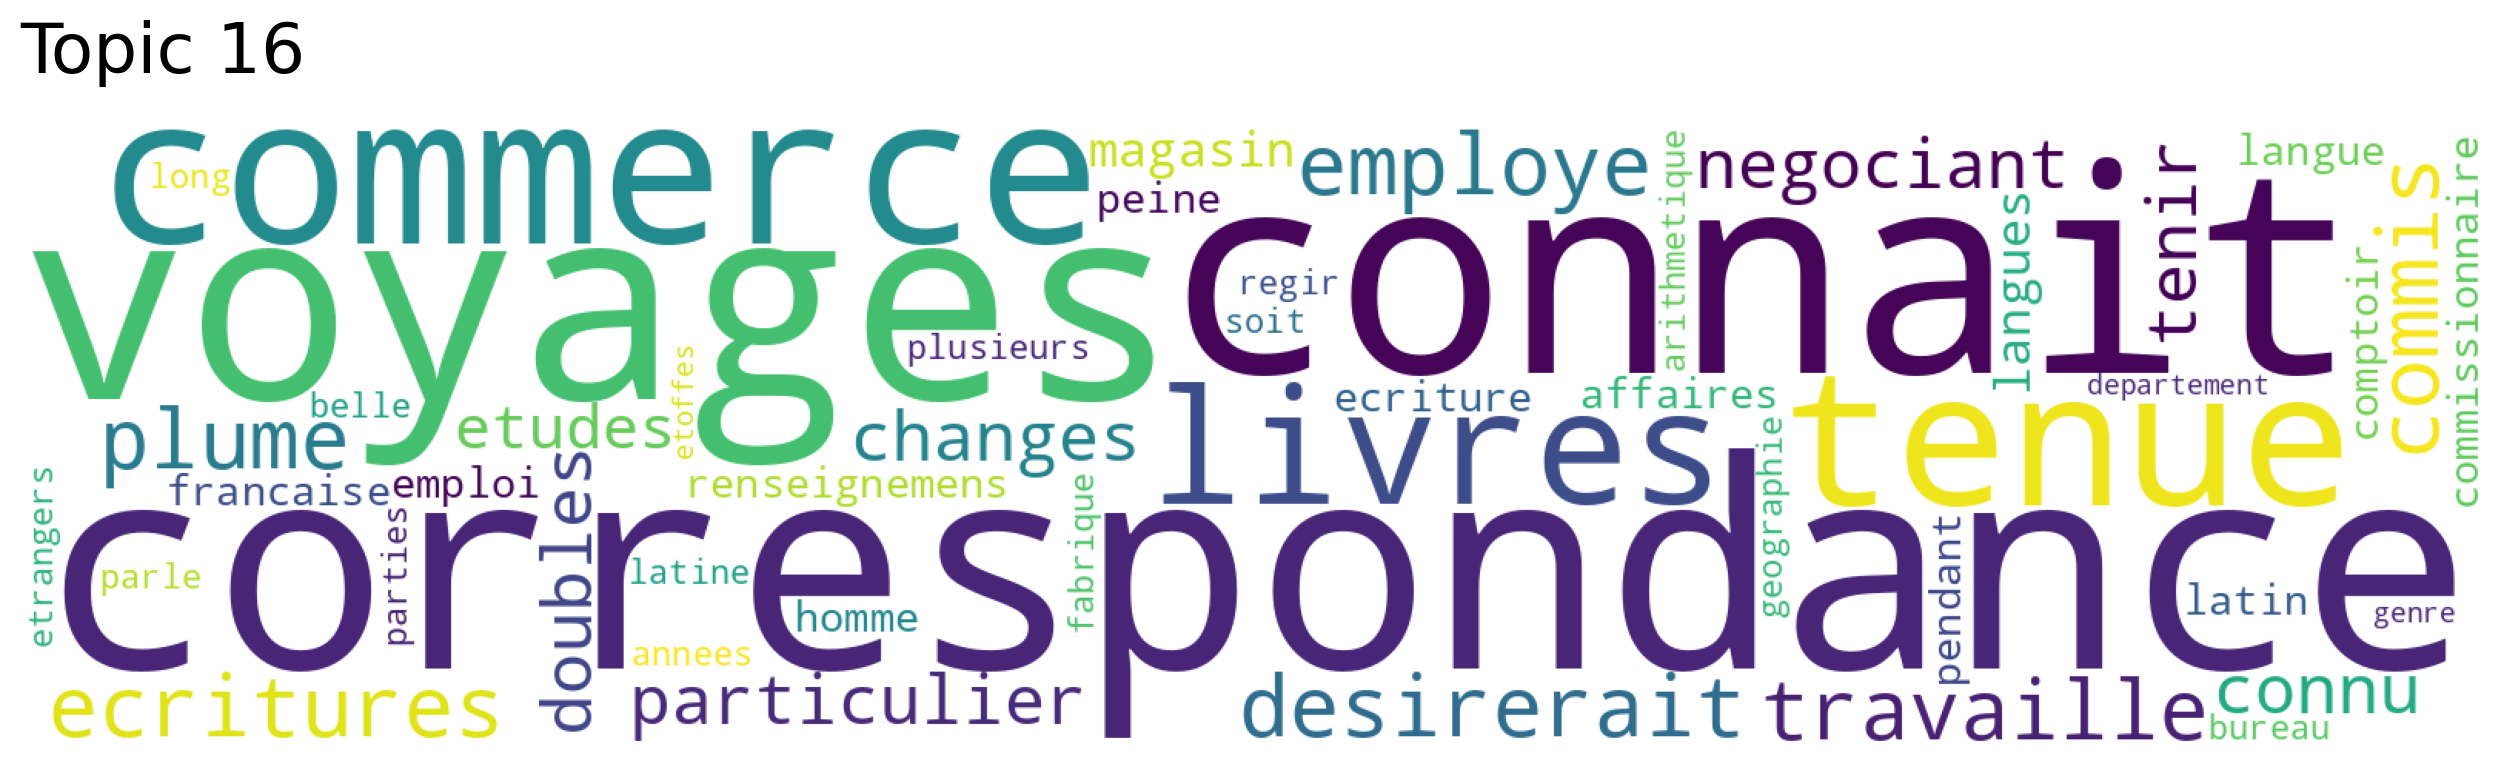
\includegraphics[width=12cm]{wordcloud_top2vec_16.png}
	\caption{Nuage de mots des topics 10 et 16}
\end{figure}

\section{Dévoiler les anomalies du corpus}

Enfin, le \textit{topic modeling}, en associant entre elles les annonces les plus similaires sémantiquement, permet aussi de faire apparaître des anomalies ou des exceptions du corpus, qui seraient autrement passées inaperçues. Ainsi, le topic 5, qui se réfère aux chaises de poste et aux offres de transport (voiture, frais, partir, voyage) est la preuve que ma tentative d'éliminer ces annonces parasites dans le corpus initial a en partie échouée. Ce faisant, le \textit{topic} renseigne indirectement sur l'importance des annonces prenant pour objet le voyage et le "covoiturage"; le journal devient là aussi un support incontournable créant de nouvelles configurations d'intermédiation des personnes\footcites{zellerAuxOriginesCovoiturage2018}. 

\begin{figure}[h!t]
	\centering
	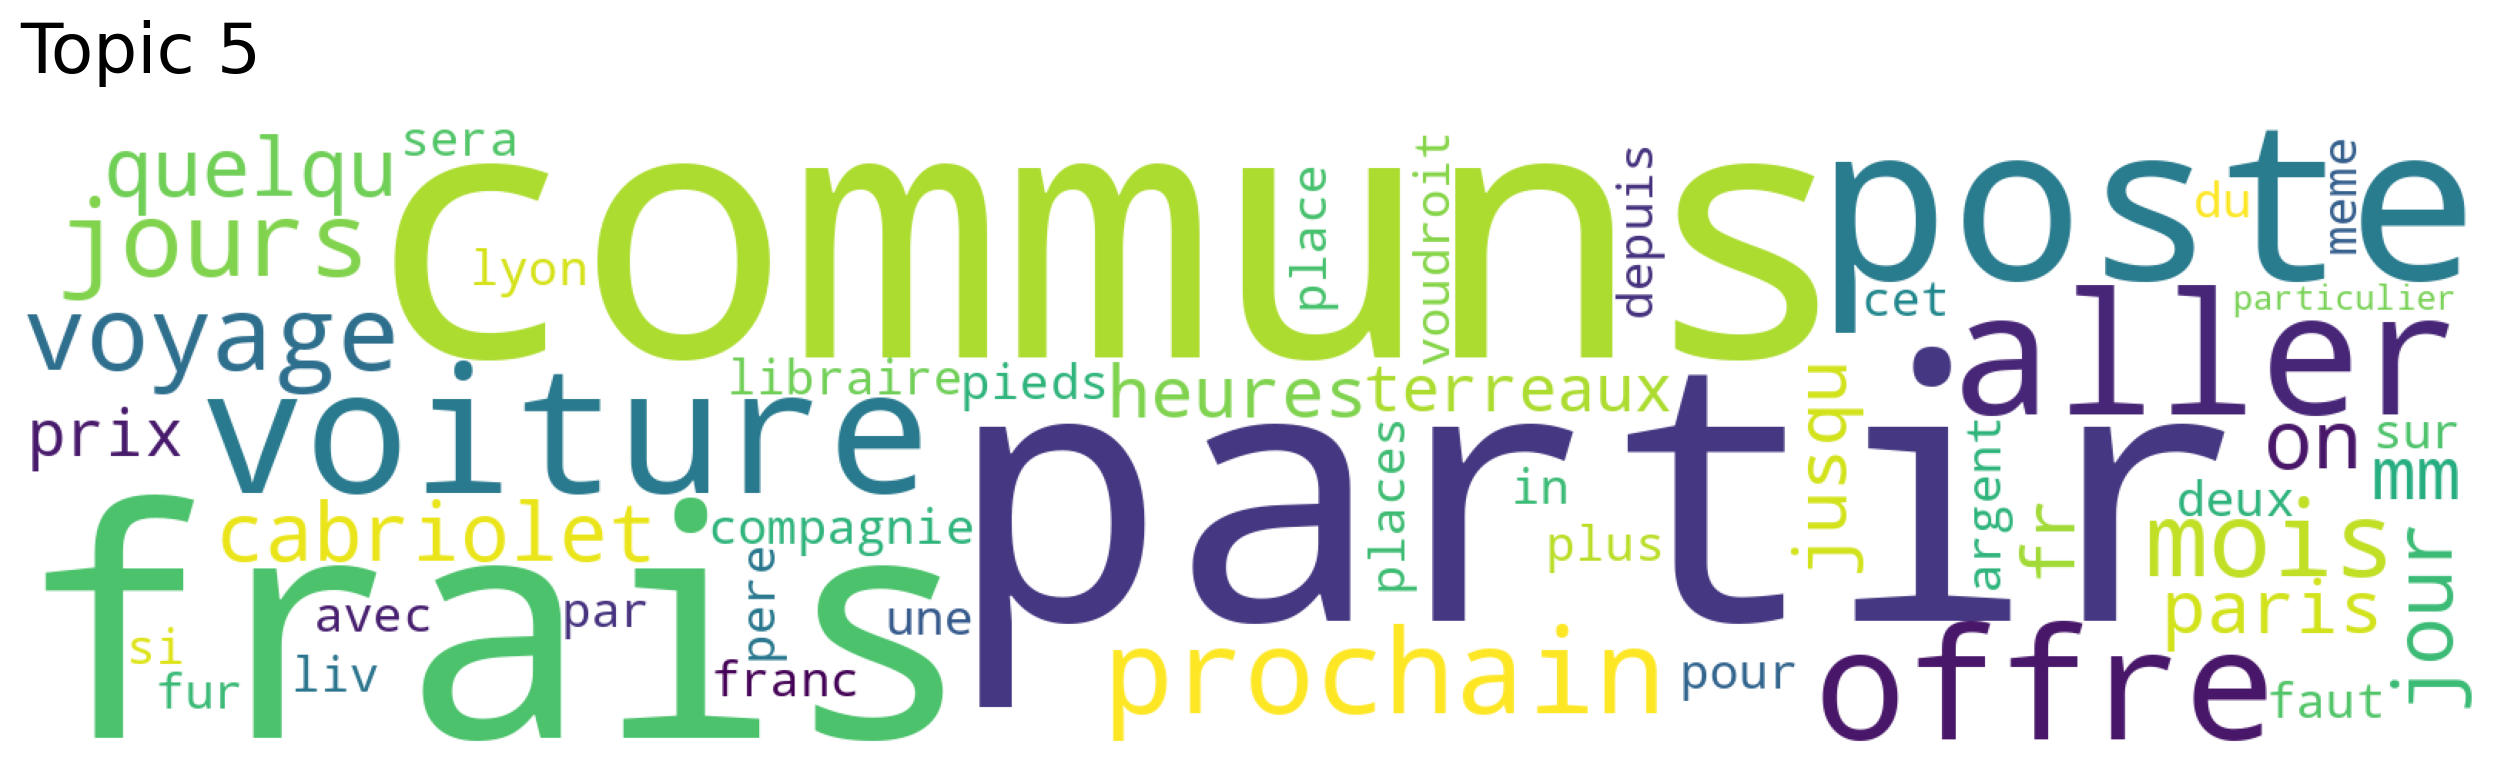
\includegraphics[width=12cm]{wordcloud_top2vec_5.png}
	\caption{Nuage de mots du topic 5}
\end{figure}



\chapter{Modéliser les \textit{topics} dans l'espace social avec BERTopic}

\section{Méthode}

L'algorithme de BERTopic\footnote{Documentation disponible sur le github de BERTopic: \url{https://maartengr.github.io/BERTopic/index.html}}, le troisième et dernier outil de \textit{topic modeling} que j'ai utilisé dans le cadre de cette étude, est par beaucoup d'aspects similaire à celui de Top2Vec: comme lui, il repose sur des \textit{embeddings} et des \textit{clusters} de mots, ne nécessite pas de \textit{pre-processing} des données, procède ensuite à une réduction de dimensionnalité à l'aide de la technique UMAP (\textit{Uniform Manifold Approximation and Projection}), et détermine seul le nombre de \textit{topics} à générer. 

Néanmoins, certaines différences existent entre les deux algorithmes, notamment relatives à la façon dont les clusters sont considérés. Alors que Top2Vec crée des \textit{topics} à partir \textit{clusters} de mots, les mots les plus proches du centre du cluster étant alors les plus représentatifs du topic, BERTopic assemble tous les mots d'un cluster pour en faire un seul document, dont il extrait ensuite les éléments les plus représentatifs à l'aide d'une mesure Tf-Idf (\textit{Term Frequency - Inverse Document Frequency}. Les termes les plus pertinents sont donc ceux qui auront le plus grand nombre d'occurrences dans un document (\textit{Term Frequency}), rapportés à leur rareté relative dans le corpus (\textit{Inverse Document Frequency}). Ainsi, des mots très courants dans l'ensemble des documents du corpus (les mots-vides, par exemple) ont peu de chances d'être considérés comme pertinents; en revanche, un mot rare à l'échelle du corpus, mais présent plusieurs fois dans un même document, a beaucoup de chances d'être sélectionné. 

Par ailleurs, BERTopic permet, contrairement à Gensim ou Top2Vec, de concaténer les \textit{topics} par classe (dans notre cas, par ville par exemple) et de réaliser un \textit{topic modeling} dynamique, permettant de visualiser les évolutions du poids des \textit{topics} dans le temps. Pour mobiliser ces deux possibilités offertes par l'algorithme, j'ai au préalable créé deux nouveaux \textit{datasets} plus équilibrés, le premier en sélectionnant aléatoirement mille annonces de chaque ville (au total, 3000 annonces), et le second en sélectionnant cent annonces pour chaque année de publication (au total, 3900 annonces). 

\section{Aperçu général des \textit{topics}: beaucoup de similarités avec Top2Vec, quelques différences}


Le modèle généré à partir du corpus d'origine a permis de distinguer vingt-quatre \textit{topics}, soit autant qu'avec Top2Vec. Parmi ceux-ci, on observe beaucoup de \textit{topics} semblables à ceux générés par le premier algorithme: certains centrés sur le travail féminin (topic 0), d'autres plutôt sur la domesticité masculine (topics 3, 5, 18, 20, 22) ou qualifiée (topics 1, 6, 7, 13, 17). La présence du commerce semble plus importante qu'avec Top2Vec, où elle ne représentait que deux \textit{topics} sur 24; ici, on retrouve la vente et la description des marchandises dans le \textit{topic} 10, le marché très spécifique du vin avec le \textit{topic} 16, et les emplois et intermédiaires du monde marchand (commissionnaires) dans le \textit{topic} 23. 

La matrice de similarité générée par le modèle, permet également d'observer les proximités sémantiques entre topics, qui souvent sont signifiantes de proximités socio-démographiques (les \textit{topics} 5 et 9 par exemple, qui ont un score de similarité supérieur à 0.9, concernent respectivement le service personnel du maître et l'emploi domestique dans le monde marchand, mais ils ont la particularité de tous deux contenir des qualifiatifs masculins, notamment "garçon") ou de proximités sur le marché du travail (les \textit{topics} 13 et 21, qui ont un score de similarité de 0.91, concernent tous les deux les emplois de boutiques). 

\begin{figure}[h!t]
	\centering
	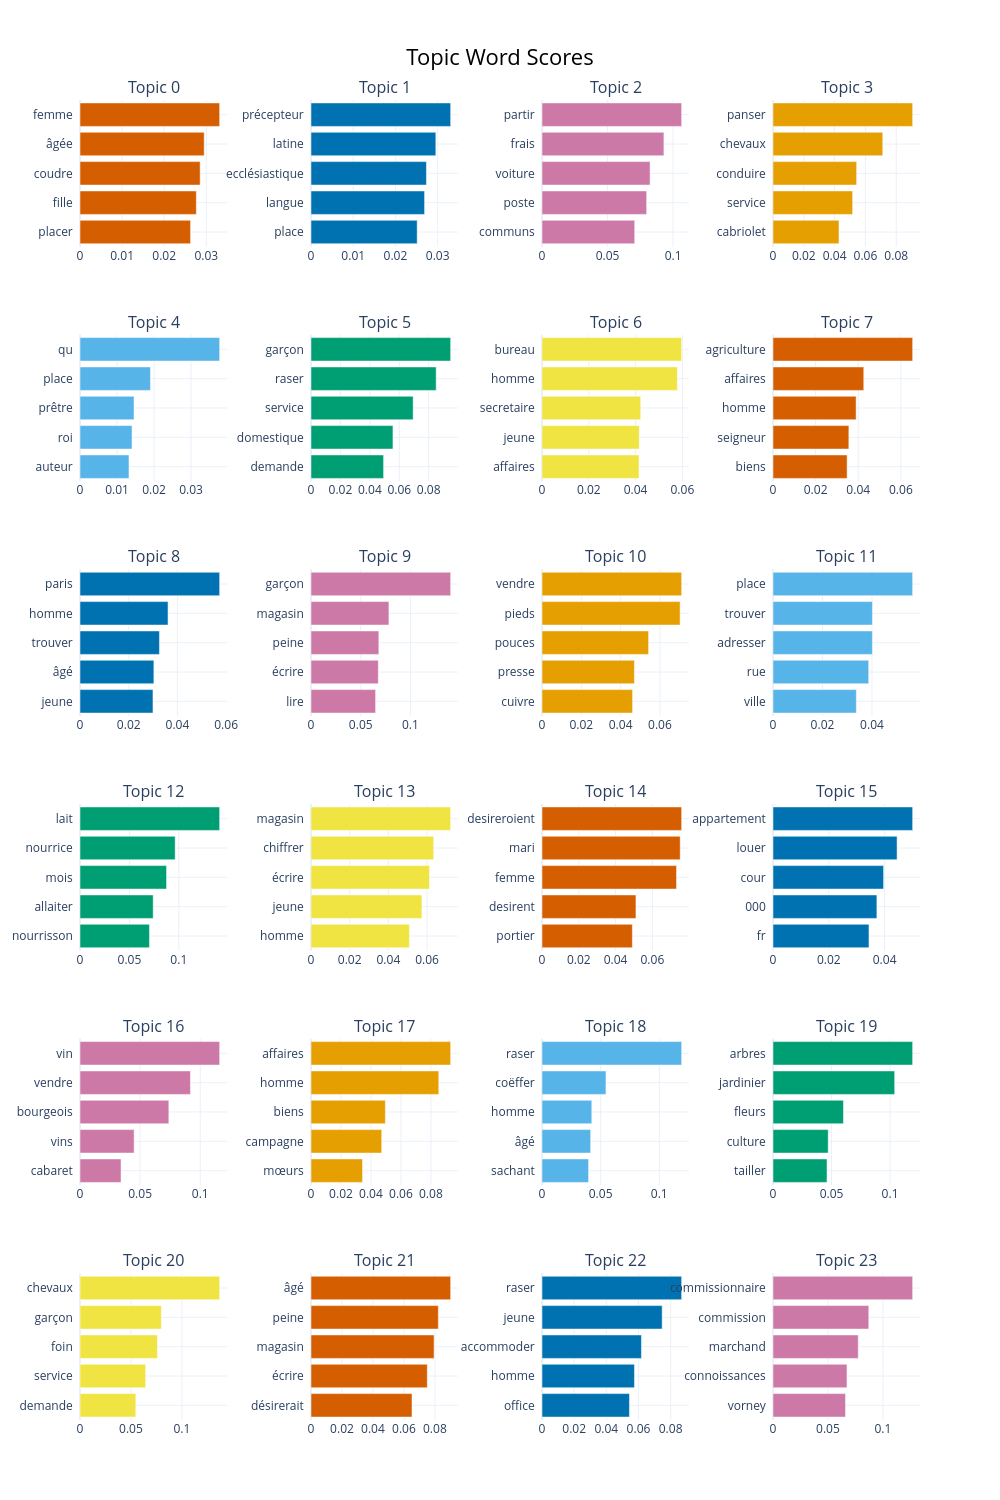
\includegraphics[width=15cm]{plot_bertopic.png}
	\caption{Vingt-quatre \textit{topics} générés par BERTopic}
\end{figure}

\begin{figure}[h!t]
	\centering
	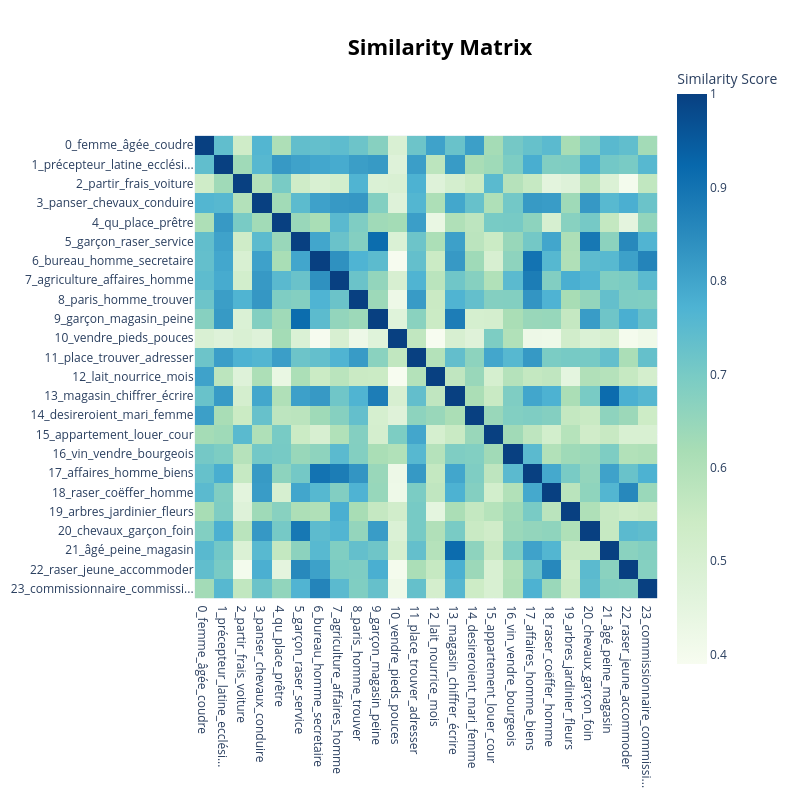
\includegraphics[width=12cm]{matrice_bertopic.png}
	\caption{Matrice de similarité entre les \textit{topics} générés par BERTopic}
\end{figure}



Deux \textit{topics}, cependant, révélateurs de segments très particuliers du marché du travail, n'apparaissent qu'avec BERTopic. Il s'agit tout d'abord du \textit{topic} 12, dédié aux nourrices en recherche d'emploi, que je n'ai pas pu traiter dans le cadre de ce travail en raison de leur très faible présence dans les \textit{Affiches} (moins de 50 occurrences). Néanmoins, il ne parait pas étonnant que le modèle parvienne à différencier les annonces de nourrices du reste des annonces d'emploi, tant le vocabulaire et les formules qui y sont employées diffèrent du reste du corpus: ici, pas (ou peu) de mention de compétences manuelles ou de connaissances de certaines langues, les informations données ont principalement trait à la santé de la nourrice, à la qualité et à l'âge de son lait. Par exemple, cette annonce lyonnaise en date du 15 décembre 1803, où "une jeune Veuve qui jouit de la meilleure santé, et dont le lait a vingt mois, [désire] trouver un Nourrisson pour l'allaiter chez elle\footnote{\textit{Affiches de Lyon}, 15 décembre 1803}", est très représentative.

Le second \textit{topic} unique à BERTopic est le \textit{topic} 19, consacré aux annonces de jardiniers. Rattaché à la domesticité spécialisée et de plus en plus demandée au XVIIIè siècle avec l'avènement des jardins urbains\footcites{synowieckiParisSesJardins2021}, le jardinier se distingue des autres domestiques qualifiés en ce qu'il n'exerce pas une activité à proprement dit intellectuelle. Cette différence se ressent dans les mots employés dans les annonces, qui relèvent de compétences artistiques mais surtout physiques (tailler) et doivent également signifier les connaissances précises et quasi-scientifiques acquises par le domestique dans son domaine (connaissance des différentes cultures, des soins des fleurs comme des arbres). Sa présence comme \textit{topic} distinct n'est donc pas étonnante tant sa recherche d'emploi se distingue de celle des autres serviteurs, par son exercice à l'extérieur du foyer autant que par son caractère pluriel, à la fois manuel et très spécialisé. 




\section{Resituer les \textit{topics} géographiquement et chronologiquement}

\subsection{Le \textit{topic modeling} par ville}

Enfin, j'ai décidé de conclure cette incursion dans les annonces en tirant parti de deux fonctionnalités fournies par BERTopic: le \textit{topic modeling} par classe et le \textit{topic modeling} roulant, ou dynamique. Pour ces deux analyses, j'ai dû, face aux déséquilibres du corpus initial (surreprésentation de Lyon et du début du XIXè siècle notamment), créer des jeux de données spécifiques. Les \textit{topics} présentés ne seront donc pas les mêmes que ceux de la partie précédente, et le mode de constitution des nouveaux corpus (par sélection aléatoire, avec doublons dans le cas où les annonces manqueraient, comme pour Bordeaux) appelle à la prudence. 

\begin{figure}[h!t]
	\centering
	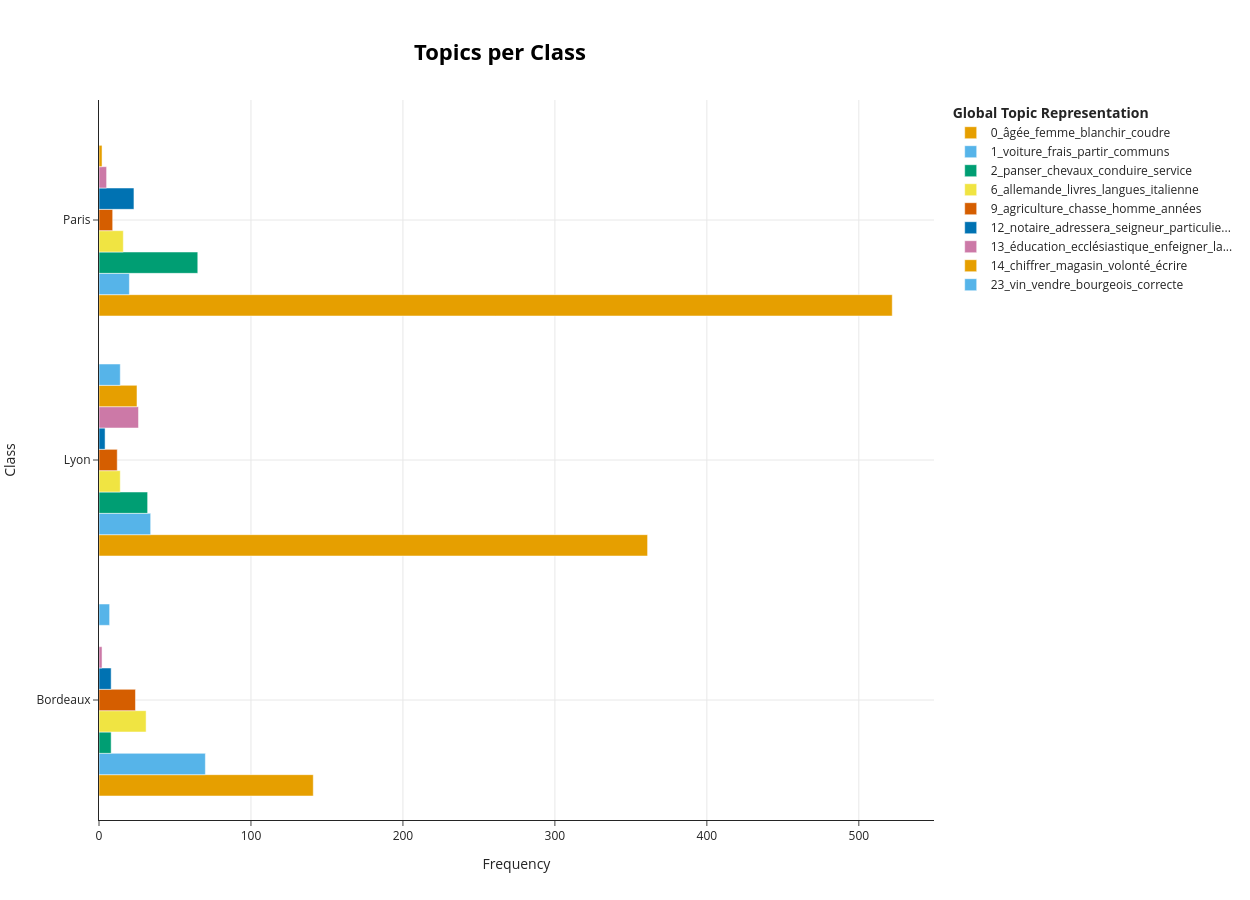
\includegraphics[width=15cm]{bertopic_villes.png}
	\caption{Résultat du \textit{topic modeling} par ville avec BERTopic}
\end{figure}

Les graphique obtenu permet ainsi de mesurer le poids de chaque ville dans la génération des topics: si Paris est surreprésenté parmi les annonces d'emplois domestiques manuels (\textit{topics} 0 "femme, blanchir, coudre" et 2 "panser, chevaux, conduire"), Bordeaux et Lyon semblent plus concernées par la domesticité qualifiée (\textit{topics} 6, 13 et 14) ainsi que le commerce de vin (\textit{topic} 23).

\subsection{Le\textit{ topic modeling} roulant dans le temps}

Quant à lui, le \textit{topic modeling }roulant, s'il s'annonçait prometteur pour capter les évolutions du marché de l'emploi domestique sur la période étudiée, semble malheureusement trop dépendant des lacunes du corpus, et ce malgré le rééquilibrage effectué. L'intervalle 1783-1795, pour lequel aucun numéro n'est disponible, rend difficile l'interprétation des données restantes. Tous les \textit{topics} ou presque semblent connaître des variations entre 1750 et 1805, mais celles-ci semblent plus liées aux variations internes au corpus.


\begin{figure}[h!t]
	\centering
	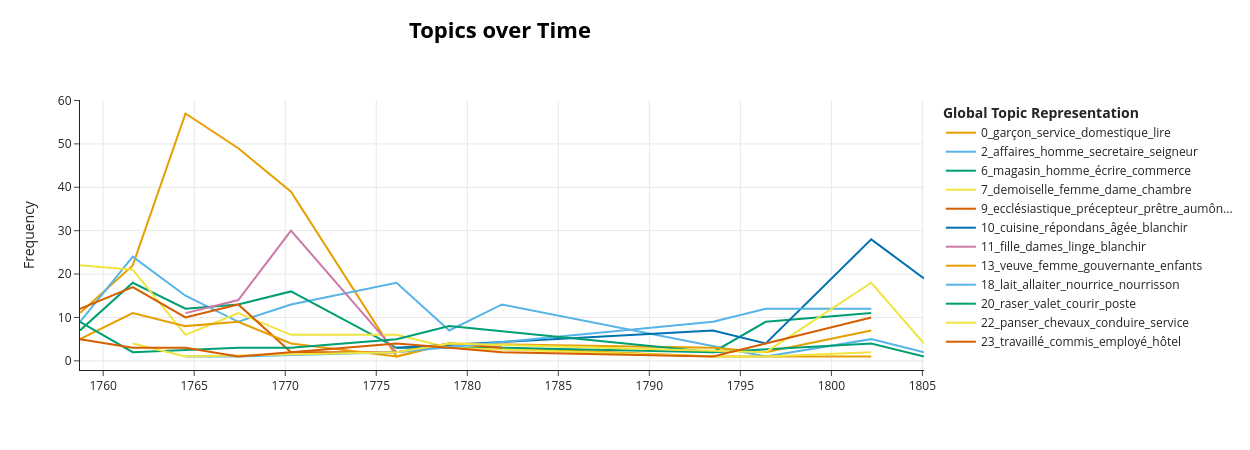
\includegraphics[width=15cm]{bertopic_temps.png}
	\caption{Résultat du \textit{topic modeling} dynamique avec BERTopic}
\end{figure}
	\part*{Conclusion}
\addcontentsline{toc}{part}{Conclusion}
\markboth{Conclusion}{Conclusion}


Un des résultats méthodologiques forts de ce mémoire a d'abord été de montrer qu'un traitement automatisé des journaux de petites annonces est possible, notamment grâce à l'entraînement de modèles d'apprentissage pour l'extraction et la catégorisation d'entités, mais également en tirant profit de l'uniformité formelle des annonces pour employer des expressions régulières. 

Les incursions vers les différentes composantes des demandes d'emploi ont permis de montrer en quoi l'annonce n'est pas un support qui vient perturber de bout en bout la recherche de travail à l'époque moderne. Au contraire, elle perpétue par beaucoup d'aspects les processus et les structures du marché de l'emploi domestique aux XVIIIè-XIXè siècles: le marché des annonces reste majoritairement mixte, occupé par des domestiques peu qualifiés, jeunes et aux savoir-faire manuels. L'emploi reste conditionné à l'intervention de multiples intermédiaires et garants dans le processus de recrutement, dont l'annonce n'est finalement qu'une composante parmi d'autres. 

Mais, ponctuellement, ou selon certaines modalités bien précises, l'annonce peut s'éloigner de la norme domestique, et refléter les transformations qui accompagnent l'évolution de la condition et de la conjecture économique à la fin de l'Ancien Régime. Ainsi, j'ai pu montrer dans la troisième partie, en continuité avec les travaux d'Ulrike Krampl, que la domesticité des annonces n'est pas le reflet exact de la domesticité dans son ensemble, mais plutôt son miroir déformé: y sont surreprésentés des hommes domestiques qualifiés, professeurs, secrétaires ou régisseurs, pour qui le format des annonces s'inscrit en continuité directe de leur pratique quotidienne de l'écriture. Le lectorat des annonces, plutôt bourgeois, représente également une cible intéressante pour ces domestiques spécialisés, qui n'officient généralement quand dans les grandes maisons. 

L'étude du genre dans les annonces a également permis de mettre en évidence la reconduction sur le papier de certains processus déjà connus de la discipline historique: le cantonnement des femmes à certaines tâches domestiques, le contrôle social qui s'impose à elles et les obligent à mettre en avant leur probité devant d'éventuelles employeurs. 

Enfin, l'étude numérique des petites annonces a permis d'interroger les raisons de l'usage de ce support par les domestiques. Face à la subsistance des réseaux informels, pourquoi se donner la peine d'aller jusqu'au Bureau d'adresses, de (parfois) payer une annonce, puis se soumettre au hasard et aux potentiels risques de l'emploi par un maître inconnu? Si l'historiographie a pu soulever les hypothèses très probables de la saturation du marché traditionnel du travail\footcites{pasleauAnnoncesEmploiLiege2002}{sarasuaCriadosNodrizasAmos1994} ou de la crise économique qui joue en faveur des maîtres et invite à multiplier les méthodes de recherche, je pense qu'il est également important d'envisager les avantages et les espaces de liberté que peuvent procurer les annonces, tout particulièrement à l'aune des difficultés structurelles que je viens de mentionner. Certaines déclarations des domestiques, notamment relatives aux bureaux de placement, doivent permettre de penser l'annonce comme espace émancipatoire, bien que hautement contraint, qui permet d'échapper en partie aux constrictions du placement. Pour les domestiques qui viennent d'arriver en ville, n'ont ni réseau ni voisins, ou qui souhaitent changer d'emploi sans le faire savoir à leur entourage, on peut également imaginer que l'annonce représente une possibilité bienvenue.
 
Cette étude du marché de la domesticité au moyen des méthodes numériques a ainsi permis d'obtenir plusieurs résultats intéressants aussi bien pour l'histoire du genre que du travail ou de la presse. Si certaines problématiques (les questions des offres d'emploi, des domestiques étrangers, des voyages ou de la mobilité des annonces et des informations en dehors de la ville, pour ne citer qu'elles) ont été laissées de côté, ou traitées moins exhaustivement, j'espère malgré tout avoir pu montrer l'intérêt des méthodes numériques pour faire une histoire, non pas forcément massive, mais riche et socialement située de groupes et d'individus souvent écartés du récit historique. 




 
	
	
	% annexes
	\part*{Annexes}
\addcontentsline{toc}{part}{Annexes}
\markboth{Annexes}{Annexes}


\section{Accès aux données du mémoire}

Code, notebooks, données et version \LaTeX du mémoire disponibles sur Github : \url{https://github.com/mailanlopez/domestiques_annonces}.


\newpage
\section{Constitution détaillée du corpus}

\begin{table}[ht]
	\centering
	\caption{Noms, identifiants et nombre des numéros des \textit{Affiches} de Paris intégrés au corpus}
	\resizebox{\textwidth}{!}{%
		\begin{tabular}{lcccc}
			\hline
			\multicolumn{1}{c}{\textbf{Titre}}                                     & \multicolumn{1}{c}{\textbf{Identifiant ark}} & \multicolumn{1}{c}{\textbf{Année}} & \multicolumn{1}{c}{\textbf{No. dispo.}} & \multicolumn{1}{c}{\textbf{No. récup.}} \\ \hline
			\textit{Annonces, affiches et avis divers}                               & 12148/cb42141882c                             & 1752                                & 35                                                & 35                                              \\ 
			\textit{Annonces, affiches et avis divers}                               & 12148/cb42141882c                             & 1753                                & 52                                                & 52                                              \\ 
			\textit{Annonces, affiches et avis divers}                               & 12148/cb42141882c                             & 1754                                & 52                                                & 52                                              \\ 
			\textit{Annonces, affiches et avis divers}                               & 12148/cb32695181v                             & 1756                                & 99                                                & 52                                              \\ 
			\textit{Annonces, affiches et avis divers}                               & 12148/cb32695181v                             & 1757                                & 100                                               & 51                                              \\ 
			\textit{Annonces, affiches et avis divers}                               & 12148/cb32695181v                             & 1758                                & 98                                                & 50                                              \\ 
			\textit{Annonces, affiches et avis divers}                               & 12148/cb32695181v                             & 1759                                & 101                                               & 51                                              \\ 
			\textit{Annonces, affiches et avis divers}                               & 12148/cb32695181v                             & 1760                                & 100                                               & 51                                              \\ 
			\textit{Annonces, affiches et avis divers}                               & 12148/cb32695181v                             & 1761                                & 101                                               & 53                                              \\ 
			\textit{Annonces, affiches et avis divers}                               & 12148/cb32695181v                             & 1762                                & 100                                               & 52                                              \\ 
			\textit{Annonces, affiches et avis divers}                               & 12148/cb32695181v                             & 1763                                & 101                                               & 50                                              \\ 
			\textit{Annonces, affiches et avis divers}                               & 12148/cb32695181v                             & 1764                                & 101                                               & 50                                              \\ 
			\textit{Annonces, affiches et avis divers}                               & 12148/cb32695181v                             & 1765                                & 100                                               & 50                                              \\ 
			\textit{Annonces, affiches et avis divers}                               & 12148/cb32695181v                             & 1766                                & 100                                               & 50                                              \\ 
			\textit{Annonces, affiches et avis divers}                               & 12148/cb32695181v                             & 1768                                & 100                                               & 49                                              \\ 
			\textit{Annonces, affiches et avis divers}                               & 12148/cb32695181v                             & 1769                                & 100                                               & 48                                              \\ 
			\textit{Annonces, affiches et avis divers}                               & 12148/cb32695181v                             & 1771                                & 100                                               & 49                                              \\ 
			\textit{Annonces, affiches et avis divers}                               & 12148/cb32695181v                             & 1772                                & 101                                               & 50                                              \\ 
			\textit{Annonces, affiches et avis divers}                               & 12148/cb32695181v                             & 1773                                & 99                                                & 50                                              \\ 
			\textit{Annonces, affiches et avis divers}                               & 12148/cb32695181v                             & 1774                                & 100                                               & 49                                              \\ 
			\textit{Annonces, affiches et avis divers}                               & 12148/cb32695181v                             & 1775                                & 100                                               & 49                                              \\ 
			\textit{Annonces, affiches et avis divers}                               & 12148/cb32695181v                             & 1776                                & 101                                               & 52                                              \\ 
			\textit{Affiches, annonces et avis divers}                               & 12148/cb32683020p                             & 1777                                & 53                                                & 53                                              \\ 
			\textit{Affiches, annonces et avis divers}                               & 12148/cb32683020p                             & 1778                                & 52                                                & 49                                              \\ 
			\textit{Affiches, annonces et avis divers}                               & 12148/cb32683020p                             & 1779                                & 52                                                & 52                                              \\ 
			\textit{Affiches, annonces et avis divers}                               & 12148/cb32683020p                             & 1780                                & 52                                                & 52                                              \\ 
			\textit{Annonces, affiches et avis divers}                               & 12148/cb32695181v                             & 1781                                & 2                                                 & 0                                               \\ 
			\textit{Annonces, affiches et avis divers}                               & 12148/cb32695181v                             & 1782                                & 2                                                 & 0                                               \\ 
			\textit{Affiches, annonces et avis divers, ou Journal général de France} & 12148/cb32683112b                             & 1789                                & 2                                                 & 0                                               \\ 
			\textit{Affiches, annonces et avis divers, ou Journal général de France} & 12148/cb32683112b                             & 1790                                & 1                                                 & 0                                               \\ 
			\textit{Affiches, annonces et avis divers, ou Journal général de France} & 12148/cb32683112b                             & 1793                                & 10                                                & 0                                               \\ 
			\textit{Affiches, annonces et avis divers, ou Journal général de France} & 12148/cb32683112b                             & 1794                                & 5                                                 & 0                                               \\ 
			\textit{Affiches, annonces et avis divers, ou Journal général de France} & 12148/cb32683112b                             & 1804                                & 87                                                & 72                                              \\ 
			\textit{Affiches, annonces et avis divers, ou Journal général de France} & 12148/cb32683112b                             & 1807                                & 93                                                & 92                                              \\ 
			\textit{Affiches, annonces et avis divers, ou Journal général de France} & 12148/cb32683112b                             & 1808                                & 32                                                & 0                                               \\ 
			\textit{Affiches, annonces et avis divers, ou Journal général de France} & 12148/cb32683112b                             & 1814                                & 62                                                & 0                                               \\ \hline
	\end{tabular}}
\end{table}



\begin{table}[h]
	\centering
	\caption{Noms, identifiants et nombre des numéros des \textit{Affiches} de Lyon intégrés au corpus}
	\resizebox{\textwidth}{!}{%
		\begin{tabular}{lcccc}
			\hline
			\multicolumn{1}{c}{\textbf{Titre}}               & \multicolumn{1}{c}{\textbf{Identifiant ark}} & \multicolumn{1}{c}{\textbf{Année(s)}} & \multicolumn{1}{c}{\textbf{No. dispo.}} & \multicolumn{1}{c}{\textbf{No. récup.}} \\ \hline
			\textit{Les Affiches de Lyon, avis divers, etc.}   & 75584/pf0002006730                            & 1750                                   & 52                                                & 52                                              \\ 
			\textit{Affiches de Lyon, annonces et avis divers} & 75584/pf0002006730                            & 1759-1760                              & 105                                               & 105                                             \\ 
			\textit{Affiches de Lyon, annonces et avis divers} & 75584/pf0002006730                            & 1761-1762                              & 105                                               & 105                                             \\ 
			\textit{Affiches de Lyon, annonces et avis divers} & 75584/pf0002006730                            & 1763-1764                              & 104                                               & 104                                             \\ 
			\textit{Affiches de Lyon, annonces et avis divers} & 75584/pf0002006730                            & 1765-1766                              & 107                                               & 107                                             \\ 
			\textit{Affiches de Lyon, annonces et avis divers} & 75584/pf0002006730                            & 1767-1768                              & 106                                               & 106                                             \\ 
			\textit{Affiches de Lyon, annonces et avis divers} & 75584/pf0002006730                            & 1769-1770                              & 111                                               & 111                                             \\ 
			\textit{Affiches de Lyon, annonces et avis divers} & 75584/pf0002006730                            & 1771-1772                              & 109                                               & 109                                             \\ 
			\textit{Affiches, annonces et avis divers de Lyon} & 75584/pf0002006730                            & Ans 	3-4-5 (1795-1796-1797)            & 184                                               & 184                                             \\ 
			\textit{Petites affiches de Lyon}                  & 75584/pf0002006730                            & Ans 6-7 (1802-1803-1804)               & 208                                               & 208                                             \\ \hline
	\end{tabular}}
\end{table}


\begin{table}[ht]
	\centering
	\caption{Noms, identifiants et nombre des numéros des \textit{Affiches} de Bordeaux intégrés au corpus}
	\resizebox{\textwidth}{!}{%
		\begin{tabular}{lcccc}
			\hline
			\multicolumn{1}{c}{\textbf{Titre}}                                 & \multicolumn{1}{c}{\textbf{Cote}} & \multicolumn{1}{c}{\textbf{Année}} & \multicolumn{1}{c|}{\textbf{No. dispo.}} & \multicolumn{1}{c}{\textbf{No. récup.}} \\ \hline
			\textit{Annonces, affiches et avis divers pour la ville de Bordeaux} & PN\_0003                           & 1758                                & 22                                                & 5                                               \\ 
			\textit{Annonces, affiches et avis divers pour la ville de Bordeaux} & PN\_0003                           & 1759                                & 52                                                & 12                                              \\ 
			\textit{Annonces, affiches et avis divers pour la ville de Bordeaux} & PN\_0003                           & 1760                                & 52                                                & 12                                              \\ 
			\textit{Annonces, affiches et avis divers pour la ville de Bordeaux} & PN\_0003                           & 1761                                & 53                                                & 12                                              \\ 
			\textit{Annonces, affiches et avis divers pour la ville de Bordeaux} & PN\_0003                           & 1762                                & 52                                                & 12                                              \\ 
			\textit{Annonces, affiches et avis divers pour la ville de Bordeaux} & PN\_0003                           & 1763                                & 52                                                & 12                                              \\ 
			\textit{Annonces, affiches et avis divers pour la ville de Bordeaux} & PN\_0003                           & 1764                                & 52                                                & 12                                              \\ 
			\textit{Annonces, affiches et avis divers pour la ville de Bordeaux} & PN\_0003                           & 1765                                & 52                                                & 12                                              \\ 
			\textit{Annonces, affiches et avis divers pour la ville de Bordeaux} & PN\_0003                           & 1766                                & 52                                                & 12                                              \\ 
			\textit{Annonces, affiches et avis divers pour la ville de Bordeaux} & PN\_0003                           & 1767                                & 53                                                & 12                                              \\ 
			\textit{Annonces, affiches et avis divers pour la ville de Bordeaux} & PN\_0003                           & 1768                                & 52                                                & 12                                              \\ 
			\textit{Annonces, affiches et avis divers pour la ville de Bordeaux} & PN\_0003                           & 1769                                & 52                                                & 12                                              \\ 
			\textit{Annonces, affiches et avis divers pour la ville de Bordeaux} & PN\_0003                           & 1771                                & 44                                                & 12                                              \\ 
			\textit{Annonces, affiches et avis divers pour la ville de Bordeaux} & PN\_0003                           & 1772                                & 45                                                & 12                                              \\ 
			\textit{Annonces, affiches et avis divers pour la ville de Bordeaux} & PN\_0003                           & 1773                                & 1                                                 & 0                                               \\ 
			\textit{Annonces, affiches et avis divers pour la ville de Bordeaux} & PN\_0003                           & 1777                                & 49                                                & 12                                              \\ 
			\textit{Annonces, affiches et avis divers pour la ville de Bordeaux} & PN\_0003                           & 1778                                & 53                                                & 12                                              \\ 
			\textit{Annonces, affiches et avis divers pour la ville de Bordeaux} & PN\_0003                           & 1779                                & 52                                                & 12                                              \\ 
			\textit{Annonces, affiches et avis divers pour la ville de Bordeaux} & PN\_0003                           & 1780                                & 52                                                & 12                                              \\ 
			\textit{Annonces, affiches et avis divers pour la ville de Bordeaux} & PN\_0003                           & 1781                                & 52                                                & 12                                              \\ 
			\textit{Annonces, affiches et avis divers pour la ville de Bordeaux} & PN\_0003                           & 1782                                & 43                                                & 12                                              \\ 
			\textit{Annonces, affiches et avis divers pour la ville de Bordeaux} & PN\_0003                           & 1783                                & 80                                                & 11                                              \\ 
			\textit{Annonces, affiches et avis divers pour la ville de Bordeaux} & PN\_0003                           & 1784                                & 1                                                 & 0                                               \\ \hline
	\end{tabular}}
\end{table}




	\backmatter
	
	\addcontentsline{toc}{chapter}{Bibliographie}
	
	\nocite{agrenMakingHerTurn2018, lindstromMistressMaidStructure2017, feyelAuxOriginesRubrique2012, kalifaCivilisationJournalHistoire2011,feyelPressePubliciteFrance2003, rocheVillePromiseMobilite2000, fargeDireMalDire201, mekaoui-cheboutOppressionsEmbaucheChercher2020, manskerAmourFictionVoyeurisme2020, frydmanDessousPetitesAnnonces2020, cuvelierAfficheAvantAffiche2020, cuvelierVilleCaptiveeAffichage2019, manskerMarriagesPetitesAffiches2018,tantnerAncetresMoteursRecherche2017,jungApparieurMarchandTravail2017,caracausiIntroductionPourHistoire2017,casaliniRetourFeminisationProfessionnalisation2009,margairazInformationEconomiqueXVIeXIXe2008, pasleauProceedingsServantProject2001,fauve-chamouxServantsPreindustrialEurope1998,fauve-chamouxSurplusUrbainFemmes1998a,chamouxPhenomeneDomesticiteEurope1997,zellerRapportsAncillairesMobilite1992,fairchildsDomesticEnemiesServants1984,mcbrideSocialMobilityLower1974,petitfrereOeilMaitreMaitres1986a,godineauTravailPolitiqueParis1986,angelovTop2VecDistributedRepresentations2020,petterssonSpellingNormalisationLinguistic2016,agrenPeeringDarknessUses2014,petterssonVerbPhraseExtraction2014,bealChampsAuxCuisines2019,sartiHistoriansSocialScientists2014,rochePeupleParisEssai1981}
	\printbibliography
	
	% glossaire
	%\include{back/glossaire}
	
	% Liste des figures
	\listoffigures
	% table des tableaux
	\listoftables
	
	
\end{document}